% This is the Reed College LaTeX thesis template. Most of the work
% for the document class was done by Sam Noble (SN), as well as this
% template. Later comments etc. by Ben Salzberg (BTS). Additional
% restructuring and APA support by Jess Youngberg (JY).
% Your comments and suggestions are more than welcome; please email
% them to cus@reed.edu
%
% See http://web.reed.edu/cis/help/latex.html for help. There are a
% great bunch of help pages there, with notes on
% getting started, bibtex, etc. Go there and read it if you're not
% already familiar with LaTeX.
%
% Any line that starts with a percent symbol is a comment.
% They won't show up in the document, and are useful for notes
% to yourself and explaining commands.
% Commenting also removes a line from the document;
% very handy for troubleshooting problems. -BTS

% As far as I know, this follows the requirements laid out in
% the 2002-2003 Senior Handbook. Ask a librarian to check the
% document before binding. -SN

%%
%% Preamble
%%
% \documentclass{<something>} must begin each LaTeX document
\documentclass[11pt,twoside]{reedthesis}
\usepackage[paperheight=237mm,paperwidth=168mm,bottom=20mm, top=20mm, outer=1.5cm, inner=2.4cm]{geometry}
% Packages are extensions to the basic LaTeX functions. Whatever you
% want to typeset, there is probably a package out there for it.
% Chemistry (chemtex), screenplays, you name it.
% Check out CTAN to see: http://www.ctan.org/
%%
\usepackage{graphicx,latexsym}
\usepackage{amsmath}
\usepackage{amssymb,amsthm}
\usepackage{longtable,booktabs,setspace}
\usepackage{chemarr} %% Useful for one reaction arrow, useless if you're not a chem major
\usepackage[hyphens]{url}
% Added by CII
\usepackage{hyperref}
\usepackage{lmodern}
\usepackage{float}
\floatplacement{figure}{H}
% End of CII addition
\usepackage{rotating}

% Next line commented out by CII
%%% \usepackage{natbib}
% Comment out the natbib line above and uncomment the following two lines to use the new
% biblatex-chicago style, for Chicago A. Also make some changes at the end where the
% bibliography is included.
%\usepackage{biblatex-chicago}
%\bibliography{thesis}


% Added by CII (Thanks, Hadley!)
% Use ref for internal links
\renewcommand{\hyperref}[2][???]{\autoref{#1}}
\def\chapterautorefname{Chapter}
\def\sectionautorefname{Section}
\def\subsectionautorefname{Subsection}
% End of CII addition

% Added by CII
\usepackage{caption}
\captionsetup{width=5in}
% End of CII addition

% \usepackage{times} % other fonts are available like times, bookman, charter, palatino

% Syntax highlighting #22

% To pass between YAML and LaTeX the dollar signs are added by CII
\title{Global ecological drivers of transpiration regulation in woody plants}
\author{Víctor Flo Sierra}
% The month and year that you submit your FINAL draft TO THE LIBRARY (May or December)
\date{Dec 2020}
\degree{DOCTORADO EN ECOLOGIA TERRESTRE}
% \division{}
\advisor{Rafael Poyatos López}
\institution{Autonomous University of Barcelona}
% \degree{DOCTORADO EN ECOLOGIA TERRESTRE}
%If you have two advisors for some reason, you can use the following
% Uncommented out by CII
\altadvisor{Jordi Martínez Vilalta}
% End of CII addition

%%% Remember to use the correct department!
\department{Centre de Recerca Ecològica i Aplicacions Forestals}
% if you're writing a thesis in an interdisciplinary major,
% uncomment the line below and change the text as appropriate.
% check the Senior Handbook if unsure.
%\thedivisionof{The Established Interdisciplinary Committee for}
% if you want the approval page to say "Approved for the Committee",
% uncomment the next line
%\approvedforthe{Committee}

% Added by CII
%%% Copied from knitr
%% maxwidth is the original width if it's less than linewidth
%% otherwise use linewidth (to make sure the graphics do not exceed the margin)
\makeatletter
\def\maxwidth{ %
  \ifdim\Gin@nat@width>\linewidth
    \linewidth
  \else
    \Gin@nat@width
  \fi
}
\makeatother

\renewcommand{\contentsname}{Table of Contents}
% End of CII addition

\setlength{\parskip}{0pt}

% Added by CII

\providecommand{\tightlist}{%
  \setlength{\itemsep}{0pt}\setlength{\parskip}{0pt}}

\Acknowledgements{
\setlength{\parindent}{30pt} A pesar de ser firme defensora de que la
tesis no supone un mérito excepcional digno de especiales
reconocimientos, no desperdiciaré la oportunidad de agradecer todo lo
vivido durante estos años y dejar grabado lo mucho que deben estas
páginas a las personas que me rodean.\par
Durante esta etapa, que empezó cuando llegué a Barcelona, he tenido la
suerte de encontrar a personas maravillosas, de viajar por el mundo y de
aprender sobre diferentes aspectos de la vida. Quiero agradecer en
primer lugar, a la que fue mi primera familia en Catalunya, mis
compañeros de máster, en especial a Estrella, Aida, Alba, Aina, Carla,
Enrique, John y Gustavo y a mis compañeros de piso Laura y Josan.
Gracias por los ratos en el césped, las visitas a Mataró y las noches
arreglando el mundo en el \emph{Cop de ma}, gracias, en definitiva, por
hacerme sentir en casa.\par
Cuando una empieza la tesis le dicen que debería preocuparse de escoger
bien a sus directores porque son personas con las que tendrá que
compartir cuatro años y ver más a menudo que a sus propios padres. Yo
con Paco apenas tuve dos reuniones antes de solicitar el doctorado.
Después de estos más de cuatro años trabajando juntos sé que si volviese
atrás volvería a elegirte. Gracias Paco por el ejemplo, por las charlas
en los viajes, por tu forma de pensar tan crítica, transversal y
profunda, por enseñarme tanto más allá de lo estrictamente
académico\ldots{} A Miguel Ángel lo conocía más. Fui su alumna durante
la carrera y sé que pocas personas tienen un conocimiento más holístico
de la naturaleza murciana, mayor integridad y devoción por su trabajo.
Gracias por tu visión naturalista y aplicada, gracias por las charlas de
política y las explicaciones sobre el Mar Menor. Durante estos años he
crecido con y gracias a vosotros, y no podría sentirme más
afortunada.\par
Además esta tesis no hubiese tenido los mismos resultados sino hubiese
compartido las dudas, preocupaciones, alegrías y el desánimo con tantos
buenos compañeros. Gracias a los compañeros de despacho, a Anna, Javi,
Judit, Carlos, Manu, Marta, Pere y Pol. Sin duda las penas han sido
menos penas con vosotros y las fiestas, almuerzos y barbacoas mucho más
divertidas. Gracias por las risas y la terapia de grupo. No me
acostumbro a pensar en un trabajo sin vosotros.\par
Gracias también a los compañeros de grupo. Enric, Jordi, Luciana y
Nuria, el \emph{phoskitos lab} no podría tener mejor plantilla. Con
vosotros se demuestra que hacer ciencia no está reñido con un ambiente
laboral de calidad, colaborativo, respetuoso y divertido. Gracias por
tantos buenos momentos, por las discusiones académicas y las no tan
académicas, por las salidas a la montaña y las jornadas de convivencia
en los congresos. Quiero agradecer también a mis compañeros de
departamento en Murcia. Gracias a Paqui, Juan Miguel y Pablo por el
trabajo de campo y de despacho, por estar siempre ahí pese a la
distancia, por no haber dudado en ayudar siempre que lo he necesitado.
Gracias también a Guillem por las semanas de trabajo y convivencia en
Murcia y tus dosis de amabilidad y optimismo, a Pep Serra y Gerard Sapes
por los sabios consejos y la inspiración.\par
Durante estos últimos años también he tenido la oportunidad de librarme
de los calurosos veranos catalanes y murcianos escapándome de estancia a
otros países. Gracias a Jens-Christian por la acogida en Aarhus y a
Antoine y Olivier por la estancia en Suiza. Me quedo con el recuerdo de
los paseos en bici por Dinamarca y la estampa de los Alpes por la
ventana del despacho y las barbacoas en el lago Leman. Gracias también a
los que han estado siempre ahí, a los amigos de toda la vida, Jose,
Maria José, Mari Nieves, Maria Victoria, Álvaro Talavera y Pedro.
Gracias por estar tan cerca a pesar de los kilómetros, gracias por las
visitas, por aguantar con paciencia mis quejas sobre política y ciencia,
por los cafés, las terapias y el consuelo. Gracias también a Victor
Valero por el tiempo que hemos pasado juntos en Barcelona, por las horas
de desahogo mutuo y los planes culturales.\par
Quiero agradecer también a mi familia. A mis tios, por ayudarme siempre
que les ha sido posible. A mi hermano mayor, por plantar en mi la
semilla del amor por la naturaleza, sin tu ejemplo no hubiese dado los
primeros pasos del camino que ahora completo. Gracias también a mi
hermano mellizo por la ayuda incondicional e implicación, llegando
incluso a armarte con botas y cinta métrica para echar una mano en el
trabajo de campo.\par
Gracias sobre todo a quien desde hace más de tres años es mucho más que
un compañero de despacho. Gracias Víctor por tu compresión, tu
paciencia, tus consejos y buenas ideas. Estas páginas te deben mucho.
Gracias por animarme y hacerme ver siempre el vaso medio lleno. Por
darme una segunda familia en Catalunya.\par
Gracias finalmente a mis padres, a quienes una época cruel y la falta de
recursos les despojó de la oportunidad para completar etapas académicas
más allá de los estudios más elementales. Sabed que no habría sido
posible llegar hasta aquí sin vosotros.\par
}

\Dedication{
\vspace*{4.5cm}
\begin{flushright}
\hfil \textit{Lo que nos diferencia de otros seres vivos} \break
\hfil \textit{no es la capacidad de perturbar el planeta,} \break
\hfil \textit{sino la voluntad de salvarlo.}
\end{flushright}
\vspace*{\fill}
}

\Preface{

}

\Abstract{
\setlength{\parindent}{30pt} Understanding how climate affects species'
distribution and performance is a central issue in ecology since its
origins. In last decades, however, the interest in this question has
been reactivated by the current context of climate change. Species Niche
Modelling has been widely used to assess shifts in species distribution
and to test the relationship between species' climatic niche and species
physiological and demographic performance, implicitly assuming that
species occurrence portrays the environmental and biotic species'
suitable conditions. Nevertheless it is still largely undetermined
whether these models can portray population and community responses,
particularly in relation to extreme climatic episodes.\par

In this thesis I aim at exploring the capacity of niche modelling to
predict species decay under extreme climatic conditions, particularly
droughts, addressing some constraints of this approach and proposing
possible solutions. To achieve this goal, I counted with 3 vegetation
decay datasets measured in the Spanish SE after the extreme drought year
2013-2014. Two of these datasets were based on defoliation sampling of
individual plants belonging to more than 40 semiarid shrubland species
(chapters 2, 4 and 5), while the other one was based on regional
compiled data of \emph{Pinus halepensis} L. affectation in plots of
\(1 km^2\) (chapter 3). In second chapter I used different Species
Distribution Model (SDMs) algorithms to estimate species' climatic
suitability before (1950-2000) and during the extreme drought, in order
to test the possible correlation between suitability and decay, and
whether the existence of this relationship depended on the applied SDM
algorithm. I consistently found a positive correlation between remaining
green canopy and species' climatic suitability before the event,
suggesting that populations historically living closer to their species'
tolerance limits are more vulnerable to drought. Contrastingly,
decreased climatic suitability during the drought period did not
correlate with remaining green canopy, likely because of extremely low
climatic suitability values achieved during the exceptional climatic
episode. In order to test whether this extremely low suitability values
could derive as a consequence of only considering climatic averages when
calibrating SDMs, in the third chapter I developed a method to include
inter-annual climatic variability into niche characterization. I then
compared the respective capacities of climatic suitabilities obtained
from averaged-based and from inter-annual variability-based niches to
explain demographic responses to extreme climatic events. I found that
climatic suitability obtained from both niches quantifications
significantly explained species demographic responses. However, climatic
suitability from inter-annual variability-based niches showed higher
explanatory capacity, especially for populations that tend to be more
geographically marginal. In the fourth chapter I tried to overcome the
inability of the SDMs to predict populations decay during extreme
conditions, as observed in the second chapter, by using Euclidean
distances to species' niche in the environmental space. I compared the
capacities of both population distances in the climatic environmental
space and population climatic suitability derived from SDMs to explain
population observed physiological and demographic responses to an
extreme event. Additionally, I tested such relationship in populations
located in three different bedrock sites, corresponding to a gradient of
water availability. I found that SDMs-derived suitability failed to
explain population decay while distances to the niche centroid and limit
significantly explained population die-off, highlighting that population
displaced farther from species' niche during the extreme episode showed
higher vulnerability to drought. The results also suggested a relevant
role of some bedrocks buffering species decay responses to extreme
drought events mainly according to soil water holding capacity. Finally,
in the fifth chapter, I used species niche characterizations in the
environmental space and demographic data to address the impact of
extreme events at community level. Particularly, I estimated the
community climatic disequilibrium before and after a drought episode
along a gradient of water availability in three bedrock types.
Disequilibrium was computed as the difference between observed climate
and community-inferred climate, which was calculated as the mean of
species' climatic optimum weighted by species abundance collected in
field surveys. I found that extreme drought nested within a decadal
trend of increasingly aridity led to a reduction in community climatic
disequilibrium, particularly when combined with low water-retention
bedrocks. In addition, community climatic disequilibrium also varied
before the extreme event across bedrock types, according to soils
water-retention capacity. In conclusion, by developing different
techniques, derived from species distribution, that characterize
climatic accuracy at population and community level, this work reveals
the capacity of species climatic niche to explain demographic responses
under climate change-induced episodes of extreme drought.\par
}

	\usepackage{tikz}
\usepackage{parskip}
\usepackage{colortbl}
\usepackage{xcolor}
\usepackage{threeparttable}
\usepackage{pdflscape}
\usepackage{lettrine}
\usepackage{caption}
\usepackage{titlesec}
\usepackage{multirow}
\usepackage{crop}
\usepackage{pdfpages}
\usepackage{caption}
\usepackage{subcaption}
	\usepackage{booktabs}
\usepackage{longtable}
\usepackage{array}
\usepackage{multirow}
\usepackage{wrapfig}
\usepackage{float}
\usepackage{colortbl}
\usepackage{pdflscape}
\usepackage{tabu}
\usepackage{threeparttable}
\usepackage{threeparttablex}
\usepackage[normalem]{ulem}
\usepackage{makecell}
\usepackage{xcolor}
% End of CII addition
%%
%% End Preamble
%%
%
\begin{document}

% Everything below added by CII
  \maketitle

\frontmatter % this stuff will be roman-numbered
\pagestyle{empty} % this removes page numbers from the frontmatter
  \begin{acknowledgements}
    \setlength{\parindent}{30pt} A pesar de ser firme defensora de que la
    tesis no supone un mérito excepcional digno de especiales
    reconocimientos, no desperdiciaré la oportunidad de agradecer todo lo
    vivido durante estos años y dejar grabado lo mucho que deben estas
    páginas a las personas que me rodean.\par
    Durante esta etapa, que empezó cuando llegué a Barcelona, he tenido la
    suerte de encontrar a personas maravillosas, de viajar por el mundo y de
    aprender sobre diferentes aspectos de la vida. Quiero agradecer en
    primer lugar, a la que fue mi primera familia en Catalunya, mis
    compañeros de máster, en especial a Estrella, Aida, Alba, Aina, Carla,
    Enrique, John y Gustavo y a mis compañeros de piso Laura y Josan.
    Gracias por los ratos en el césped, las visitas a Mataró y las noches
    arreglando el mundo en el \emph{Cop de ma}, gracias, en definitiva, por
    hacerme sentir en casa.\par
    Cuando una empieza la tesis le dicen que debería preocuparse de escoger
    bien a sus directores porque son personas con las que tendrá que
    compartir cuatro años y ver más a menudo que a sus propios padres. Yo
    con Paco apenas tuve dos reuniones antes de solicitar el doctorado.
    Después de estos más de cuatro años trabajando juntos sé que si volviese
    atrás volvería a elegirte. Gracias Paco por el ejemplo, por las charlas
    en los viajes, por tu forma de pensar tan crítica, transversal y
    profunda, por enseñarme tanto más allá de lo estrictamente
    académico\ldots{} A Miguel Ángel lo conocía más. Fui su alumna durante
    la carrera y sé que pocas personas tienen un conocimiento más holístico
    de la naturaleza murciana, mayor integridad y devoción por su trabajo.
    Gracias por tu visión naturalista y aplicada, gracias por las charlas de
    política y las explicaciones sobre el Mar Menor. Durante estos años he
    crecido con y gracias a vosotros, y no podría sentirme más
    afortunada.\par
    Además esta tesis no hubiese tenido los mismos resultados sino hubiese
    compartido las dudas, preocupaciones, alegrías y el desánimo con tantos
    buenos compañeros. Gracias a los compañeros de despacho, a Anna, Javi,
    Judit, Carlos, Manu, Marta, Pere y Pol. Sin duda las penas han sido
    menos penas con vosotros y las fiestas, almuerzos y barbacoas mucho más
    divertidas. Gracias por las risas y la terapia de grupo. No me
    acostumbro a pensar en un trabajo sin vosotros.\par
    Gracias también a los compañeros de grupo. Enric, Jordi, Luciana y
    Nuria, el \emph{phoskitos lab} no podría tener mejor plantilla. Con
    vosotros se demuestra que hacer ciencia no está reñido con un ambiente
    laboral de calidad, colaborativo, respetuoso y divertido. Gracias por
    tantos buenos momentos, por las discusiones académicas y las no tan
    académicas, por las salidas a la montaña y las jornadas de convivencia
    en los congresos. Quiero agradecer también a mis compañeros de
    departamento en Murcia. Gracias a Paqui, Juan Miguel y Pablo por el
    trabajo de campo y de despacho, por estar siempre ahí pese a la
    distancia, por no haber dudado en ayudar siempre que lo he necesitado.
    Gracias también a Guillem por las semanas de trabajo y convivencia en
    Murcia y tus dosis de amabilidad y optimismo, a Pep Serra y Gerard Sapes
    por los sabios consejos y la inspiración.\par
    Durante estos últimos años también he tenido la oportunidad de librarme
    de los calurosos veranos catalanes y murcianos escapándome de estancia a
    otros países. Gracias a Jens-Christian por la acogida en Aarhus y a
    Antoine y Olivier por la estancia en Suiza. Me quedo con el recuerdo de
    los paseos en bici por Dinamarca y la estampa de los Alpes por la
    ventana del despacho y las barbacoas en el lago Leman. Gracias también a
    los que han estado siempre ahí, a los amigos de toda la vida, Jose,
    Maria José, Mari Nieves, Maria Victoria, Álvaro Talavera y Pedro.
    Gracias por estar tan cerca a pesar de los kilómetros, gracias por las
    visitas, por aguantar con paciencia mis quejas sobre política y ciencia,
    por los cafés, las terapias y el consuelo. Gracias también a Victor
    Valero por el tiempo que hemos pasado juntos en Barcelona, por las horas
    de desahogo mutuo y los planes culturales.\par
    Quiero agradecer también a mi familia. A mis tios, por ayudarme siempre
    que les ha sido posible. A mi hermano mayor, por plantar en mi la
    semilla del amor por la naturaleza, sin tu ejemplo no hubiese dado los
    primeros pasos del camino que ahora completo. Gracias también a mi
    hermano mellizo por la ayuda incondicional e implicación, llegando
    incluso a armarte con botas y cinta métrica para echar una mano en el
    trabajo de campo.\par
    Gracias sobre todo a quien desde hace más de tres años es mucho más que
    un compañero de despacho. Gracias Víctor por tu compresión, tu
    paciencia, tus consejos y buenas ideas. Estas páginas te deben mucho.
    Gracias por animarme y hacerme ver siempre el vaso medio lleno. Por
    darme una segunda familia en Catalunya.\par
    Gracias finalmente a mis padres, a quienes una época cruel y la falta de
    recursos les despojó de la oportunidad para completar etapas académicas
    más allá de los estudios más elementales. Sabed que no habría sido
    posible llegar hasta aquí sin vosotros.\par
  \end{acknowledgements}

  \hypersetup{linkcolor=black}
  \setcounter{tocdepth}{2}
  \tableofcontents

  \listoftables

  \listoffigures
  \begin{abstract}
    \setlength{\parindent}{30pt} Understanding how climate affects species'
    distribution and performance is a central issue in ecology since its
    origins. In last decades, however, the interest in this question has
    been reactivated by the current context of climate change. Species Niche
    Modelling has been widely used to assess shifts in species distribution
    and to test the relationship between species' climatic niche and species
    physiological and demographic performance, implicitly assuming that
    species occurrence portrays the environmental and biotic species'
    suitable conditions. Nevertheless it is still largely undetermined
    whether these models can portray population and community responses,
    particularly in relation to extreme climatic episodes.\par
    
    In this thesis I aim at exploring the capacity of niche modelling to
    predict species decay under extreme climatic conditions, particularly
    droughts, addressing some constraints of this approach and proposing
    possible solutions. To achieve this goal, I counted with 3 vegetation
    decay datasets measured in the Spanish SE after the extreme drought year
    2013-2014. Two of these datasets were based on defoliation sampling of
    individual plants belonging to more than 40 semiarid shrubland species
    (chapters 2, 4 and 5), while the other one was based on regional
    compiled data of \emph{Pinus halepensis} L. affectation in plots of
    \(1 km^2\) (chapter 3). In second chapter I used different Species
    Distribution Model (SDMs) algorithms to estimate species' climatic
    suitability before (1950-2000) and during the extreme drought, in order
    to test the possible correlation between suitability and decay, and
    whether the existence of this relationship depended on the applied SDM
    algorithm. I consistently found a positive correlation between remaining
    green canopy and species' climatic suitability before the event,
    suggesting that populations historically living closer to their species'
    tolerance limits are more vulnerable to drought. Contrastingly,
    decreased climatic suitability during the drought period did not
    correlate with remaining green canopy, likely because of extremely low
    climatic suitability values achieved during the exceptional climatic
    episode. In order to test whether this extremely low suitability values
    could derive as a consequence of only considering climatic averages when
    calibrating SDMs, in the third chapter I developed a method to include
    inter-annual climatic variability into niche characterization. I then
    compared the respective capacities of climatic suitabilities obtained
    from averaged-based and from inter-annual variability-based niches to
    explain demographic responses to extreme climatic events. I found that
    climatic suitability obtained from both niches quantifications
    significantly explained species demographic responses. However, climatic
    suitability from inter-annual variability-based niches showed higher
    explanatory capacity, especially for populations that tend to be more
    geographically marginal. In the fourth chapter I tried to overcome the
    inability of the SDMs to predict populations decay during extreme
    conditions, as observed in the second chapter, by using Euclidean
    distances to species' niche in the environmental space. I compared the
    capacities of both population distances in the climatic environmental
    space and population climatic suitability derived from SDMs to explain
    population observed physiological and demographic responses to an
    extreme event. Additionally, I tested such relationship in populations
    located in three different bedrock sites, corresponding to a gradient of
    water availability. I found that SDMs-derived suitability failed to
    explain population decay while distances to the niche centroid and limit
    significantly explained population die-off, highlighting that population
    displaced farther from species' niche during the extreme episode showed
    higher vulnerability to drought. The results also suggested a relevant
    role of some bedrocks buffering species decay responses to extreme
    drought events mainly according to soil water holding capacity. Finally,
    in the fifth chapter, I used species niche characterizations in the
    environmental space and demographic data to address the impact of
    extreme events at community level. Particularly, I estimated the
    community climatic disequilibrium before and after a drought episode
    along a gradient of water availability in three bedrock types.
    Disequilibrium was computed as the difference between observed climate
    and community-inferred climate, which was calculated as the mean of
    species' climatic optimum weighted by species abundance collected in
    field surveys. I found that extreme drought nested within a decadal
    trend of increasingly aridity led to a reduction in community climatic
    disequilibrium, particularly when combined with low water-retention
    bedrocks. In addition, community climatic disequilibrium also varied
    before the extreme event across bedrock types, according to soils
    water-retention capacity. In conclusion, by developing different
    techniques, derived from species distribution, that characterize
    climatic accuracy at population and community level, this work reveals
    the capacity of species climatic niche to explain demographic responses
    under climate change-induced episodes of extreme drought.\par
  \end{abstract}
  \begin{dedication}
    \vspace*{4.5cm}
    \begin{flushright}
    \hfil \textit{Lo que nos diferencia de otros seres vivos} \break
    \hfil \textit{no es la capacidad de perturbar el planeta,} \break
    \hfil \textit{sino la voluntad de salvarlo.}
    \end{flushright}
    \vspace*{\fill}
  \end{dedication}
\mainmatter % here the regular arabic numbering starts
\pagestyle{fancyplain} % turns page numbering back on

\chapter[Bias and uncertainty in sap flow methods]{A synthesis of bias and uncertainty in sap flow methods}

\setlength{\parindent}{0pt} Victor Flo, Jordi Martinez-Vilalta, Kathy
Steppe, Bernhard Schuldt, Rafael Poyatos \newpage
\setlength{\parindent}{30pt}

\section*{Abstract}

Sap flow measurements with thermometric methods are widely used to
measure transpiration in plants. Different method families exist
depending on how they apply heat and track sapwood temperature (heat
pulse, heat dissipation, heat field deformation or heat balance). These
methods have been calibrated for many species, but a global assessment
of their uncertainty and reliability has not yet been conducted. Here we
perform a meta-analysis of 290 individual calibration experiments
assembled from the literature to assess calibration performance and how
this varies across methods, experimental conditions and wood properties
(density and porosity types). We used different metrics to characterize
mean accuracy (closeness of the measurements to the true, reference
value), proportional bias (resulting from an effect of measured flow on
the magnitude of the error), linearity in the relationship between
measurements and reference values, and precision (reproducibility and
repeatability). We found a large intra- and inter-method variability in
calibration performance, with a low proportion of this variability
explained by species. Calibration performance was best when using stem
segments. We did not find evidence of strong effects of wood density or
porosity type in calibration performance. Dissipation methods showed
lower accuracy and higher proportional bias than the other methods but
they showed relatively high linearity and precision. Pulse methods also
showed significant proportional bias, driven by their overestimation of
low flows. These results suggest that Dissipation methods may be more
appropriate to assess relative sap flow (e.g., treatment effects within
a study) and Pulse methods may be more suitable to quantify absolute
flows. Nevertheless, all sap flow methods showed high precision,
allowing potential correction of the measurements when a study-specific
calibration is performed. Our understanding of how sap flow methods
perform across species would be greatly improved if experimental
conditions and wood properties, including changes in wood moisture, were
better reported.\par

\newpage

\section{Introduction}\label{introduction}

Quantifying transpiration of vegetation is of major importance for
hydrological, ecological, and agricultural sciences, since it represents
60-80\% of the water that returns from the land surface to the
atmosphere (Jasechko et al. (2013); Schlesinger \& Jasechko (2014); Wei
et al. (2017)). The study of transpiration and its environmental
sensitivity is essential to understand vegetation water cycling (D. C.
Frank et al. (2015); Konings, Williams, \& Gentine (2017); Novick et al.
(2016)) and to forecast changes in vegetation functioning and
composition under climate change (C. D. Allen, Breshears, \& McDowell
(2015)). Addressing these questions requires non-destructive
measurements of whole-plant transpiration at multiple timescales (S. D.
Wullschleger, Meinzer, \& Vertessy (1998)). Thermal methods of sap flow
measurement show a number of advantages over other methods such as those
based on isotopes tracing or leaf gas exchange (D. M. Smith (1995)), and
have become the most widely used approach to estimate tree-level
transpiration (Poyatos et al. (2016)) (Fig. A1). When compared against
independent estimates of evapotranspiration components, sap flow methods
have provided reasonable qualitative and quantitative results (Diawara,
Loustau, \& Berbigier (1991), Hogg et al. (1997), Kool et al. (2014),
Schlesinger \& Jasechko (2014), Zhang, Manzoni, Katul, Porporato, \&
Yang (2014), but see K. B. Wilson, Hanson, Mulholland, Baldocchi, \&
Wullschleger (2001), A. C. Oishi, Oren, \& Stoy (2008), T. Shimizu et
al. (2015)). However, sap flow measurements may be subject to various
potential sources of error. Some of these errors are related to scaling
sap flow variability both within trees and from tree to stand level (T.
J. Hatton, Moore, \& Reece (1995); Hernandez-Santana,
Hernandez-Hernandez, Vadeboncoeur, \& Asbjornsen (2015); Mitchell,
Irwin, Flanagan, \& Karron (2009)), while others are related to
intrinsic limitations of the methods or to how these methods are applied
(see Vandegehuchte \& Steppe (2013)). Although these biases have been
studied, they have not yet been quantified globally and there is no
conclusive assessment of how they differ across methods or species
characteristics, including wood properties (Poyatos et al. (2016)).\par

Sap flow methods (Vandegehuchte \& Steppe (2013)) can measure sap flow
rate (SF, g h-1 or equivalent units) or sap flux density (i.e., sap flow
rate per unit sapwood area, SFD, cm3 cm-2 h-1 or equivalent units) in a
plant's conductive tissue and can be classified in four families
depending on how they heat the sapwood and how they measure sapwood
temperatures: (1) the Dissipation family, including thermal dissipation
(TD; Granier \& Une (1985)) and transient thermal dissipation (Do \&
Rocheteau (2002), TTD ({\textbf{???}})) methods, which measure the
dissipation of heat from a heated probe inserted in the sapwood with
reference to a reference, non-heated probe; (2) the Pulse family,
including the compensation heat pulse (CHP; Swanson \& Whitfield
(1981)), heat ratio (HR; S. S. Burgess et al. (2001)), T-max (Y. Cohen,
Fuchs, \& Green (1981)), calibrated average gradient (CAG; Testi \&
Villalobos (2009)), sapflow+ (SF+; Vandegehuchte \& Steppe (2012b),
Vandegehuchte, Steppe, \& Phillips (2012)), single probe heat pulse
(SPHP; ({\textbf{???}})) and dual heat pulse methods (Dual; Pearsall,
Williams, Castorani, Bleby, \& Mcelrone (2014)), which all apply heat in
pulses and track sapwood temperature changes caused by thermal
convection and conduction; (3) the Field family, including the heat
field deformation (HFD; N. Nadezhdina (2018); N. Nadezhdina, Cermák, \&
Nadezhdin (1998)) and its derivatives, which measure the shape changes
of a continuous heat field in the sapwood, using axial and tangential
probes; and (4) the Balance family, represented by stem heat balance
(SHB; ({\textbf{???}}); Sakuratani (1981); ({\textbf{???}})) and trunk
heat balance (THB; Čermák, Kučera, \& Nadezhdina (2004); Čermák1973)
methods, which measure the energy balance across a heated wood section.
This latter family is the only one directly measuring sap flow rate,
while all the others measure sap flux density.\par

Methodological errors in sap flux density measurements may be caused by
wounding following probe insertion into the sapwood (except for the
miniaturized non-invasive ones; see (Michael J. Clearwater, Luo, Mazzeo,
\& Dichio (2009); Hanssens, De Swaef, Nadezhdina, \& Steppe (2013);
Schreel \& Steppe (2018)), biological variation in wood parameters and
diverse raw data processing approaches (A. C. Oishi, Hawthorne, \& Oren
(2016); Peters et al. (2018); Vergeynst, Vandegehuchte, McGuire, Teskey,
\& Steppe (2014)). Wounding affects heat and water transport and thus
may disrupt sap flow measurements (Barrett, Hatton, Ash, \& Ball (1995);
S. S. Burgess et al. (2001); S. Green, Clothier, \& Perie (2009); Steve
Green, Clothier, \& Jardine (2003); S. R. Green \& Clothier (1988);
Steppe, Vandegehuchte, Tognetti, \& Mencuccini (2015)), especially
during long-term installations (S. Marañón-Jiménez et al. (2018); A
Wiedemann, Jiménez, Rebman, Cuntz, \& Herbst (2013)). While wound
corrections have been available for a long time for some Pulse family
methods (Steve Green et al. (2003); Swanson \& Whitfield (1981)), they
have only become recently available for other methods such as TD
(Andreas Wiedemann et al. (2016)). Sap flux density methods are also
affected by changes in radial patterns, which are not constant over
time, so these methods have to measure the entire sapwood depth by
sufficiently large probes, or by individual measurement points at
different depths (T. Hatton (1990)). Although some methods have a more
solid theoretical background based on the physics of thermal transport
(Pulse and Balance methods), all of them rely on a certain degree of
empiricism, which may introduce errors caused by biological variability
and/or variation in signal processing approaches: species-specific
empirical calibrations in Dissipation methods (S. Fuchs, Leuschner,
Link, Coners, \& Schuldt (2017)), zero-flow determination or baselining
(Ping Lu, Urban, \& Zhao (2004); Peters et al. (2018)), and different
parameterization of thermal sapwood properties in Pulse and Field
methods (Chen, Miller, Rubin, \& Baldocchi (2012)). These thermal
sapwood parameters could change over time, introducing further errors in
the measurements (e.g.~changes in stem water content; Vergeynst et al.
(2014)). Within the Balance family, those using external heating do not
suffer from potential errors due to wounding, but they all require
zero-flow determination (D. Smith \& Allen (1996)). Balance methods have
often been considered to better integrate spatial variability in sap
flow (Čermák et al. (2004)), but whether they perform generally better
than sap flux density methods remains unknown.\par

Other errors in sap flow measurement may result from not accounting
properly for method-specific assumptions. For many sap flow methods,
natural temperature gradients (NTG) need to be minimized and/or
accounted for to obtain unbiased estimates of sap flow (Reyes-Acosta,
Vandegehuchte, Steppe, \& Lubczynski (2012); Vandegehuchte, Burgess,
Downey, \& Steppe (2015)). Incorrect sensor geometry (misalignment)
affects the accuracy of the measurements (S. S. Burgess et al. (2001);
Cabibel \& F (1991); Ren et al. (2017); Swanson (1983); Swanson \&
Whitfield (1981)). Other application errors, such as those arising from
the incomplete contact of TD probes with the sapwood (Michael J
Clearwater, Meinzer, Andrade, Goldstein, \& Holbrook (1999)) are
difficult to prevent, though they can be reasonably corrected a
posteriori (e.g.~Clearwater correction, K. R. Hultine et al. (2010);
Paudel, Kanety, \& Cohen (2013)). Despite that these application errors
have been well described in individual studies, a general quantification
of these errors for the most employed sap flow methods is currently
lacking.\par

Comparisons of sap flow measurements with respect to a reference method
(hereafter, for simplicity, `sap flow calibrations') are usually aimed
at obtaining species-specific calibrations (Vandegehuchte \& Steppe
(2013)) to assess different parameterizations of wood thermal properties
(Vandegehuchte \& Steppe (2012a)) or to validate empirical corrections
(e.g., wounding, NTG, changes in water content, misalignment; S. S.
Burgess et al. (2001); Vergeynst et al. (2014)). Although few studies
calibrate multiple sap flow methods for different species (S. Fuchs et
al. (2017)), collectively these calibration studies have shown the
inherent limitations of different sap flow methods to deal with low
(Steve Green et al. (2003)) or high flows (S. Green et al. (2009)).
Variability and quality in calibration performance may also be related
to specific wood properties such as wood density (Suleiman, Larfeldt,
Leckner, \& Gustavssor (1999); Wullschleger, Childs, King, \& Hanson
(2011)), especially given the fact that wood density enters the
calculation of sap flux density for some methods (Vandegehuchte \&
Steppe (2012a)) and co-varies with wood moisture content (Looker,
Martin, Jencso, \& Hu (2016)). Because thermal properties of wood are
dependent on both, i.e.~wood density and moisture content (MacLean
(1941)), they might additionally be influenced by wood anatomical traits
such as wood porosity type, i.e.~coniferous, diffuse-porous or
ring-porous wood. In conifers, however, no clear effects of wood density
on calibration variability have been reported (Peters et al. (2018)).
Therefore, a quantitative synthesis of sap flow calibrations, accounting
for variation caused by different flow ranges and wood properties is
needed to generalize and understand the patterns observed in individual
calibration studies.\par

Here, we compile a global database of published sap flow calibrations to
quantify the measurement errors associated with different sap flow
methods and to assess the factors underlying variability across methods.
In assessing calibrations, we distinguished between mean systematic bias
(accuracy), a measure of the average degree of closeness of the
measurements to the value obtained with a reference method; proportional
bias, which occurs when the magnitude of the error is a function of the
flow; linearity in the relationship between measurements and values
obtained with a reference method; and precision, a measure of
reproducibility and repeatability. Our main objective is to assess the
differences in accuracy, proportional bias, linearity and precision
among methodological families and individual sap flow methods; in
addition, we will determine whether calibration performance across
methods is associated with species wood traits (wood density and
porosity type).\par

\section{Material and methods}\label{material-and-methods}

\subsection{Sap flow calibration
datasets}\label{sap-flow-calibration-datasets}

We retrieved sap flow calibration studies of the seven most common
methods (CHP, T-max, HR, HFD, SHB, TD, TTD) applied on trees, palms or
lianas, using standard database searching tools (i.e.~Scopus, Web of
Science and Google Scholar). The search was conducted in June 2017
applying the following keywords: sap fl*, sap flux density, calibration,
potomet*, gravimet*, thermal dissipation, heat pulse, heat balance, heat
field deformation, compensation heat pulse, T-max, and their
combinations. Other sources of data were obtained from the references of
previously collected studies. For each calibration experiment, we
obtained paired observations of sap flow, measured with a thermal method
and with an independent reference method (typically gravimetric or
volumetric). Data was digitized from published figures (using GetData
Graph Digitalizer version 2.26.0.20). We asked the authors to supply the
raw data when these were unavailable from the original publication. We
obtained data from 60 studies (see Table A1) reporting 374 individual
calibration experiments performed on 81 different shrub and trees
species (10,186 data points in total). In the analysis, we only used
calibrations that were properly applied according to our definition
below (i.e.~290 calibrations out of 374) to restrict the variability to
the intrinsic characteristics of the methods.\par

We always considered sap flow observations obtained with the original
parameters of the methods (e.g.~Granier's original calibration for TD),
without applying the coefficients derived from the calibrations
themselves. Some calibrations with TD gave measured K values (i.e.~sap
flow index, calculated from raw sapwood temperature differences) instead
of measured SFD and, in these cases, K values were transformed to SFD
using Granier's original equation and calibration coefficients (Eq. 1, a
= 42.84 \(cm^3 cm^{-2} h^{-1}\), b = 1.231) (Granier \& Une (1985)).
\begin{equation}
SFD = a\times K^b
\end{equation}
For each calibration, we recorded the type of calibration material:
whole plants, whole plants without roots or cut stem segments. We also
assessed whether the sap flow method was properly applied using the best
available protocol specified for each method. We considered a proper
application of Dissipation methods when the probe was shorter than the
sapwood depth and radial profile correction was applied, when the probe
was approximately equal to the sapwood depth, or when the probe was
longer than the sapwood depth and this effect was corrected for
following Clearwater et al. (1999). To test whether our results could
have been affected by this correction, we performed a preliminary
analysis with the same structure as the main statistical model
(cf.~section 1.3.3) comparing TD calibrations with or without the
Clearwater correction and we did not find significant effects on any of
the metrics of calibration performance (cf.~section 1.3.2) (data not
shown). We considered a proper application of Pulse methods when wound
correction was applied and either the probe had multiple measuring
points along the sapwood or a radial sap flow profile correction was
applied. We always considered Balance methods and Field methods as
properly applied, because they always integrate (or account for) spatial
variability of sap flow.\par

Finally, to analyze the influence of wood traits on calibration
performance we used wood density, defined as fresh volume over oven-dry
mass, and wood porosity type of the species employed in each study. Wood
density was supplied in only a few studies (7 species \textasciitilde{}
80 calibration experiments \textasciitilde{} 4 studies). Assuming that
for wood density between-species variability is typically larger than
within-species variability (Siefert et al., 2015; Vilà-Cabrera et al.,
2015), we retrieved wood density of each species from the TRY database
(Kattge et al., 2011). Wood densities of Carica papaya, Phoenix
dactylifera and Vitis vinifera were obtained from Kempe (2014), Fathi
(2014) and Castelan-Estrada (2002), respectively, as they were not
recorded in TRY. When wood density could not be found for a given
species, we used the phylogenetically nearest species of the same genus
if available in TRY (10 of 81 species; e.g.~Citrus sinensis for Citrus
reticulata). We could not estimate wood density for three taxa (Humulus
lupulus, Musa sp. and Siagrus romanzoffiana). A correlation between
calibration-specific and species-level wood density extracted from the
TRY database (r = 0.78, P \textless{} 0.01, n = 12 calibrations, 6
species) indicates that species-level wood density values indeed are
applicable for our purpose, but the results should be interpreted with
caution. Finally, wood porosity was obtained from the InsideWood
database (Wheeler (2011), ({\textbf{???}})), using four categories:
ring-porous, diffuse-porous (i.e.~diffuse and semi-diffuse porous),
conifer and monocots.\par

\subsection{Calibration assessment}\label{calibration-assessment}

Although the reference methods always provide an estimate of sap flow
through plants or stem segments, sap flow measurements can be reported
as SF or SFD. It was not possible for us to interconvert between SF and
SFD in all cases because sapwood areas were not always reported. This
precluded a joint analysis of all the paired observations in the same
linear model because units differ between SF and SFD. To overcome this
problem and to maximize the amount of data considered in the analyses,
we first evaluated calibration performance using four complementary
dimensionless metrics at the calibration level, which allowed us to
analyze globally all calibrations regardless of the magnitude they
reported (SF or SFD). In a second stage, we quantified the variability
in the absolute errors in sap flow measurements across methods and flow
ranges separately for SF and SFD methods. We did not expect differences
between calibrations reported with SF or SFD because the
inter-conversion between them only involves a scalar transformation. In
addition, preliminary analyses confirmed that there was no significant
difference between SF and SFD for any of the calibration performance
metrics reported in this study (Table A2).\par

For the global analysis, the following metrics were calculated for each
calibration (SF and SFD): the average ln ratio (Ln-Ratio) between
measured and reference values as a measure of overall accuracy; the
slope of the relationship between measured and reference sap flow to
characterize proportional bias (Slope); the slope of the ln-ln
relationship between measured and reference sap flow as a measure of
linearity (Slope (ln-ln)); and Z Pearson's Correlation to describe
precision (Z-Cor) (Fig. 1.1). To calculate these metrics, we filtered
out data points with measured or reference flows less or equal to 0. All
calibration metrics and subsequent statistical models were performed in
R 3.4.2 (R Core Team (2017)). For model-based metrics, we always checked
residuals to ensure they satisfied normality and homoscedasticity
assumptions. Accuracy was evaluated as the mean of the natural logarithm
of the ratio between paired measurements (j) of each calibration (i):
\begin{equation}
Ln-Ratio_i = \frac{\sum_{j=1}^{n} ln(\frac{measured_j}{reference_j})_i}{n_i}
\end{equation}
where \(measured_j\) and \(reference_j\) are the paired measurements of
sensor-estimated and reference flow, respectively, and n the number of
paired measurements for each calibration i (see Fig. 1.1). The Ln-Ratio
varies between \(-\infty\) and \(+\infty\), and equals 0 for a
calibration with perfect mean accuracy (i.e.~lack of systematic bias).
We also expressed this metric as the exponential of Ln-ratio minus one
multiplied by 100, as an indicator of accuracy deviation (in \%).\par

The slope of the linear relationship (Eq. 3) describes how the magnitude
of the error changes (linearly) as a function of the reference flow. The
slope of the ln-ln relationship (Eq. 4) captures the linearity between
the measured and the reference flow. Both slope estimates were
calculated for each calibration using a simple linear regression (lm -
package stats):
\begin{equation}
measured_{ij} \sim \beta_{0i}+\beta_{1i}\;reference_{ij}+e_{ij}
\end{equation}
\begin{equation}
ln(measured_{ij}) \sim \beta^{\prime}_{0i}+\beta^{\prime}_{1i}\;ln(reference_{ij}) +e_{ij}
\end{equation}
where \(\beta_{0i}\) and \(\beta'_{0i}\) are the intercepts and
\(\beta_{1i}\) and \(\beta'_{1i}\) are the slopes for each calibration
(\(i\)), and \(j\) indicates individual calibration points. Hereafter,
we will refer to \(\beta_{1i}\) as \(Slope\) and to \(\beta'_{1i}\) as
\(Slope (ln-ln)\); slope values equal to 1 characterize measurements
without proportional bias (Eq. 3) and with high linearity (Eq. 4),
respectively.\par

We used Pearson's correlation coefficients r between measured and
reference flow of each calibration experiment (\(i\)) as a metric to
describe the precision of the methods. The distribution of the resulting
variable was skewed due to the large amount of correlation coefficients
close to 1, so we used Fisher's Z transformation (Eq. 5) to achieve
normality:
\begin{equation}
Z-Cor_i = \frac{1}{2}ln(\frac{1+r_i}{1-r_i})
\end{equation}
Low values of \(Z-Cor\) correspond to low r correlations, and high
values of \(Z-Cor\) correspond to high \(r\) correlations and thus high
precision (data set range \(r\) = {[}0.0491 -- 0.9999{]}; \(r\)= 0.0491
\textasciitilde{} \(z\) = 0.0491; \(r\) = 0.9999 \textasciitilde{} \(z\)
= 5.1594).\par
\begin{figure}[hbt!]

{\centering 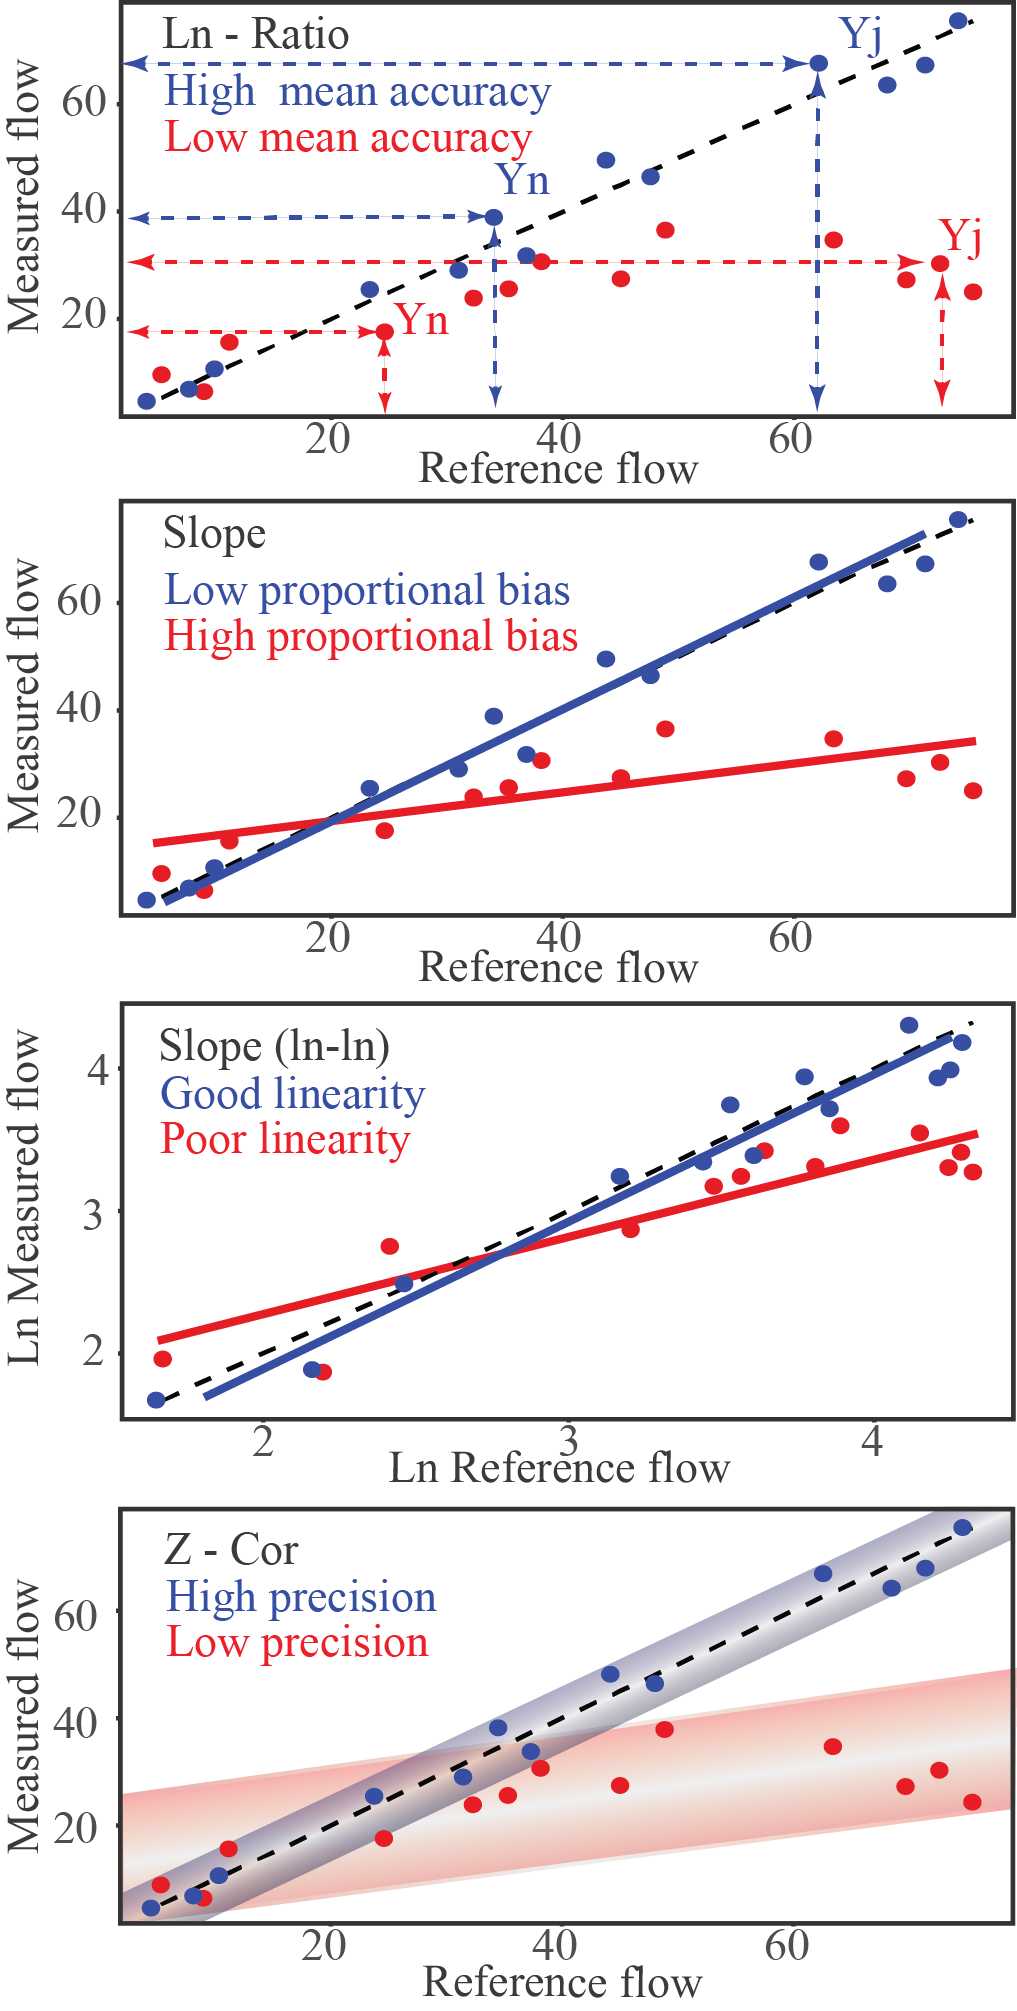
\includegraphics[width=0.55\linewidth]{figure/CH2/PLOTMETRICS} 

}

\caption[Graphical representation of the calibration performance metrics.]{Graphical representation of the calibration performance metrics used in the analyses. Each panel presents the same simulated calibration points, representing plausible data. Blue dots represent an accurate, unbiased, linear and precise calibration, while red dots represent an inaccurate, biased, non-linear and imprecise calibration.}\label{fig:ch2fig1}
\end{figure}
In the analysis of the absolute errors of sap flow measurements, we
calculated the Normalized Root Mean Square Error (NRMSE) for each
calibration (\(i\)) (Eq. 6), separately for SFD and SF methods, in order
to obtain the percentage of absolute error at the mean range of each
calibration (\(i\)).
\begin{equation}
NRMSE_i = \frac{(\sqrt \frac{\sum_{j=1}^{n} (measured_j-reference_j)^2}{n})_i\times 100}{range\;mean_i}
\end{equation}
Subsequently, from the NRMSE and the mean range of each calibration, we
fitted a linear model for each method allowing to quantify the absolute
error (RMSE) at a given sap flow and also to obtain a RMSE at a
reference flow (cf.~section 2.3).\par

\subsection{Statistical analyses}\label{statistical-analyses}

All the analyses were performed using linear mixed-effects models (LMM)
with the package lmer (Bates, Mächler, Bolker, \& Walker (2015)).
Least-square means were estimated with package lsmeans (Lenth (2016))
and used to summarise the effects of fixed factors and to test contrasts
among predictions. In all models, we used the variables Study and
Species as partially crossed random effects (Schielzeth \& Nakagawa
(2013)), as we are interested in taking into account the variability
associated with study and species, and also to analyze within- and
between-group variability. We used Study as we expect experimental
variability between researchers or laboratories, and Species because
calibration performance has been reported to vary across species (S.
Fuchs et al. (2017); D. Smith \& Allen (1996); Steppe et al. (2015)).
For each model, \(R^2_m\) and \(R^2_c\) (marginal and conditional
coefficients of determination, respectively) based on Nakagawa \&
Schielzeth (2013) were calculated using the function r.squaredGLMM of
the package MuMIn (Barton (2017)) in R. Intraclass Correlation
Coefficients (ICC) were also calculated for the random factors to
quantify the proportion of variance within and among groups (low ICC
implies high intra-group variability).\par

In a first analysis, we were interested in assessing the differences in
calibration metrics (Ln-Ratio, Slope, Slope (ln-ln), Z-Cor) between
different families of methods (Family: Pulse, Dissipation, Balance and
Field methods), because methods within a family share similar physical
principles. We also analyzed differences between individual methods with
a sufficient sample size (Method: CHP, T-max, HR, HFD, SHB, TD, TTD). As
the calibration material determines, to a large extent, the experimental
conditions, we also included this variable in our models (Material:
whole plants, whole plants without roots or cut stem segments). For the
analysis of absolute errors of sap flow measurements, we modelled NRMSE
as a function of Method and the Mean Range of SFD (or SF for Balance
methods) in each calibration, as well as their interaction. We used the
same random structure as in previous models.\par 

Finally, we assessed how each calibration metric depended on Wood
Density and Wood Porosity. A first model included all methods available,
with Method interacting with Wood Density as predictors. In order to
test Wood Porosity effects, we fitted separate models for CHP and TD
calibrations, as these two methods were the only ones that had enough
data (\textgreater{} 5 calibrations) for more than one type of porosity.
Separate models were needed because not all wood porosity types were
represented for all methods. In both models we also included Material as
an explanatory cofactor, and the same random structure as in the first
analysis explained above.\par

\section{Results}\label{results}

Most of the published calibrations were performed with Pulse and
Dissipation methods (Table 1.1). In particular, 61\% of the total number
of the properly applied calibrations were conducted using TD or CHP,
followed by HFD and HR. SHB, T-max and TTD methods were less
represented, with 8 -- 14 calibrations each. The metrics extracted from
the raw calibrations were highly variable within methods (Fig. 1.2).
Calibration metrics often followed a quasi-normal distribution, but in
most cases distributions were truncated or skewed, particularly for
methods with fewer calibrations (Fig. 1.2).\par
\begin{table}

\caption[Analysis summary for the different methods and families.]{\label{tab:Ch1T1}Analysis summary for the different methods and families of methods obtained from the LMM models (least-squares means). We provide the four dimensionless metrics: the Ln-ratio as a measure of accuracy, the accuracy deviation calculated as the exponential of the Ln-ratio minus one multiplied by 100, the Slope to characterize the proportional bias, the slope of the ln-ln-relationship, Slope (ln-ln), as a measure of linearity, and Z Pearson’s correlation (Z-Cor) to describe overall precision; n: number of calibrations; studies: number of studies of each method; species: number of different species; r is the correlation calculated as the tanh of Z-Cor.}
\resizebox{\linewidth}{!}{
\fontsize{6}{8}\selectfont
\begin{tabular}[t]{llllll>{\raggedright\arraybackslash}p{2cm}llll}
\toprule
Method & Family & n & studies & species & Ln-Ratio & Accuracy deviation \% & Slope & Slope (ln-ln) & Z-Cor & r\\
\midrule
CHP & Pulse & 63 & 16 & 21 & 0.133 & 14.225 & 0.887 & 0.783 & 1.837 & 0.950\\
T-max & Pulse & 11 & 5 & 6 & -0.053 & -5.162 & 0.614 & 0.697 & 1.755 & 0.942\\
HR & Pulse & 23 & 6 & 7 & -0.145 & -13.498 & 0.845 & 0.841 & 2.000 & 0.964\\
HFD & Field & 57 & 3 & 4 & -0.073 & -7.040 & 0.901 & 0.782 & 2.378 & 0.983\\
SHB & Balance & 8 & 5 & 6 & -0.242 & -21.494 & 0.847 & 0.967 & 2.287 & 0.980\\
TD & Dissipation & 115 & 18 & 35 & -0.519 & -40.488 & 0.683 & 1.066 & 1.711 & 0.937\\
TTD & Dissipation & 14 & 2 & 6 & -0.493 & -38.921 & 0.669 & 0.985 & 1.464 & 0.899\\
all & Pulse & 97 & NA & 30 & 0.012 & 1.167 & 0.844 & 0.787 & 1.874 & 0.954\\
all & Field & 57 & NA & 4 & -0.008 & -0.820 & 0.896 & 0.762 & 2.322 & 0.981\\
all & Balance & 8 & NA & 6 & -0.244 & -21.650 & 0.854 & 0.972 & 2.294 & 0.980\\
all & Dissipation & 129 & NA & 37 & -0.464 & -37.153 & 0.681 & 1.052 & 1.666 & 0.931\\
\bottomrule
\end{tabular}}
\end{table}
\begin{figure}[hbt!]

{\centering 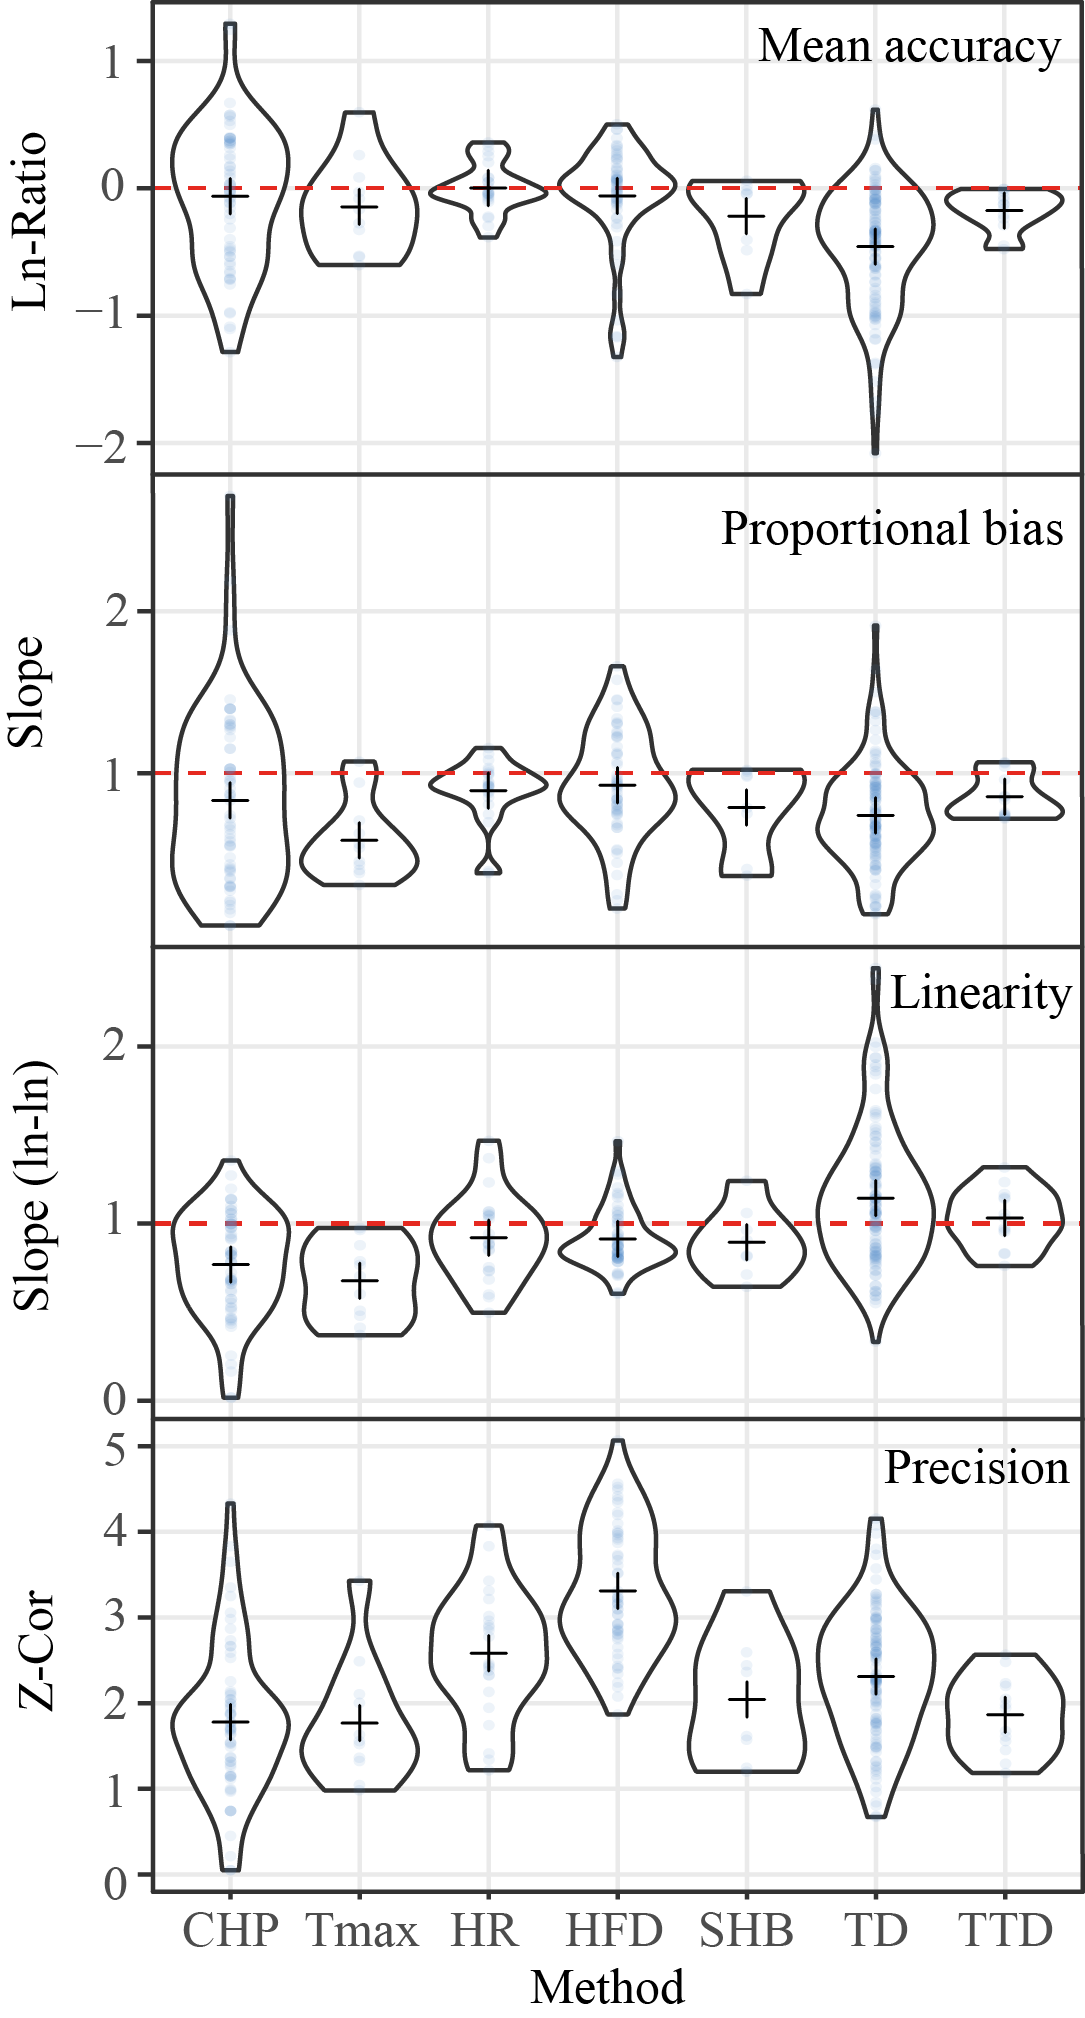
\includegraphics[width=0.55\linewidth]{figure/CH2/Distribution-metrics-orderedV4} 

}

\caption[Distribution of the calibration performance metrics for each method.]{Distribution of the calibration performance metrics for each method. Dots represents the value of each individual calibration metric. Crosses represent the average of the metric for each method. Horizontal, dashed lines specify reference, perfect calibration values for a given metric.}\label{fig:ch2fig2}
\end{figure}
\subsection{Calibration performance compared among methods and families
of
methods}\label{calibration-performance-compared-among-methods-and-families-of-methods}

The average accuracy deviation across sap flow methods (properly
applied) ranged between 14.2\% for CHP and -40.5\% for TD (Table 1.1).
There were significant differences in accuracy (Ln-Ratio) among families
of methods and for methods but not for calibration materials (Fig. 1.3).
The Dissipation family in general and the TD and TTD methods in
particular were the only cases for which the Ln-Ratio was significantly
different from 0 (p\textless{}0.001) (Fig. 1.3), indicating systematic
bias (underestimation).\par

Proportional bias, estimated by Slope, varied among methods and families
of methods (p\textless{}0.01). Among families, Dissipation methods
showed a significantly smaller Slope than Pulse and Field methods (Fig.
1.3(a)), which was largely driven by the low value of TD (Fig. 1.3(b)).
Also, both Pulse and Dissipation families had slopes significantly
different from 1 (p\textless{}0.01 and p\textless{}0.001, respectively),
but only the slope of the TD method was significantly lower than 1
(p\textless{}0.001) (Fig. 1.3). As for the effects of calibration
material, calibrations made with whole plants had a significant
proportional bias (Slope \textless{} 1, p\textless{}0.001) (Fig. 1.3).
\begin{figure}[p]

{\centering 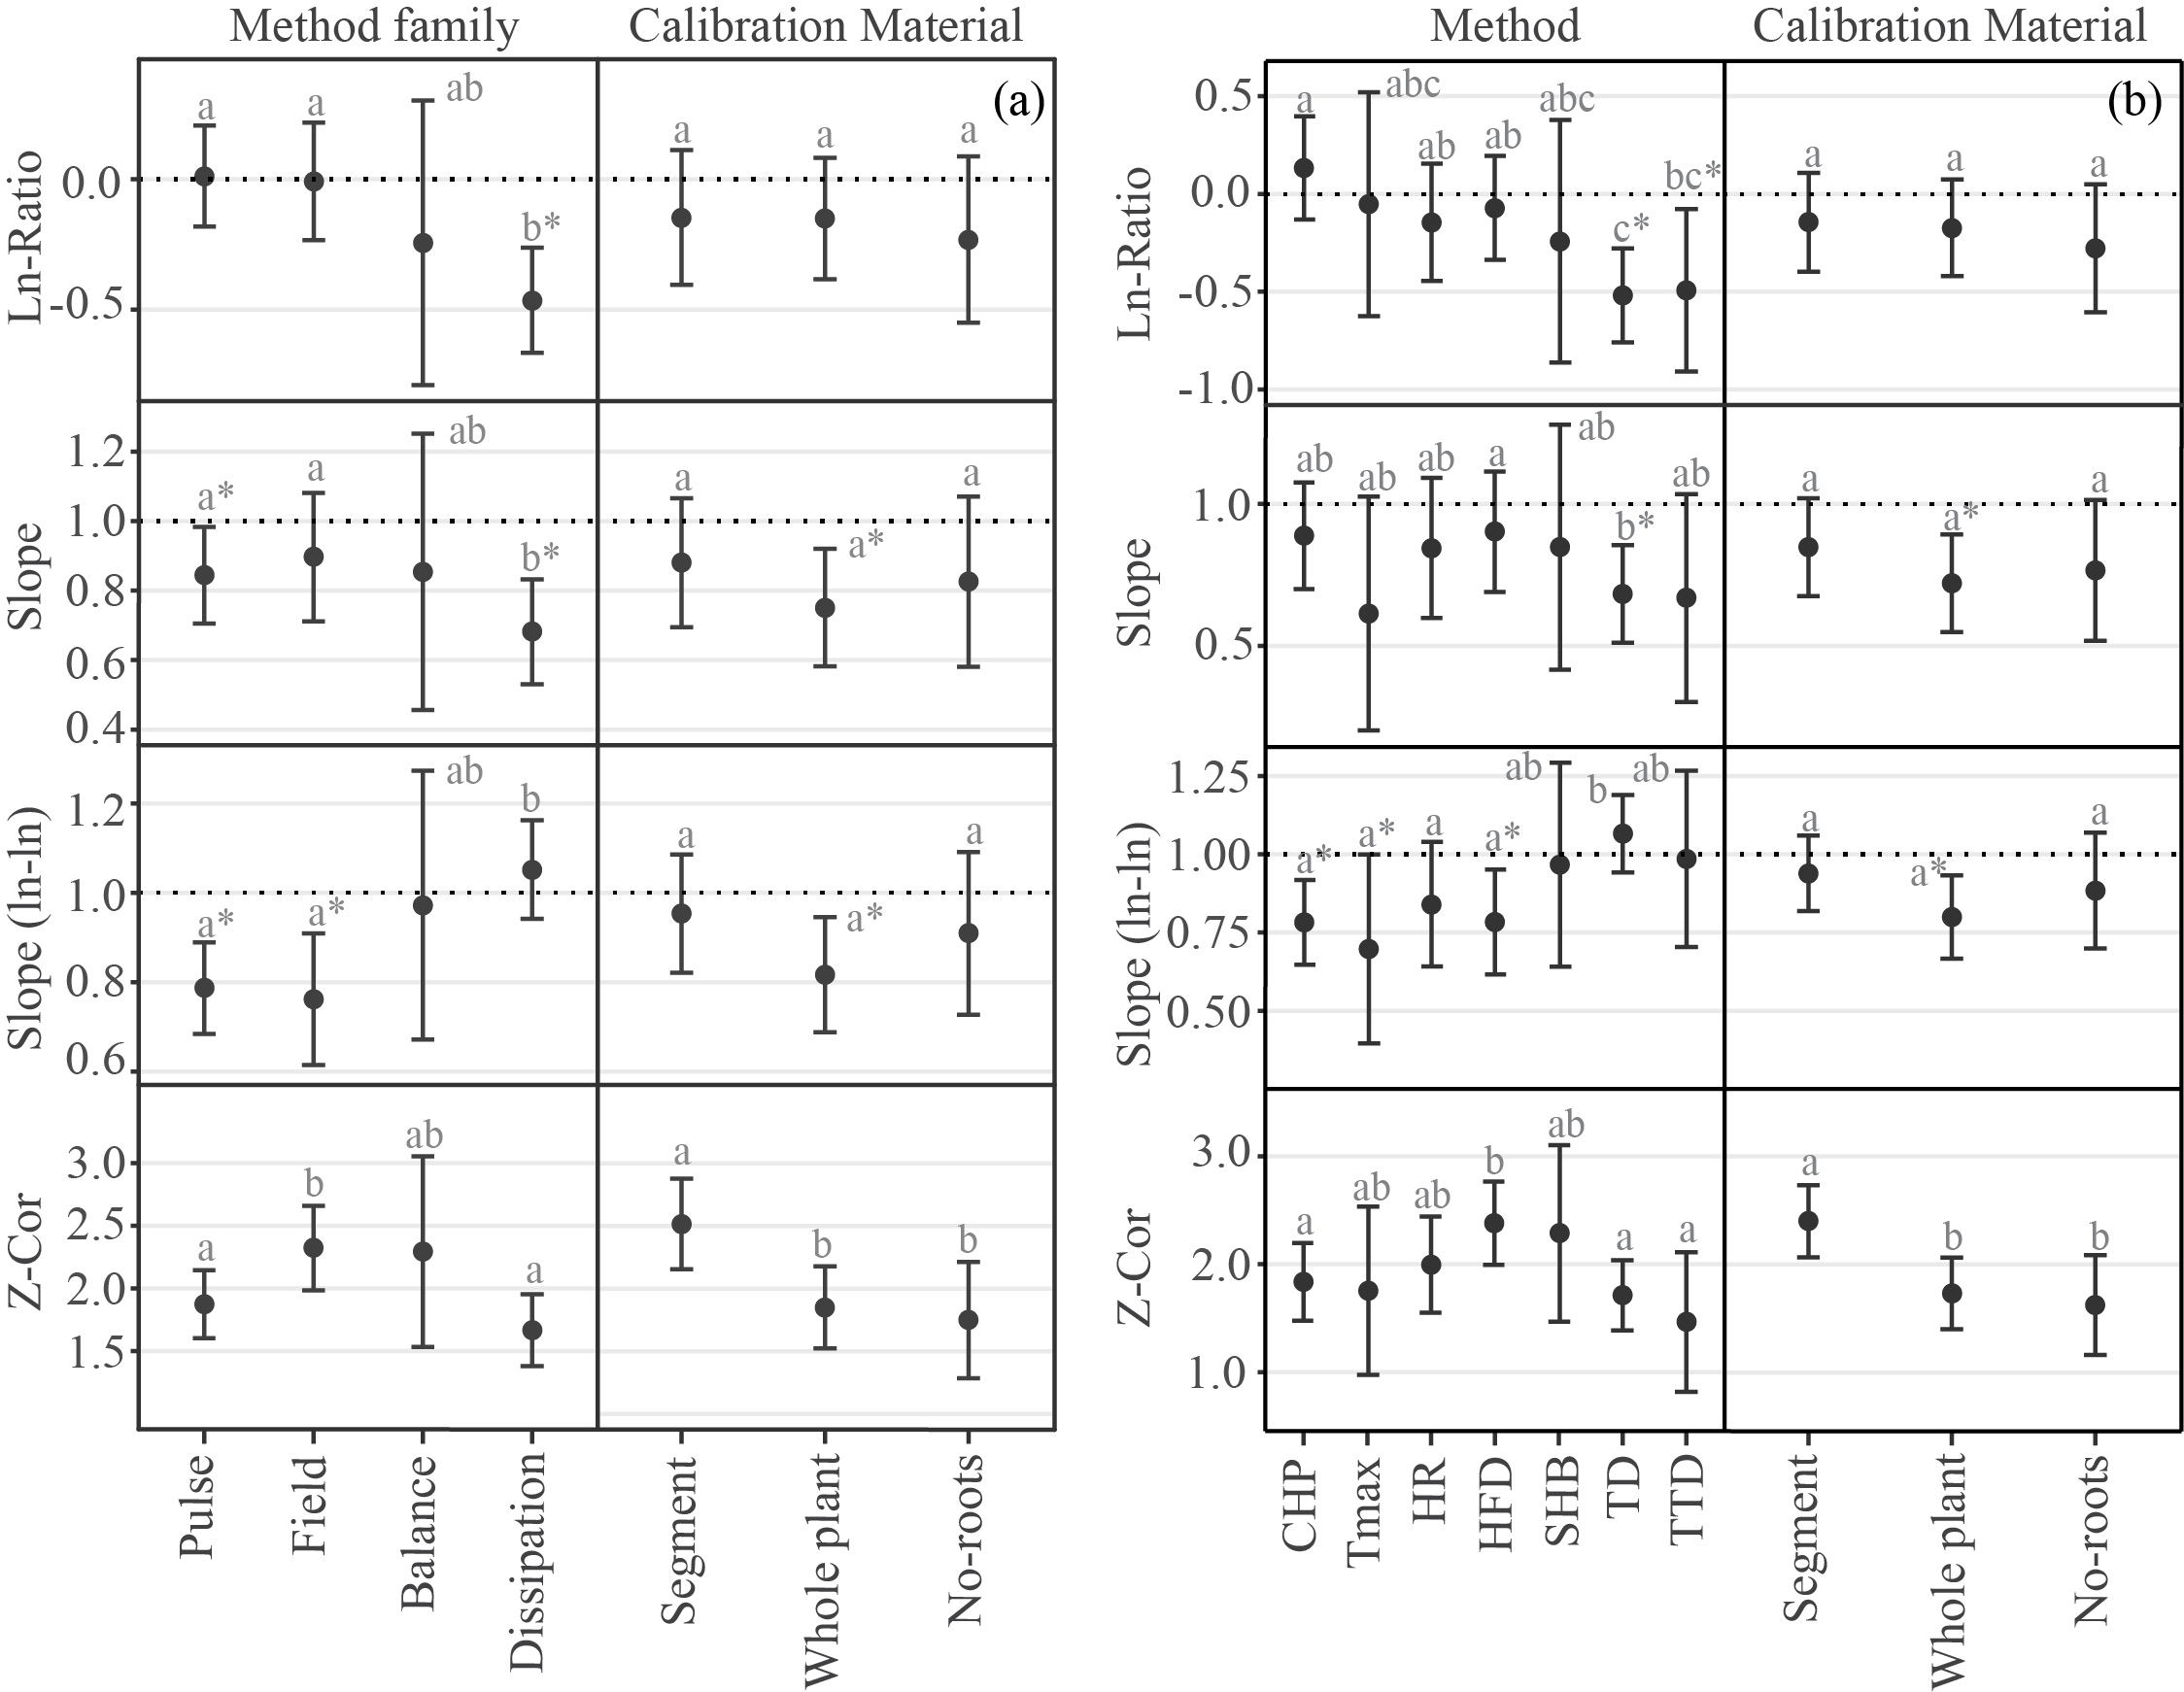
\includegraphics[width=1\linewidth]{figure/CH2/FAMILYMETHODS} 

}

\caption[Predictions of the LMM models of the four calibration metrics.]{Predictions of the LMM models calculated from least-squares means of the four calibration metrics (Ln-Ratio as a proxy for mean accuracy, Slope for proportional bias, Slope (ln-ln) for linearity and Z-Cor for precision) for (a) different families of sap flow methods or for (b) different sap flow methods and for different calibration materials (Segment: stem segment; Whole plant: whole plant on a container or lysimeter; No-roots: whole plant without roots). 95\% confidence intervals of the estimates are also shown. Different letters indicate significant differences between factors levels evaluated with Tukey's test. Horizontal, dotted lines indicate reference, perfect calibration values for a given metric. Asterisks (*) indicate significant departure from those reference values.}\label{fig:ch2fig3}
\end{figure}
Calibration linearity, as denoted by Slope (ln-ln), varied across
methods and families of methods (p\textless{}0.001). We observed higher
values of Slope (ln-ln) for the TD method compared to CHP, T-max, HR and
HFD. Consistently, the Dissipation family in general also had a higher
Slope (ln-ln) than the Pulse and Field families (Fig. 1.3). CHP, T-max
and HFD (and Pulse and Field methods in general) had a Slope (ln-ln)
significantly lower than 1 (Table 1.1 and Fig. 1.3(b)), indicating a
convex relationship between reference and measured flow. Calibrations
performed with whole plants suffered from lack of linearity, indicated
by Slope (ln-ln) significantly lower than 1 (Fig. 1.3).\par

Precision (Z-Cor) was explained by both method and calibration material.
The HFD method (and Field methods in general) provided significantly
higher precision than either Pulse or Dissipation methods (particularly
CHP, TD and TTD) (Table 1.1 and Fig. 1.3(b)). Calibrations performed on
stem segments provided higher precision than those conducted on whole
plants (with or without roots) (Fig. 1.3).\par

In all the previous models, little variability was explained by species
(\(\tau 00\), species), relative to the higher variability associated to
Study, particularly for the Ln-Ratio and Z-Cor models (\(\tau 00\),
study, Table A3). This is consistent with the low ICC values observed
for the species factor, indicating that there is more variability within
than among species (Table A3).\par

In addition, the analysis of the normalized absolute error for the
different methods showed that NRMSE decreased linearly with increasing
measured sap flow in CHP, HFD and TTD methods and increased for T-max,
SHB and TD (Table 1.2 and Fig. A2). For HR the increase in NRMSE with
measured sap flow was not significant. For all the methods that measure
SFD, the absolute error at a typical flow of 25 cm3 cm-2 h-1 ranged
between 6.3 cm3 cm-2 h-1 for CHP and 10.7 cm3 cm-2 h-1 for the TTD
method (Table 1.2).\par
\begin{table}[!h]

\caption[Error analysis of different sap flow methods.]{\label{tab:Ch2T2}Error analysis of different sap flow methods. The normalized root mean square error (NRMSE) is modelled as a function of method and the mean flow range for each calibration (and their interaction) using a LMM model with the same random structure as the main models (cf. section 2.3). $\beta_0$ and $\beta_1$ are the corresponding intercepts and slopes, respectively ($\beta_0$ expressed as \% NRMSE; $\beta_1$ expressed as \% NRMSE per change in $cm^3$ $cm^{-2}$ $h^{-1}$ for SFD or as \% NRMSE per change in $cm^3$ $h^{-1}$ for SF). This linear model, was also used to calculate a reference NRMSE at a sap flux equivalent to the percentile 50 of the range of the data in the calibrations (SFD: 25 $cm^3$ $cm^{-2}$ $h^{-1}$; SF: 1300 $cm^3$ $h^{-1}$). The expected NRMSE and RMSE (in brackets, in $cm^3$ $cm^{-2}$ $h^{-1}$, except for SHB that is in $cm^3$ $h^{-1}$) at a typical flow are also given.}
\centering
\fontsize{10}{12}\selectfont
\begin{tabular}[t]{cccc}
\toprule
\multicolumn{1}{c}{ } & \multicolumn{3}{c}{NRMSE} \\
\cmidrule(l{3pt}r{3pt}){2-4}
Method & $\beta_0$\; \% & $\beta_1$ & reference NRMSE (and RMSE)\\
\midrule
CHP & 27.03*** & -0.08*** & 25.04\% (6.26)\\
T-max & 31.56. & 0.25*** & 37.83\% (9.46)\\
HR & 9.38 & 0.81 & 29.59\% (7.40)\\
HFD & 30.33*** & -0.12*** & 27.45\% (6.86)\\
SHB & 14.85 & 0.02*** & 42.95\% (558.36)\\
TD & 34.93*** & 0.10*** & 37.31\% (9.33)\\
TTD & 44.04*** & -0.04*** & 42.94\% (10.73)\\
\bottomrule
\multicolumn{4}{l}{\textsuperscript{} Statistical significant levels: "." p<0.1 ; "*" p<0.05; "**" p<0.01; "***"}\\
\multicolumn{4}{l}{p<0.001.}\\
\end{tabular}
\end{table}
\subsection{Influence of wood traits}\label{influence-of-wood-traits}

We did not find any significant influence of wood density on accuracy
and linearity metrics (Fig. 1.4). Nonetheless, we observed a negative
effect of wood density on proportional bias of HFD and TD calibrations
(p\textless{}0.05 and p\textless{}0.1, respectively). In addition, a
significant positive effect of wood density on the precision of HFD
measurements was observed (p\textless{}0.001), indicating that the
higher the wood density, the higher the precision (Fig. 1.4).\par

We did not find any significant difference among wood porosity types in
calibration metrics for studies using the TD or CHP methods.
Nevertheless, the non-linearity (Slope (ln-ln) \textless{} 1) observed
in general for the CHP method (Fig. 1.3(b)) was only significant for
species with diffuse-porous wood, not for conifer species (Table
1.3).\par
\begin{figure}[hbt!]

{\centering 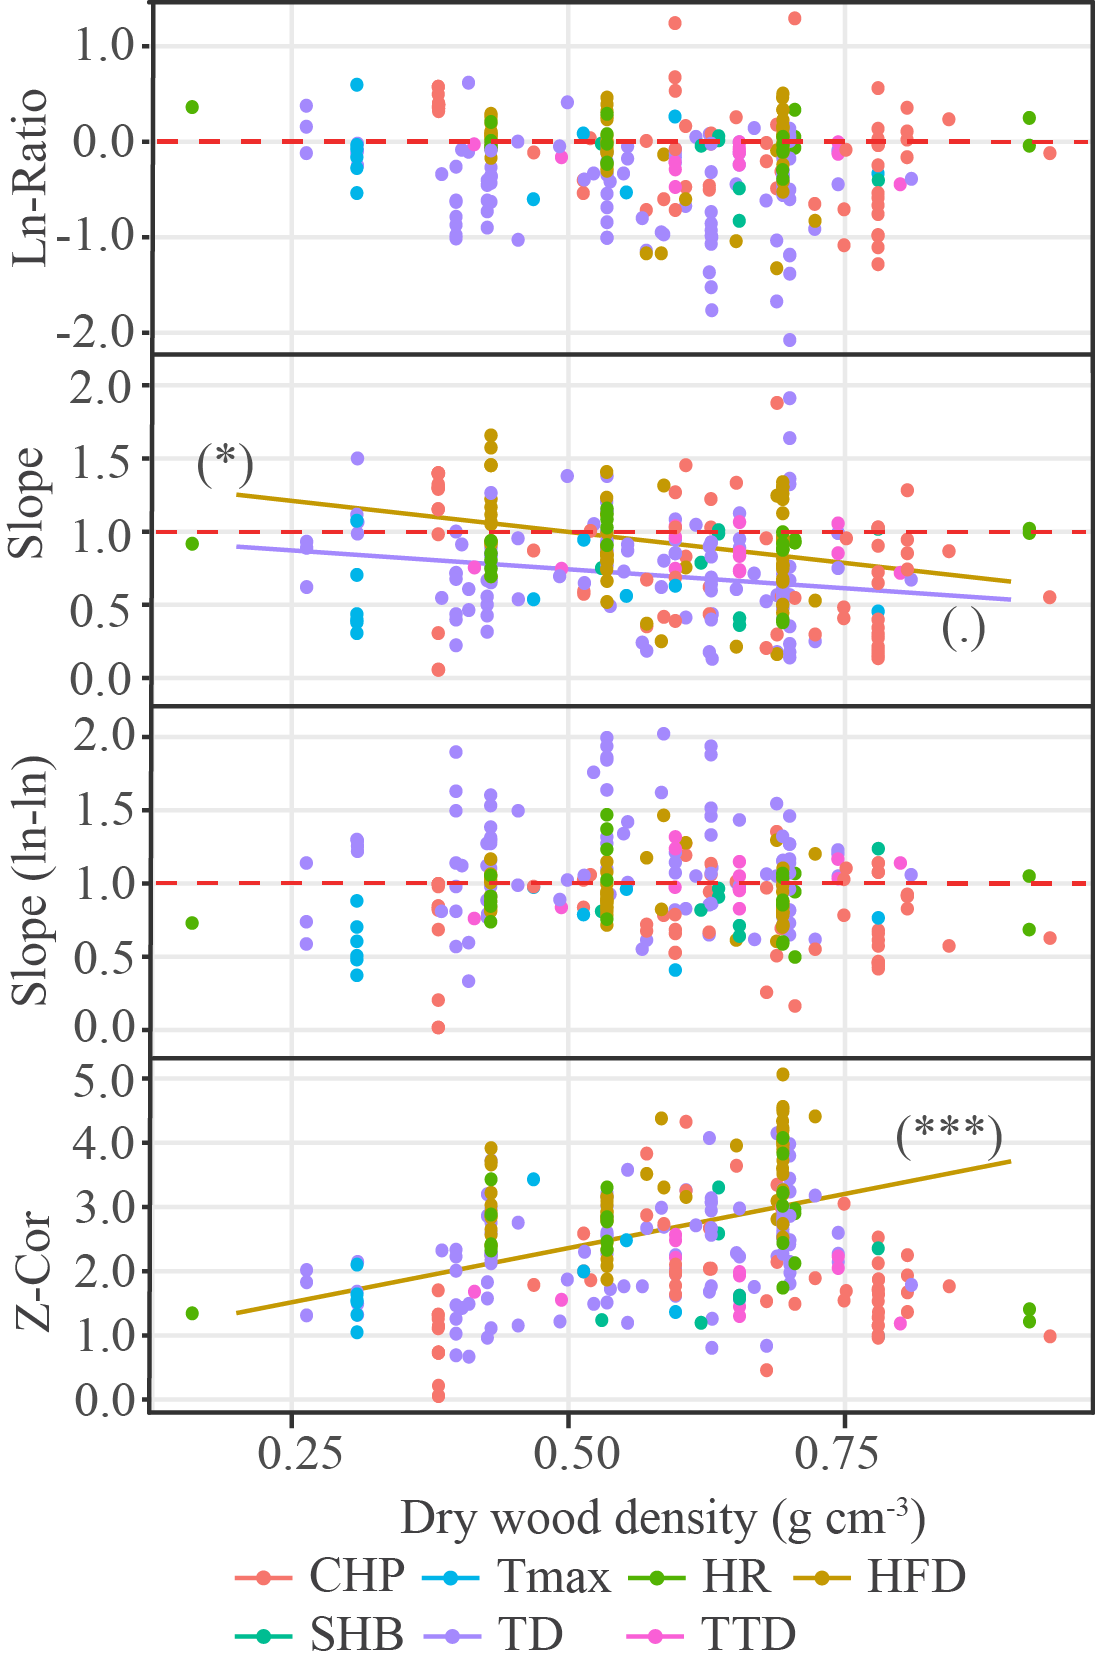
\includegraphics[width=0.55\linewidth]{figure/CH2/DENSITY} 

}

\caption[Relationship between the four calibration performance and wood density, for different sap flow methods.]{Relationship between the four calibration performance metrics (Ln-Ratio as a proxy for accuracy, Slope for proportional bias, Slope (ln-ln) for linearity, and Z-Cor for precision) and wood density, for different sap flow methods. Horizontal, dashed red lines indicate reference, perfect calibration values for a given metric. Regression lines are shown for significant effects only, and the corresponding level of significance (p-value: <0.1: (.), <0.05: (*), < 0.01: (**), < 0.001: (***)) is also reported }\label{fig:ch2fig4}
\end{figure}
\begin{table}

\caption[Least-squares means and 95\% CI calculated from the LMM models testing the effect of different wood porosity types]{\label{tab:Ch2T3}Least-squares means and 95\% CI calculated from the LMM models testing the effect of different wood porosity types (Wood porosity) on sap flow calibration performance metrics (Ln-Ratio as a proxy for accuracy, Slope for proportional bias, Slope (ln-ln) for linearity, and Z-Cor for precision) for CHP and TD methods. No differences were detected among wood anatomies. Significance levels indicate departure from an ideal calibration (Ln-Ratio = 0; Slope = 1; Slope (ln-ln) = 1)}
\centering
\resizebox{\linewidth}{!}{
\fontsize{6}{8}\selectfont
\begin{tabular}[t]{c>{\centering\arraybackslash}p{1.5cm}ccccc}
\toprule
\multicolumn{1}{c}{ } & \multicolumn{1}{c}{ } & \multicolumn{1}{c}{ } & \multicolumn{1}{c}{Accuracy} & \multicolumn{1}{c}{Proportional bias} & \multicolumn{1}{c}{Linearity} & \multicolumn{1}{c}{Precision} \\
\cmidrule(l{3pt}r{3pt}){4-4} \cmidrule(l{3pt}r{3pt}){5-5} \cmidrule(l{3pt}r{3pt}){6-6} \cmidrule(l{3pt}r{3pt}){7-7}
Method & Wood porosity & n & Ln-Ratio & Slope & Slope (ln-ln) & Z-Cor\\
\midrule
CHP & diffuse & 48 & -0.055 [-0.370 , 0.259] & 0.795 [0.557 , 1.033]. & 0.799 [0.671, 0.927] \*\* & 1.980 [1.729 , 2.231]\\
CHP & conifers & 15 & 0.066 [-0.603 , 0.734] & 1.043 [0.459 , 1.627] & 0.777 [0.469 , 1.085] & 1.381 [0.775 , 1.988]\\
TD & diffuse & 81 & -0.273 [-0.658 , 0.111] & 0.752 [0.491 , 1.014]. & 1.126 [0.917 , 1.336] & 1.672 [1.085 , 2.260]\\
TD & ring & 16 & -0.405 [-0.866 , 0.056]. & 0.743 [0.410 , 1.077]. & 0.984 [0.681 , 1.286] & 2.260 [1.572 , 2.947]\\
TD & conifers & 15 & -0.396 [-0.873 , 0.080]. & 0.808 [0.468 , 1.147] & 1.142[0.842 , 1.441] & 1.606 [0.892 , 2.321]\\
\bottomrule
\multicolumn{7}{l}{\textsuperscript{} Statistical significant levels: "." p<0.1 ; "*" p<0.05; "**" p<0.01; "***" p<0.001.}\\
\end{tabular}}
\end{table}
\section{Discussion}\label{discussion}

Our results show a large variability in the quality of sap flow
calibrations, even within the same sap flow method (Fig. 1.2),
highlighting the large variability among and even within studies. This
implies that, even if methods are properly applied (as defined in
section 2.1), sap flow measurements can still produce biased estimates
of water transport rates in plants, and these errors will need to be
considered in quantitative analyses based on this type of measurements.
On average, however, all sap flow methods assessed here produced results
that may be acceptable for qualitative use in most applications, as
shown by the typical high correlation between measured and reference
values (r \textgreater{} 0.89 for all methods and method families, Table
1.1). For quantitative use, no method appears to be suitable for all
experimental contexts, and researchers need to consider both the
inherent limitations of the methods and the need to perform
study-specific calibrations (see Implications and recommendations, Table
1.4).\par

\subsection{Sap flow measurement errors across methods and
methodological
families}\label{sap-flow-measurement-errors-across-methods-and-methodological-families}

A relatively small part of the total variability in the quality of
calibrations is related to methods and families of methods and, to a
lesser extent, to the calibration material (fixed effects explain 8 --
28\% of the variability in calibration metrics; see \(R^2_m\) values in
Table A3). Despite the high variability within methods, we detected
significant differences between methods. Dissipation methods were the
only methods for which accuracy was significantly lower than expected
for an ideal calibration. This is consistent with previous reports
(Braun \& Schmid (1999); S. E. Bush, Hultine, Sperry, Ehleringer, \&
Phillips (2010); Caterina, Will, Turton, Wilson, \& Zou (2014);
({\textbf{???}}); de Oliveira Reis, Campostrini, Sousa, \& Silva (2006);
S. Fuchs et al. (2017); Ping Lu \& Chacko (1998); McCulloh et al.
(2007); Montague \& Kjelgren (2006); Rubilar, Hubbard, Yañez, Medina, \&
Valenzuela (2017); Steppe, De Pauw, Doody, \& Teskey (2010); Taneda \&
Sperry (2008); Uddling, Teclaw, Pregitzer, \& Ellsworth (2009)) and our
synthesis confirms that most of the individual TD and all TTD
calibrations underestimate sap flow systematically (Fig. 1.5).
Interestingly, however, other studies have found the opposite result
(Cain (2009); K. R. Hultine et al. (2010); P Lu (2002); Sperling et al.
(2012); Sun, Aubrey, \& Teskey (2012)) and simulation models (Hölttä,
Linkosalo, Riikonen, Sevanto, \& Nikinmaa (2015); Wullschleger et al.
(2011)) suggest that it is difficult to state a priori whether TD will
over- or underestimate flow, as the measurements obtained are highly
dependent on wood properties and on flux conditions. Our results show
that, globally, the conditions leading to underestimation are more
frequent and support the existence of a proportional bias underlying
this systematic underestimation by TD (Fig. 1.3). It must be also noted,
however, that Dissipation methods have been tested against a much wider
range of flow conditions compared to the rest of the methods (Fig. 1.5,
Fig.6).\par
\begin{table}[!h]

\caption[Synthesis of the potential sources of error and use adequacy for each method.]{\label{tab:Ch2T4}Synthesis of the potential sources of error and use adequacy for each method. Crosses indicates that the method is sensitive to the respective source of error (updated from Vandegehuchte and Steppe, 2013). Methods are classified according to their use effectiveness under different flow conditions: dark grey, light grey and white indicate highly, partially and no recommended use, respectively. When assessing use adequacy for high/low flows, dark and light gray indicate a Normalized Root Mean Square Error (NRMSE) less than a 22\% and a 44\%, respectively, calculated with the NRMSE model (Table 1.2). In Absolute flows use recommendation, dark grey shows methods with both accuracy (Ln-Ratio) and proportional bias (Slope) not significantly different from a perfect calibration. In Relative flows use recommendation, dark grey shows methods with linearity (Slope (ln-ln)) not significantly different from a perfect calibration and with reasonable precision. Potentiality of measuring small stems diameters (< 125mm) is also reported.}
\centering
\fontsize{10}{12}\selectfont
\begin{threeparttable}
\begin{tabular}[t]{cccccccccccccccc}
\toprule
\multicolumn{1}{c}{ } & \multicolumn{9}{c}{Potential source of measure error} & \multicolumn{6}{c}{Effectiveness in measuring} \\
\cmidrule(l{3pt}r{3pt}){2-10} \cmidrule(l{3pt}r{3pt}){11-16}
\rotatebox{90}{\em{Method}} & \rotatebox{90}{\em{Wounding}} & \rotatebox{90}{\em{Radial velocity profile}} & \rotatebox{90}{\em{Wood properties}} & \rotatebox{90}{\em{Natural thermal gradients}} & \rotatebox{90}{\em{Sensor installation}} & \rotatebox{90}{\em{Sensor design}} & \rotatebox{90}{\em{Baselining}} & \rotatebox{90}{\em{Power input}} & \rotatebox{90}{\em{Pulse length}} & \rotatebox{90}{\em{Reverse flows}} & \rotatebox{90}{\em{Low flows*}} & \rotatebox{90}{\em{High flows*}} & \rotatebox{90}{\em{Absolute flows}} & \rotatebox{90}{\em{Relative flows}} & \rotatebox{90}{\em{Small stems}}\\
\midrule
CHP & x & x & x & x & x &  &  &  & x & \multicolumn{1}{c}{\cellcolor[HTML]{FFFFFF}{\textcolor[HTML]{FFFFFF}{0}}} & \multicolumn{1}{c}{\cellcolor[HTML]{BBBBBB}{\textcolor[HTML]{BBBBBB}{1}}} & \multicolumn{1}{c}{\cellcolor[HTML]{999999}{\textcolor[HTML]{999999}{2}}} & \multicolumn{1}{c}{\cellcolor[HTML]{999999}{\textcolor[HTML]{999999}{2}}} & \multicolumn{1}{c}{\cellcolor[HTML]{FFFFFF}{\textcolor[HTML]{FFFFFF}{0}}} & \multicolumn{1}{c}{\cellcolor[HTML]{FFFFFF}{\textcolor[HTML]{FFFFFF}{0}}}\\
T-max & x & x & x &  & x &  & x &  &  & \multicolumn{1}{c}{\cellcolor[HTML]{FFFFFF}{\textcolor[HTML]{FFFFFF}{0}}} & \multicolumn{1}{c}{\cellcolor[HTML]{BBBBBB}{\textcolor[HTML]{BBBBBB}{1}}} & \multicolumn{1}{c}{\cellcolor[HTML]{FFFFFF}{\textcolor[HTML]{FFFFFF}{0}}} & \multicolumn{1}{c}{\cellcolor[HTML]{999999}{\textcolor[HTML]{999999}{2}}} & \multicolumn{1}{c}{\cellcolor[HTML]{FFFFFF}{\textcolor[HTML]{FFFFFF}{0}}} & \multicolumn{1}{c}{\cellcolor[HTML]{FFFFFF}{\textcolor[HTML]{FFFFFF}{0}}}\\
HR & x & x & x &  & x &  &  &  &  & \multicolumn{1}{c}{\cellcolor[HTML]{999999}{\textcolor[HTML]{999999}{2}}} & \multicolumn{1}{c}{\cellcolor[HTML]{999999}{\textcolor[HTML]{999999}{2}}} & \multicolumn{1}{c}{\cellcolor[HTML]{FFFFFF}{\textcolor[HTML]{FFFFFF}{0}}} & \multicolumn{1}{c}{\cellcolor[HTML]{999999}{\textcolor[HTML]{999999}{2}}} & \multicolumn{1}{c}{\cellcolor[HTML]{999999}{\textcolor[HTML]{999999}{2}}} & \multicolumn{1}{c}{\cellcolor[HTML]{999999}{\textcolor[HTML]{999999}{2}}}\\
HFD & x & x &  & x & x & x & x & x &  & \multicolumn{1}{c}{\cellcolor[HTML]{999999}{\textcolor[HTML]{999999}{2}}} & \multicolumn{1}{c}{\cellcolor[HTML]{BBBBBB}{\textcolor[HTML]{BBBBBB}{1}}} & \multicolumn{1}{c}{\cellcolor[HTML]{999999}{\textcolor[HTML]{999999}{2}}} & \multicolumn{1}{c}{\cellcolor[HTML]{999999}{\textcolor[HTML]{999999}{2}}} & \multicolumn{1}{c}{\cellcolor[HTML]{FFFFFF}{\textcolor[HTML]{FFFFFF}{0}}} & \multicolumn{1}{c}{\cellcolor[HTML]{999999}{\textcolor[HTML]{999999}{2}}}\\
SHB &  &  &  & x &  &  & x & x &  & \multicolumn{1}{c}{\cellcolor[HTML]{999999}{\textcolor[HTML]{999999}{2}}} & \multicolumn{1}{c}{\cellcolor[HTML]{999999}{\textcolor[HTML]{999999}{2}}} & \multicolumn{1}{c}{\cellcolor[HTML]{FFFFFF}{\textcolor[HTML]{FFFFFF}{0}}} & \multicolumn{1}{c}{\cellcolor[HTML]{999999}{\textcolor[HTML]{999999}{2}}} & \multicolumn{1}{c}{\cellcolor[HTML]{999999}{\textcolor[HTML]{999999}{2}}} & \multicolumn{1}{c}{\cellcolor[HTML]{999999}{\textcolor[HTML]{999999}{2}}}\\
TD & x & x & x & x &  & x & x & x &  & \multicolumn{1}{c}{\cellcolor[HTML]{FFFFFF}{\textcolor[HTML]{FFFFFF}{0}}} & \multicolumn{1}{c}{\cellcolor[HTML]{BBBBBB}{\textcolor[HTML]{BBBBBB}{1}}} & \multicolumn{1}{c}{\cellcolor[HTML]{BBBBBB}{\textcolor[HTML]{BBBBBB}{1}}} & \multicolumn{1}{c}{\cellcolor[HTML]{FFFFFF}{\textcolor[HTML]{FFFFFF}{0}}} & \multicolumn{1}{c}{\cellcolor[HTML]{999999}{\textcolor[HTML]{999999}{2}}} & \multicolumn{1}{c}{\cellcolor[HTML]{FFFFFF}{\textcolor[HTML]{FFFFFF}{0}}}\\
TTD & x & x & x & x &  & x & x & x &  & \multicolumn{1}{c}{\cellcolor[HTML]{FFFFFF}{\textcolor[HTML]{FFFFFF}{0}}} & \multicolumn{1}{c}{\cellcolor[HTML]{FFFFFF}{\textcolor[HTML]{FFFFFF}{0}}} & \multicolumn{1}{c}{\cellcolor[HTML]{BBBBBB}{\textcolor[HTML]{BBBBBB}{1}}} & \multicolumn{1}{c}{\cellcolor[HTML]{FFFFFF}{\textcolor[HTML]{FFFFFF}{0}}} & \multicolumn{1}{c}{\cellcolor[HTML]{999999}{\textcolor[HTML]{999999}{2}}} & \multicolumn{1}{c}{\cellcolor[HTML]{FFFFFF}{\textcolor[HTML]{FFFFFF}{0}}}\\
\bottomrule
\end{tabular}
\begin{tablenotes}
\small
\item [*] (Low/High: SFD methods: <5 / >80 $cm^{3} cm^{-2} h^{-1}$; SF methods: <260 / >3900 $cm^3 h^{-1}$)
\end{tablenotes}
\end{threeparttable}
\end{table}
Calibration parameters of the TD method were originally considered to be
universal but subsequent studies have claimed that species-specific
calibrations are necessary to obtain correct sap flow measurements (S.
Fuchs et al. (2017); Ping Lu et al. (2004); Steppe et al. (2010)). For a
set of diffuse-porous species, using a pooled calibration also
substantially improved TD (but not HFD) performance compared to
measurements obtained with the original calibration (S. Fuchs et al.
(2017)). However, our results show that species in general and wood
porosity type in particular explain a small or even no proportion of the
variability in the calibrations (Table 1.3 and A3). This implies that
factors related to the experimental context and, possibly, to
intraspecific variability in wood properties (cf.~section 1.5.2) may
have a large contribution to overall uncertainty. Therefore, our results
suggest that calibration parameters for TD or HFD, obtained under
different experimental contexts, may not be generalizable to species
level, as also suggested by Fuchs et al. (2017).\par

In addition to Dissipation methods, Pulse methods also suffer
proportional bias, probably driven by overestimation at low flows,
although this was significant for T-max only (i.e.~positive intercepts
in linear models fitted to calibration data; Fig. 1.5 and 1.6 and A3).
It is well known that the equations of CHP and T-max cannot be solved at
sap flows close to 0, and the calibration intercepts observed here (Fig.
A3) are consistent with the detection thresholds reported for T-max
(\textasciitilde{}10 cm3 cm-2 h-1; Steve Green et al. (2003)) and CHP
(2-4 cm3 cm-2 h-1; T. M. Bleby, Burgess, \& Adams (2004); Steve Green et
al. (2003)). Our results confirm and generalize a previously reported
low-flow detectability problem for T-max (S. Green et al. (2009), Steve
Green et al. (2003); Vandegehuchte \& Steppe (2012b)), but we could not
confirm it for CHP as described before (Barrett et al. (1995); Becker
(1998); T. M. Bleby et al. (2004); Vandegehuchte \& Steppe (2012b)).
Despite overestimation at low flows, the average accuracy of CHP and
T-max is good, which implies that low-flow overestimations may be
compensated with underestimations at high flows. This is also shown by
the lack of linearity observed in both methods (Slope (ln-ln)
\textless{} 1; Fig. 1.3(b)).\par

Our analysis did not detect the saturation effect for the HR method at
high flows that has been reported elsewhere (T. Bleby, McElrone, \&
Burgess (2008); S. Green et al. (2009); Steppe et al. (2015)). This is
likely due to the fact that HR calibrations considered here include few
observations in the region where this overestimation occurs
(\textgreater{} \textasciitilde{}45 cm3 cm-2 h-1; Figs 5 and 6).
Moreover, the high variability in the calibrations probably precluded
detection of the saturation effect (Fig. 1.3 and 1.5) and of the
apparent trend of increasing NRMSE with sap flow range for HR (Table 1.3
and Fig. A2). A lack of linearity can also be observed for HFD,
consistent with the suggested tendency of this method to underestimate
at high flows (Vandegehuchte \& Steppe (2012c)).\par
\begin{figure}[p]

{\centering 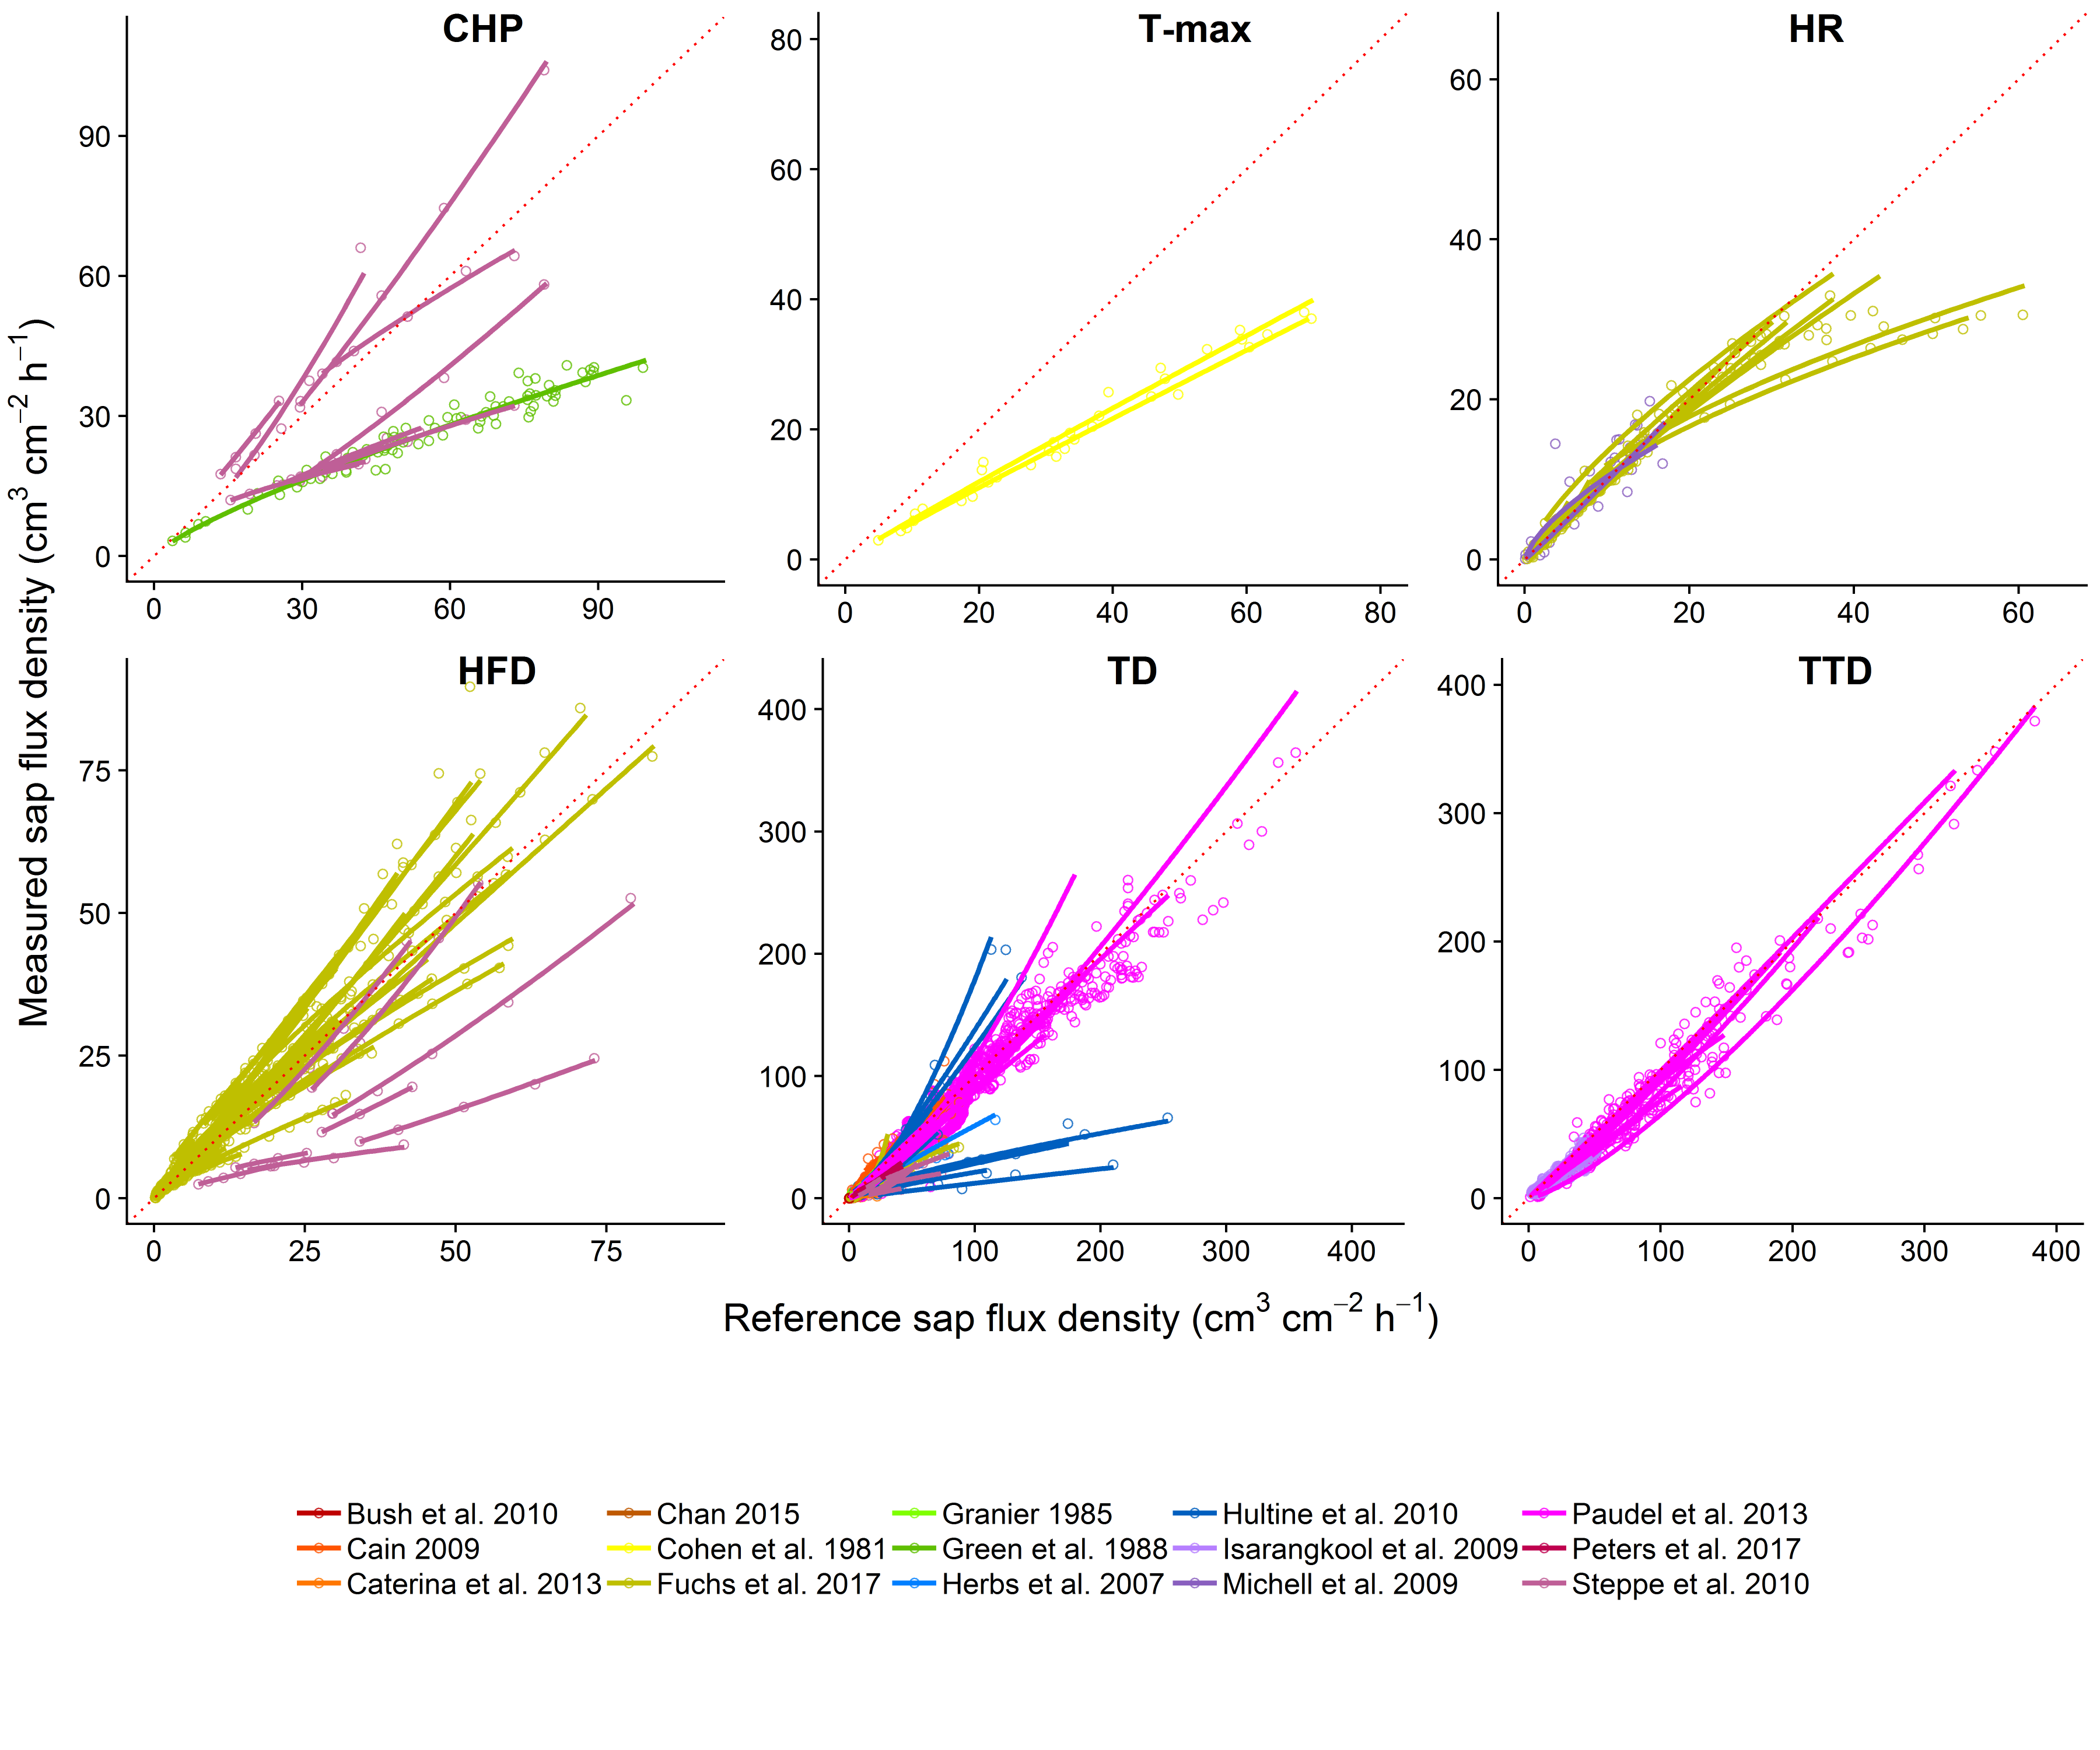
\includegraphics[width=1\linewidth]{figure/CH2/figure-density} 

}

\caption[Relationship between measured and reference sap-flux density (SFD) for different sap flow methods, studies and calibrations.]{Relationship between measured and reference sap-flux density (SFD) for different sap flow methods, studies and calibrations. The fits of ln-ln regressions (Eq. 4) for each calibration are also depicted. Different colors represent different studies that report results in sap-flux density units. Scales vary across panels to facilitate intra method comparison. The red dotted line indicates the 1:1 relationship.}\label{fig:ch2fig5}
\end{figure}
Despite the large variability in precision within methods, our results
show that calibrations performed with HFD give more precise results than
those conducted using the CHP, TD and TTD methods. Although this result
should be interpreted with care as it is based on 57 calibrations but
only from 3 studies, the higher precision observed with HFD could lie in
the second dimension included in the method, which could better capture
the effect of anisotropy of the wood structure. This would also be
consistent with the fact that SHB, a method that is assumed to integrate
sap flow variability within the stem, was the method with the second
highest precision on average, albeit precision was very variable for
this method (Fig. 1.3(b)).\par

We did not detect differences in accuracy, proportional bias or
linearity of the calibrations across calibration materials. However,
compared to an ideal calibration, we did find proportional bias and lack
of linearity in calibrations performed on whole plants, probably because
these calibrations use large scales whose sensitivity and resolution are
usually low, potentially affecting low-flow measurements and leading to
artefactual overestimation at low flows. Poor linearity may also be due
to non-linear changes in belowground hydraulic resistance as the sap
flow increases (J. Martínez-Vilalta, Korakaki, Vanderklein, \&
Mencuccini (2007)). In cut plants, we may have two opposite effects, as
cutting could eliminate belowground resistance (favoring flow) but add
resistance due to putative embolism formation after cutting. Similarly,
the higher precision of calibrations conducted on cut stems relative to
those conducted on whole plants (with and without roots), likely
reflects that cut stem calibrations are normally conducted in
laboratories with precision scales and under controlled conditions that
minimize experimental random errors.\par
\begin{figure}[p]

{\centering 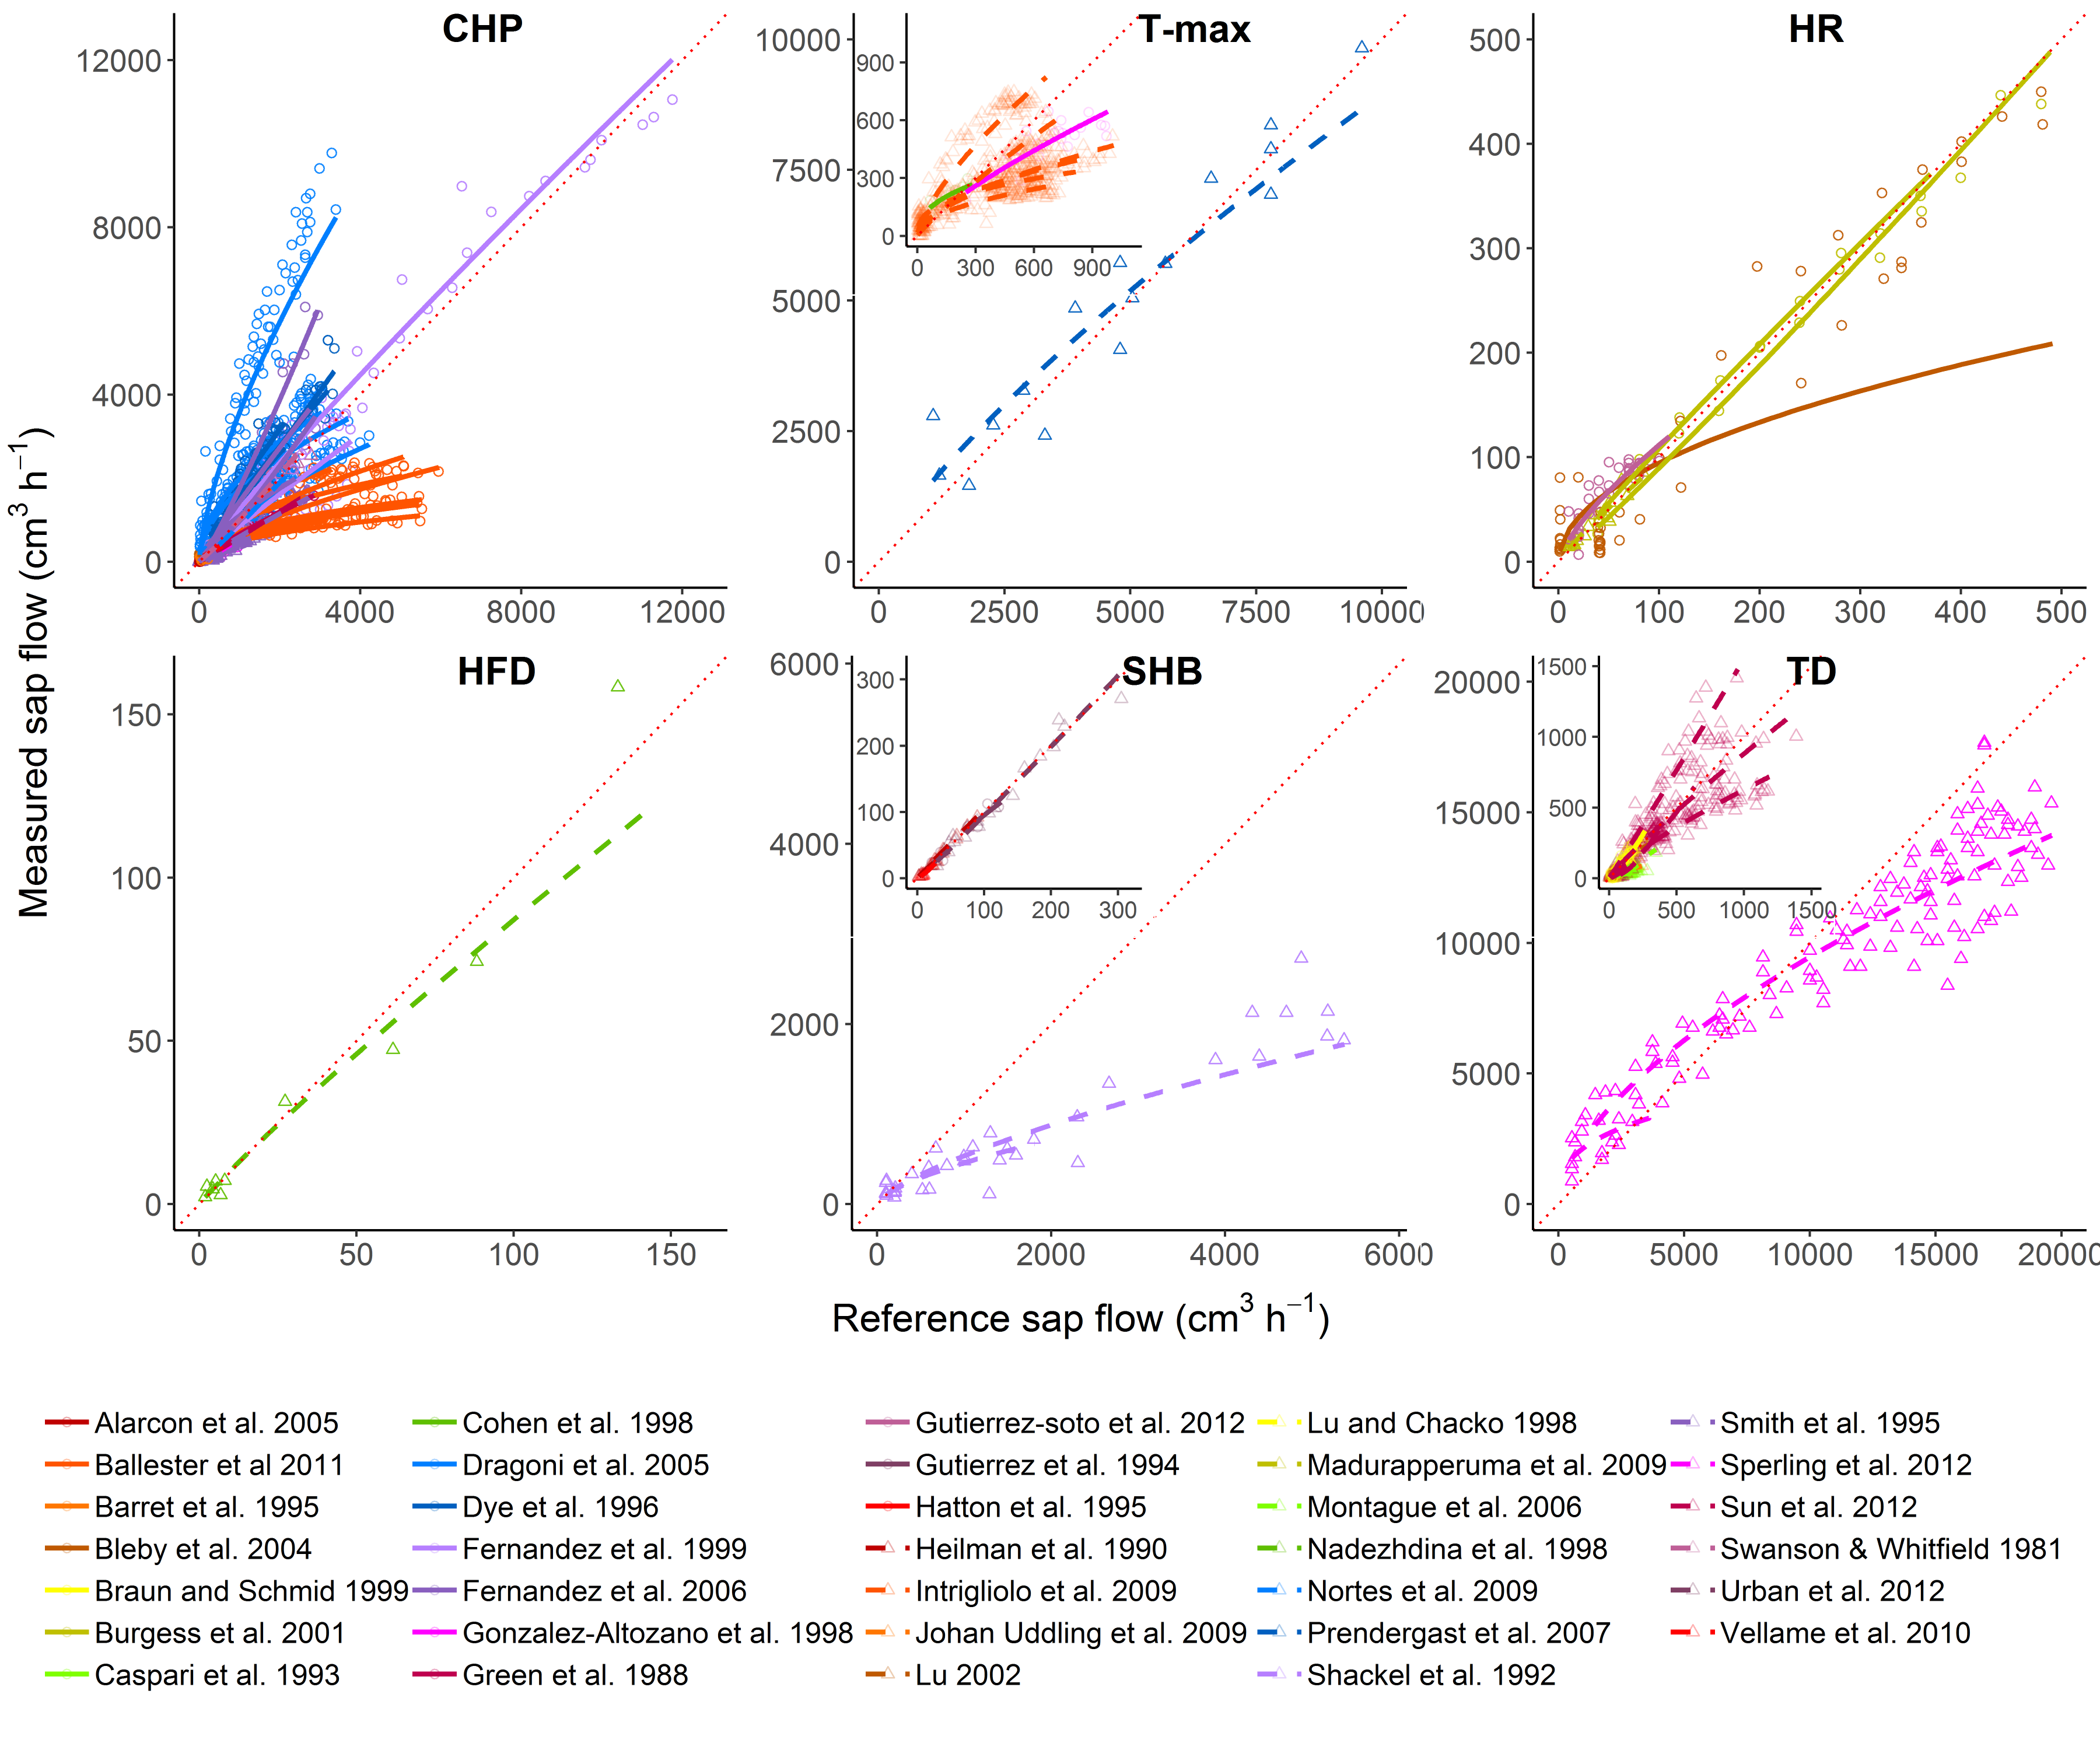
\includegraphics[width=1\linewidth]{figure/CH2/figure-totalflow} 

}

\caption[Relationship between measured and reference sap flow (SF) for different sap flow methods, studies and calibrations.]{Relationship between measured and reference sap flow (SF) for different sap flow methods, studies and calibrations. The fits of ln-ln regressions (Eq. 4) for each calibration are also depicted. Different color symbols and line types represent different studies. Scales varies across panels to facilitate intra method comparison. Insets are shown in some panels (T-max, SHB, TD) to facilitate visualization when the flow ranges differed markedly among calibrations for the same method. The red dotted line indicates 1:1 relationship.}\label{fig:ch2fig6}
\end{figure}
\subsection{The performance of sap flow calibrations is largely
unrelated to species wood
traits}\label{the-performance-of-sap-flow-calibrations-is-largely-unrelated-to-species-wood-traits}

Species-specific wood density and wood porosity type explained little
variability in overall calibration performance, although we detected
some effects of wood density for HFD and TD calibrations. Wood density
affected HFD measurements by increasing precision, which could be
related to the response time of the sensors. If we assume that maximum
sapwood water content is reduced as wood density increases (Simpson
(1993)), associated changes in thermal diffusivity could lead to a
faster sensor response (Hölttä et al. (2015)), higher correlation
between actual and measured flows. Wood density also showed a negative
relationship with proportional bias for HFD and TD, a pattern that could
be caused by the combined effects of wood density and water content on
wood thermal diffusivity (Vandegehuchte \& Steppe (2012c); Vergeynst et
al. (2014)). The fact that we did not find clear effects of wood density
on calibration accuracy and linearity, despite that wood density affects
thermal diffusivity and hence heat transport (Wullschleger et al.
(2011)), could be explained by two reasons. Firstly, we could not use
the actual wood density for most of the calibrations, because it was not
reported in the corresponding studies, and using species-level averages
instead of the wood density of the plant material specifically used on
the calibrations may mask the effect of wood density on calibration
performance. Secondly, wood density in angiosperms appears to be only
weakly correlated to some wood properties that could be important for
sap flow calibrations, such as lumen fraction (Zanne et al. (2010)).\par

Our global analysis did not show clear and consistent differences in
calibration quality between different wood porosity types (Table 1.2) as
previously suggested by several studies for both CHP (S. R. Green \&
Clothier (1988)) and TD methods (S. E. Bush et al. (2010); Sun et al.
(2012)). According to heat transport theory, we should expect declining
performance from conifer to ring-porous species (i.e.~from most
homogenous to most heterogeneous wood). For CHP, we found that
proportional bias (only marginally) and nonlinearity departed from an
ideal calibration for diffuse-porous species, but these patterns did not
differ significantly from those observed for conifers. Our results did
not clearly support either an inferior performance of TD in ring-porous
species compared to diffuse-porous or conifers, as could be expected
from the reported underestimation driven by large sap flow gradients
along sensor length or by the imperfect probe contact with hydroactive
xylem in species with narrow sapwood (Michael J Clearwater et al.
(1999); but see Wullschleger et al. (2011)). Wood porosity effects on
sap flow calibrations have been inferred in individual studies from
measurements in few species representative of each wood porosity type
(S. E. Bush et al. (2010); Sun et al. (2012); Xie \& Wan (2018)) and our
inability to detect these effects here may be caused by the high
variability in experimental context within our dataset. Furthermore, the
effect of the different anatomies may be masked by high structural
variability within wood porosity types, as for example the variation in
latewood to earlywood in conifers (Fan, Guyot, Ostergaard, \& Lockington
(2018)) and we cannot discard that calibration performance could be
related to quantitative anatomical traits not assessed in this study
(cf. Xie \& Wan (2018)). Although the low variability we observed at the
species level suggests that quantitative anatomical traits might not
explain much of the variability in sap flow calibrations, we encourage
that quantitative wood traits are measured in the same plant material
used to calibrate sap flow sensors to better understand the influence of
wood properties on the variability of sap flow calibrations.\par

\subsection{Implications and
recommendations}\label{implications-and-recommendations}

Our global analysis shows that even when the methods are applied
following standard recommendations the quality of individual
calibrations can be very low (Fig. 1.3). This result reflects, on one
hand, systematic bias in TD and lack of linearity in CHP, two of the
most widely used methods (Fig. A1) and, on the other hand, unknown
sources of error related to experimental conditions and/or sample
characteristics (Table 1.4). In our study, we could not account for all
the experimental conditions to evaluate these sources of variability,
except for the effect of the calibration material. Examples of factors
that may affect calibrations when using the same type of calibration
material include sensor design (S. Fuchs et al. (2017)), sensor
installation (T. M. Bleby et al. (2004); Ping Lu \& Chacko (1998); Ren
et al. (2017)), variation in calculations of wood thermal properties
(Looker et al. (2016)), zero flow determination (Looker et al. (2016);
Peters et al. (2018)) or the mechanism of flow generation in cut stem
calibrations (negative vs positive pressures) (S. Fuchs et al. (2017))
(Table 1.4). Previous reports, however, usually focus on only one of the
sources of experimental error. Importantly, relevant methodological
information that could be used to assess (and account for) these sources
of error is frequently not reported (Peters et al. (2018); Steppe et al.
(2015)). Clearly, further research into the effects of experimental
conditions on the quality of different sap flow methods should be a
priority, as well as more complete, standardized reporting of
experimental conditions, including information on the sources of
potential methodological errors listed in Table 1.4.\par

Our results show that calibrations may be needed to obtain correct
absolute values of sap flow, even when Pulse methods are used (see also
S. Fuchs et al. (2017); Steppe et al. (2010)). However, sap flow
calibrations provide a snapshot of the performance of a given sap flow
method under relatively stable conditions, which may greatly differ from
those experienced by plants in the field. Moreover, our analysis could
not address the methodological variability related to more dynamic
effects such as errors caused by changes in sapwood water content
(Vergeynst et al. (2014)), long-term wounding or signal dampening
(Maranon-jimenez2018; Peters et al. (2018); A Wiedemann et al. (2013)).
In this sense, more studies should assess calibration applicability to
mid- or long-term measurements (e.g., Oliveras \& Llorens (2001)),
possibly combined with independent estimates of sapwood water content
(Vandegehuchte \& Steppe (2012b)) and whether calibrations obtained from
excised segments are valid for whole-plants.\par

Considering only their performance in calibration tests (i.e.~no other
logistic or technical issues, such as sensor, datalogging, or power
constraints, which will be study-specific) we can provide some general
recommendations on the use of sap flow methods (Table 1.4). The most
widely used method, TD, appears to be consistently inaccurate, shows
proportional bias and generally underestimates sap flow, by 40\% on
average (if used with its original calibration coefficients). However,
it presents good linearity, which implies that this method can be used
when sap flow responses to environmental variables and/or treatments are
the primary focus of the study (i.e., good estimates of absolute sap
flow values are not critical). In comparison, CHP, T-max and HFD all
present a certain nonlinearity which may affect the estimation of these
environmental responses. At least for CHP and T-max (specially for the
latter) this pattern seems to be driven by overestimation at low flows
and underestimation at high flows canceling out each other. This implies
that both Pulse methods could be suitable for studies interested in
absolute values of transpiration. For the HFD method, the nonlinearity
could be influencing the estimations of radial sap flow patterns, as
these measurements would need to correctly measure both high and low
flows simultaneously. We also confirm that the HR method may not be
suitable to measure high flows but it is probably the best method for
detailed physiological studies involving low flows.\par

\section{Conclusions}\label{conclusions}

In conclusion, our global assessment contributes towards a proper
incorporation of measurement errors in the interpretation of individual
case studies and in modelling studies aimed at upscaling sap flow data
(T. J. Hatton et al. (1995); Hernandez-Santana et al. (2015)). Perhaps
even more importantly, it paves the way towards improved intercomparison
of sap flow datasets obtained with different methods to assess regional
or global patterns in plant water use (e.g., the SAPFLUXNET initiative;
Poyatos et al. (2016)). Although providing explicit correction factors
for each method is beyond the scope of this paper, the typical accuracy
deviations provided in Table 1.1 can be used as a first order correction
when combining sap flow data from different methods (and no additional
information on study-specific uncertainty sources is available).\par

\chapter[The SAPFLUXNET database]{Global transpiration data from sap flow measurements: the SAPFLUXNET database}

\setlength{\parskip}{0.2cm plus4mm minus3mm} \setlength{\parindent}{0pt}
Rafael Poyatos, Víctor Granda, Víctor Flo, Jordi Martínez-Vilalta
\emph{et al}. \newpage
\setlength{\parindent}{30pt}

\section*{Abstract}

lant transpiration links physiological responses of vegetation to water
supply and demand with hydrological, energy and carbon budgets at the
land-atmosphere interface. However, despite being the main land
evaporative flux at the global scale, transpiration and its response to
environmental drivers are currently not well constrained by
observations. Here we introduce the first global compilation of
whole-plant transpiration data from sap flow measurements (SAPFLUXNET,
\url{https://sapfluxnet.creaf.cat/}). We harmonised and
quality-controlled individual datasets supplied by contributors
worldwide in a semi-automatic data workflow implemented in the R
programming language. Datasets include sub-daily time series of sap flow
and hydrometeorological drivers for one or more growing seasons, as well
as metadata on the stand characteristics, plant attributes and technical
details of the measurements. SAPFLUXNET contains 202 globally
distributed datasets with sap flow time series for 2714 plants, mostly
trees, of 174 species. SAPFLUXNET has a broad bioclimatic coverage, with
woodland/shrubland and temperate forest biomes especially
well-represented (80\% of the datasets). The measurements cover a wide
variety of stand structural characteristics and plant sizes. The
datasets encompass the period between 1995 and 2018, with 50\% of the
datasets being at least 3 years long. Accompanying radiation and vapour
pressure deficit data are available for most of the datasets, while
on-site soil water content is available for 56\% of the datasets. Many
datasets contain data for species that make up 90\% or more of the total
stand basal area, allowing the estimation of stand transpiration in
diverse ecological settings. SAPFLUXNET adds to existing plant trait
datasets, ecosystem flux networks and remote sensing products to help
increase our understanding of plant water use, plant responses to
drought and ecohydrological processes. SAPFLUXNET version 0.1.5 is
freely available from the Zenodo repository
(\url{https://doi.org/10.5281/zenodo.3971689}, Poyatos et al. 2020a).
The `sapfluxnetr' R package, designed to access, visualise and process
SAPFLUXNET data is available from CRAN.\par

\newpage

\section{Introduction}\label{introduction}

Terrestrial vegetation transpires ca. 45000 km3 of water per year
(Schlesinger and Jasechko, 2014; Wang-Erlandsson et al., 2014; Wei et
al., 2017), a flux that represents 40\% of global land precipitation,
70\% of total land evapotranspiration (Oki and Kanae, 2006), and is
comparable in magnitude to global annual river discharge (Rodell et al.,
2015). For most terrestrial plants, transpiration is an inevitable water
loss to the atmosphere because they need to open stomata to allow CO2
diffusion into the leaves for photosynthesis. Latent heat from
transpiration represents 30--40\% of surface net radiation globally
(Schlesinger and Jasechko, 2014; Wild et al., 2015). Transpiration is
therefore a key process coupling land-atmosphere exchange of water,
carbon and energy, determining several vegetation-atmosphere feedbacks,
such as land evaporative cooling or moisture recycling. Regulation of
transpiration in response to fluctuating water availability and/or
evaporative demand is a key component of plant functioning and one of
the main determinants of a plant's response to drought (Martin‐StPaul et
al., 2017; Whitehead, 1998). Despite its relevance for earth
functioning, transpiration and its spatiotemporal dynamics are poorly
constrained by available observations (Schlesinger and Jasechko, 2014)
and not well represented in models (Fatichi et al., 2016; Mencuccini et
al., 2019). An improved understanding on how plants regulate
transpiration is thus needed to better predict future trajectories of
land evaporative fluxes and vegetation functioning under increased
drought conditions driven by global change.\par

Conceptually, transpiration can be quantified at different
organisational scales: leaves, branches and whole plants, ecosystems and
watersheds. In practice, transpiration is relatively easy to isolate
from the bulk evaporative flux, evapotranspiration, only from the leaf
to the plant levels. In terrestrial ecosystems, evapotranspiration
includes evaporation from the soil and from water-covered surfaces,
including plants. Transpiration measurements on individual leaves or
branches with gas exchange systems are difficult to upscale to the plant
level (Jarvis, 1995). Likewise, transpiration measurements using
whole-plant chambers (e.g.~Pérez-Priego et al., 2010) or gravimetric
methods (e.g.~weighing lysimeters) in the field are still challenging.
At the ecosystem scale and beyond, evapotranspiration is generally
determined using micrometeorological methods, catchment water budgets or
remote sensing approaches (Shuttleworth, 2007; Wang and Dickinson,
2012). In some cases, isotopic methods and different algorithms applied
to measured ecosystem fluxes can provide an estimation of transpiration
at the ecosystem scale (Kool et al., 2014; Stoy et al., 2019).\par

Transpiration drives water transport from roots to leaves in the form of
sap flow through the plant's xylem pathway (Tyree and Zimmermann, 2002),
and this sap flow affects heat transport in the xylem. Taking advantage
of this, thermometric sap flow methods were first developed in the 1930s
(Huber, 1932) and further refined over the following decades (Čermák et
al., 1973; Marshall, 1958) to provide operational measurements of plant
water use. These methods have become widely used in plant ecophysiology,
agronomy and hydrology (Poyatos et al., 2016), especially after the
development of simple, easily replicable methods (e.g.~Granier, 1985,
1987). Whole-plant measurements of water use using thermometric sap flow
methods provide estimates of water flow through plants from sub-daily to
interannual timescales, and have been mostly applied in woody plants
(but see Baker and Van Bavel (1987) for measurements on herbaceous
species). Xylem sap flow is measured semi-invasively (Brodersen et al.,
2019) and can be upscaled to the whole plant, obtaining a
near-continuous quantification of plant water use. Multiple sap flow
sensors can be deployed, in almost any terrestrial ecosystem, to
determine the magnitude and temporal dynamics of transpiration across
species, environmental conditions or experimental treatments. All sap
flow methods are subject to methodological and scaling issues, which may
affect the quantification of absolute water use in some circumstances
(Čermák et al., 2004; Köstner et al., 1998; Smith and Allen, 1996;
Vandegehuchte and Steppe, 2013). Nevertheless, all methods are suitable
for the assessment of the temporal dynamics of transpiration and of its
responses to environmental changes or to experimental treatments (Flo et
al., 2019).\par

The generalised application of sap flow methods in ecological and
hydrological research in the last 30 years has thus generated a large
volume of data, with an enormous potential to advance our understanding
of the spatiotemporal patterns and the ecological drivers of plant
transpiration and its regulation (Poyatos et al., 2016). However, this
large volume of data needs to be compiled and harmonised to enable
global syntheses and comparative studies across species and regions.
Across-species data syntheses using sap flow data have mostly focused on
maximum values extracted from publications (Kallarackal et al., 2013;
Manzoni et al., 2013; Wullschleger et al., 1998). Multi-site syntheses
have focused on the environmental sensitivity of sap flow, using site
means of plant-level sap flow or sap flow-derived stand transpiration
(Poyatos et al., 2007; Tor‐ngern et al., 2017). Since data sharing is
only incipient in plant ecophysiology, sap flow datasets have not been
traditionally available in open data repositories. Open data practices
are now being implemented in databases, which fosters collaboration
across monitoring networks in research areas relevant to plant
functional ecology (Falster et al., 2015; Gallagher et al., 2020; Kattge
et al., 2020) and ecosystem ecology (Bond-Lamberty and Thomson, 2010).
The success of the data sharing and data re-use policies within the
FLUXNET global network of ecosystem level fluxes has shown how these
practices can contribute to scientific progress (Bond‐Lamberty,
2018).\par

Here we introduce SAPFLUXNET, the first global database of sap flow
measurements built from individual community-contributed datasets. We
implemented this compilation in a data structure designed to accommodate
time series of sap flow and the main hydrometeorological drivers of
transpiration, together with metadata documenting different aspects of
each dataset. We harmonised all datasets and performed basic
semi-automated quality assurance and quality control procedures. We also
created a software package that provides access to the database, allows
easy visualisation of the datasets and performs basic temporal
aggregations. We present the ecological and geographic coverage of
SAPFLUXNET version 0.1.5, (Poyatos et al., 2020a) followed by a
discussion of potential applications of the database, its limitations
and a perspective of future developments. \par

\section{The SAPFLUXNET data
workflow}\label{the-sapfluxnet-data-workflow}

\subsection{An overview of sap flow
measurements}\label{an-overview-of-sap-flow-measurements}

The main characteristics of sap flow methods have been reviewed
elsewhere (Čermák et al., 2004; Smith and Allen, 1996; Swanson, 1994;
Vandegehuchte and Steppe, 2013). Given the already broad scope of the
paper, here we only provide a brief methodological overview, without
delving into the details of the individual methods. Sap flow sensors
track the fate of heat applied to the plant's conducting tissue, or
sapwood, using temperature sensors (thermocouples or thermistors),
usually deployed in the plant's main stem. Both heating and temperature
sensing can be done either internally, by inserting needle-like probes
containing electrical resistors (or electrodes for some methods) and
temperature sensors into the sapwood, or externally; these latter
systems being especially designed for small stems. Depending on how the
heat is applied and the principles underlying sap flow calculations, sap
flow sensors can be classified into three major groups: heat dissipation
methods, heat pulse methods and heat balance methods (Flo et al., 2019).
Heat dissipation and heat pulse methods estimate sap flow per unit
sapwood area and they have been called `sap flux density methods'
(Vandegehuchte and Steppe, 2013); heat balance methods directly yield
sap flow for the entire stem or for a sapwood section. Heat dissipation
methods include the constant heat dissipation (HD; Granier 1985, 1987),
the transient (or cyclic) heat dissipation (CHD; Do and Rocheteau, 2002)
and the heat deformation (HFD; Nadezhdina 2018) methods. Heat pulse
methods include the compensation heat pulse (CHP; Swanson and Whitfield,
1981), heat ratio (HR; Burgess et al. 2001), T-max (HPTM; Cohen et al.
1981) and Sapflow+ (Vandegehuchte and Steppe, 2012) methods. Heat
balance methods include the trunk sector heat balance (TSHB; Čermák et
al. 1973) and the stem heat balance (SHB; Sakuratani, 1981) methods. The
suitability of a certain method in a given application largely depends
on plant size and the flow range of interest (Flo et al., 2019), but HD
and CHP are the most widely used (Flo et al., 2019; Peters et al., 2018;
Poyatos et al., 2016). Apart from these different methodologies, within
each sap flow method variants exist in sensor design and in data
processing approaches, resulting in relatively high levels of
methodological uncertainty comparable to those in other areas of plant
ecophysiology.\par

The output from sap flow sensors is automatically recorded by
dataloggers, at hourly or even higher temporal resolution. This output
relates to heat transport in the stem and needs to be converted to
meaningful quantities of water transport, such as sap flow per plant or
per unit sapwood area. How this conversion is achieved varies greatly
across methods, with some relying on empirical calibrations and others
being more physically-based and requiring the estimation of wood thermal
properties and other parameters (Čermák et al., 2004; Smith and Allen,
1996; Vandegehuchte and Steppe, 2013). Depending on the method and the
specific sensor design, sap flow measurements can be representative of
single points, linear segments along the sapwood, sapwood area sections
or entire stems. Except for stem heat balance methods, these
measurements need to be spatially integrated to account for radial
(Berdanier et al., 2016; Cohen et al., 2008; Nadezhdina et al., 2002;
Phillips et al., 1996) and azimuthal (Cohen et al., 2008; Lu et al.,
2000; Oren et al., 1999a) variation of sap flow within the stem to
obtain an estimate of whole-plant water use (Čermák et al., 2004). At a
minimum, an estimate of sapwood area is needed to upscale the
measurements to whole-plant sap flow rates. Sap flow rates can thus be
expressed per individual (i.e.~plant or tree), per unit sapwood area
(normalising by water-conducting area), and per unit leaf area
(normalising by transpiring area).\par

Here we will use the term `sap flow' when referring, in general, to the
rate at which water moves through the sapwood of a plant and, more
specifically, when we refer to sap flow per plant (i.e.~water volume per
unit time, Edwards et al., 1996). We acknowledge that the term `sap
flux' has also been proposed for this quantity (Lemeur et al., 2009),
but more generally, `sap flux density' (e.g.~Vandegehuchte and Steppe,
2013) or just `sap flux' are used to refer to `sap flow per unit sapwood
area'. Since here we include methods natively measuring sap flow per
plant or per sapwood area, throughout this paper we will use the more
general term `sap flow', and, when necessary, we will indicate
explicitly the reference area used: `sap flow per (unit) sapwood area',
`sap flow per (unit) leaf area' or `sap flow per (unit) ground
area'.\par 

\subsection{Data compilation}\label{data-compilation}

SAPFLUXNET was conceived as a compilation of published and unpublished
sap flow datasets (Appendix Table A1) and thus the ultimate success of
the initiative critically depended on the contribution of datasets by
the sap flow community. An expression of interest showed that a critical
mass of datasets with a wide geographic distribution could potentially
be contributed and the results of this survey were used to raise the
interest of the sap flow community (Poyatos et al., 2016). The data
contribution stage was open between July 2016 and December 2017 although
a few additional datasets were updated during the data quality control
process and contain more recent data. \par

All contributed datasets had to meet some minimum criteria before they
were accepted, both in terms of content and format. We required that all
datasets contained sub-daily, processed sap flow data, representative of
whole-plant water use under different hydrometeorological conditions.
This meant that both the processing from raw temperature data to sap
flow quantities and the scaling from single-point measurements to
whole-plant data had been performed by the data contributor responsible
for each dataset. Time-series of sap flow data and hydrometeorological
drivers were required to be representative of one growing-season,
setting, as broad reference, a minimum duration of 3 months. Sap flow
could be either expressed as total flow rate per plant or per unit
sapwood area. Contributors also needed to provide metadata on relevant
ecological information of the site, stand, species and measured plants
as well as on basic technical details of the sap flow and
hydrometeorological time-series. Datasets had to be formatted using a
documented spreadsheet template (cf.
`sapfluxnet\_metadata\_template.xlsx' in the Supplement) and uploaded to
a dedicated server at CREAF, Spain, using an online form.\par

\subsection{Data harmonisation and quality control:
QC1}\label{data-harmonisation-and-quality-control-qc1}

Once datasets were received, they were stored and entered a process of
data harmonisation and quality control (Fig. 1, Supplement Fig. S1).
This process combined automatic data checks with human supervision, and
the entire workflow was governed by functions and scripts in the R
language (R Core Team, 2019), including other related tools, such as R
markdown documents and Shiny applications. All R code involved in this
QC process was implemented in the sapfluxnetQC1 package (Granda et al.,
2016). To aid in the detection of potential data issues throughout the
entire process (Fig. 1, Supplement Fig. S1), we implemented several
elements of control: (1) automatic log files tracking the output of each
QC function applied, (2) automatic creation and update of status files,
tracking the QC level reached by each dataset, (3) automatic QC summary
reports in the form of R markdown documents, (4) interactive Shiny
applications for data visualisation, (5) documentation of manual changes
applied to the datasets using manually-edited text files, (6) storage of
manual data cleaning operations in text files, and (7) automatic data
quality flagging associated with each dataset. All these items ensure a
robust, transparent, reproducible and scalable data workflow. Example
files for (2), (3) and (6) can be found in the Supplement.\par

The first stage of the data QC (QC1) performed several data checks
(Supplement Table S1) on received spreadsheet files and produced an
interactive report in an R markdown document, which signalled possible
inconsistencies in the data and warned of potential errors. These data
issues were addressed, with the help of data contributors, if needed.
Once no errors remained, the dataset was converted into an object of the
custom-designed `sfn\_data' class (Supplement Fig. S2, see also section
2.5), which contained all data and metadata for a given dataset
(Appendix Tables A2--A6 list all variable names). Data and metadata
belonging to all Level 1 datasets were further visually inspected using
an interactive R Shiny application, and, if no major issues were
detected, they were subjected to the second QC process, QC2.\par

\setlength{\abovecaptionskip}{0pt}
\begin{figure}[H]

{\centering 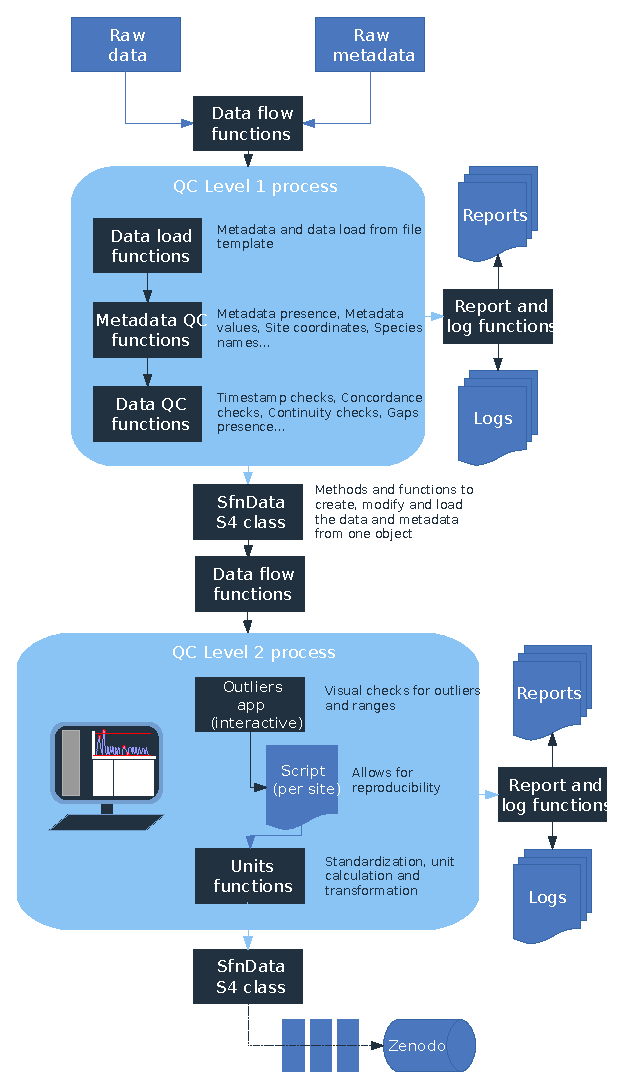
\includegraphics[width=0.7\linewidth]{figure/CH3/Figure1} 

}

\caption[Overview of the SAPFLUXNET data workflow.]{Overview of the SAPFLUXNET data workflow. Data files are received from data contributors, and undergo several quality-control processes (QC1 and QC2). Both, QC1 and QC2 produce an .RData object of the custom-designed sfn-data S4 class storing all data, metadata and data flags for each dataset. The progress and results of the QC processes are monitored through individual reports and log files. The final outcome, is stored in a folder structure with a either single .RData file for each dataset or a set of seven csv files for each dataset.}\label{fig:Ch2plot1}
\end{figure}
\subsection{Data harmonisation and quality control:
QC2}\label{data-harmonisation-and-quality-control-qc2}

Datasets entering QC2 underwent several data cleaning and data
harmonisation processes (Supplement Table S2). We first ran outlier
detection and out of range checks; these checks did not delete or modify
the data, only warned about any suspicious observation (`outlier' and
`range' warnings). The outlier detection algorithm was based on a Hampel
filter, which also estimates a replacement value for a candidate outlier
(Hampel, 1974). For the range checks, we defined minimum and maximum
allowed values for all the time series variables, based on published
values of extreme weather records and maximum transpiration rates
(Cerveny et al., 2007; Manzoni et al., 2013). The outcome of outlier and
range checks were visually inspected on the actual time series being
evaluated using an interactive R Shiny application (Supplement Fig.S3).
Following expert knowledge, visually confirmed outliers were replaced by
the values estimated by the Hampel filter. Similarly, we replaced out of
range values by NA if the variable was out of its physically allowed
range (Supplement Fig.S3). Outlier and out of range `warnings' for each
observation (e.g.~for each variable and timestep) were documented in two
data flags tables, with the same dimensions as the corresponding data
tables (Supplement Fig. S2). Likewise, those observations with confirmed
problematic values, which were removed or replaced, were also flagged;
further information can be found in the `data flags' vignettes in the
`sapfluxnetr' package Granda et al. (Granda et al., 2019)\par

Final data harmonisation processes in QC2 involved unit transformations
and the calculation of derived variables (Supplement Table S2). When
plant sapwood area was provided by data contributors, we interconverted
between sap flow rate per plant and per unit sapwood area. If leaf area
was supplied, we also calculated sap flow per unit leaf area, but note
that this transformation does not take into account the seasonal
variation in leaf area. In QC2 we estimated missing environmental
variables which could be derived from related variables in the dataset
(Appendix, Table A6). We also estimated the apparent solar time and
extraterrestrial global radiation from the provided timestamp and
geographic coordinates using the R package `solaR' (Perpiñán, 2012). All
estimated or interconverted observations were flagged as `CALCULATED' in
the `env\_flags' or `sap\_flags' table (Supplement Fig. S2).\par

\subsection{Data structure}\label{data-structure}

One of the major benefits of the SAPFLUXNET data workflow is the
encapsulation of datasets in self-contained R objects of the S4 class
with a predefined structure. These objects belong to the custom-designed
`sfn\_data' class, which display different slots to store time series of
sap flow and environmental data, their associated data flags, and all
the metadata (Supplement Fig. S2). For further information please see
the `sfn\_data classes' vignette in the `sapfluxnetr' package (Granda et
al., 2019). The code identifying each dataset was created by the
combination of a `country' code, a `site' code and, if applicable, a
`stand' code and a `treatment' code. This means that several `stands'
and/or `treatments' can be present within one `site' (Supplement Table
S3).\par

At the end of the QC process, we generated a folder structure with a
first-level storing datasets as either `sfn\_data' objects or as a set
of comma-separated (csv) text files. Within each of these formats, a
second-level folder groups datasets according to how sap flow is
normalized (per plant, sapwood or leaf area); note that the same
dataset, expressing different sap flow quantities, can be present in
more than one folder (e.g. `plant' and `sapwood'). Finally, the third
level contains the data files for each dataset: either a single
`sfn\_data' object storing all data and metadata, or all the individual
csv files. More details on the data structure can be found in the
`sapfluxnetr-quick-guide' vignette in the `sapfluxnetr' package (Granda
et al., 2019).\par

\section{The SAPFLUXNET database}\label{the-sapfluxnet-database}

\subsection{Data coverage}\label{data-coverage}

The SAPFLUXNET version 0.1.5 database harbours 202 globally distributed
datasets (Fig. 2a, Supplement Fig. S4 and Table S3), from 121
geographical locations, with Europe, Eastern USA and Australia
especially well represented. These datasets were represented in the
bioclimatic space using the terrestrial biomes delimited by Whittaker
(Fig. 2b), but note that, as any bioclimatic classification, it has its
limitations. Datasets have been compiled from all terrestrial biomes,
except for temperate rainforests, although some tropical montane sites
have been included. Woodland/shrubland and temperate forest biomes are
the most represented in the database adding up to 80\% of the datasets
(Fig. 2b). However, large forested areas in the tropics and in boreal
regions are still not well represented (Fig. 2a,b). Looking at the
distribution by vegetation type (Fig. 2c), evergreen needleleaf forest
is the most represented vegetation type (65 datasets), followed by
deciduous broadleaf forest (47 datasets) and evergreen broadleaf forest
(43 datasets).\par

SAPFLUXNET contains sap flow data for 2714 individual plants (1584
angiosperms and 1130 gymnosperms), belonging to 174 species (141
angiosperms and 33 gymnosperms), 95 different genera and 45 different
families (Supplement, Table S4-S5). All species but one, Elaeis
guineensis, a palm, are tree species. Pinus and Quercus are the most
represented genera (Fig. 3b). Amongst the gymnosperms, Pinus sylvestris,
Picea abies and Pinus taeda are the three most represented species with
data provided on 290, 178 and 107 trees, respectively (Fig. 3a). For the
angiosperms, Acer saccharum, Fagus sylvatica and Populus tremuloides are
the most represented species, with 162, 116 and 104 trees, respectively,
although most Acer saccharum data come from a single study with a very
large sample size (Fig. 3a). Some species are present in more than 10
datasets: Pinus sylvestris, Picea abies, Fagus sylvatica, Acer rubrum,
Liriodendron tulipifera and Liquidambar styraciflua (Fig. 3a, Supplement
Table S4).\par

\setlength{\abovecaptionskip}{0pt}
\begin{figure}[H]

{\centering 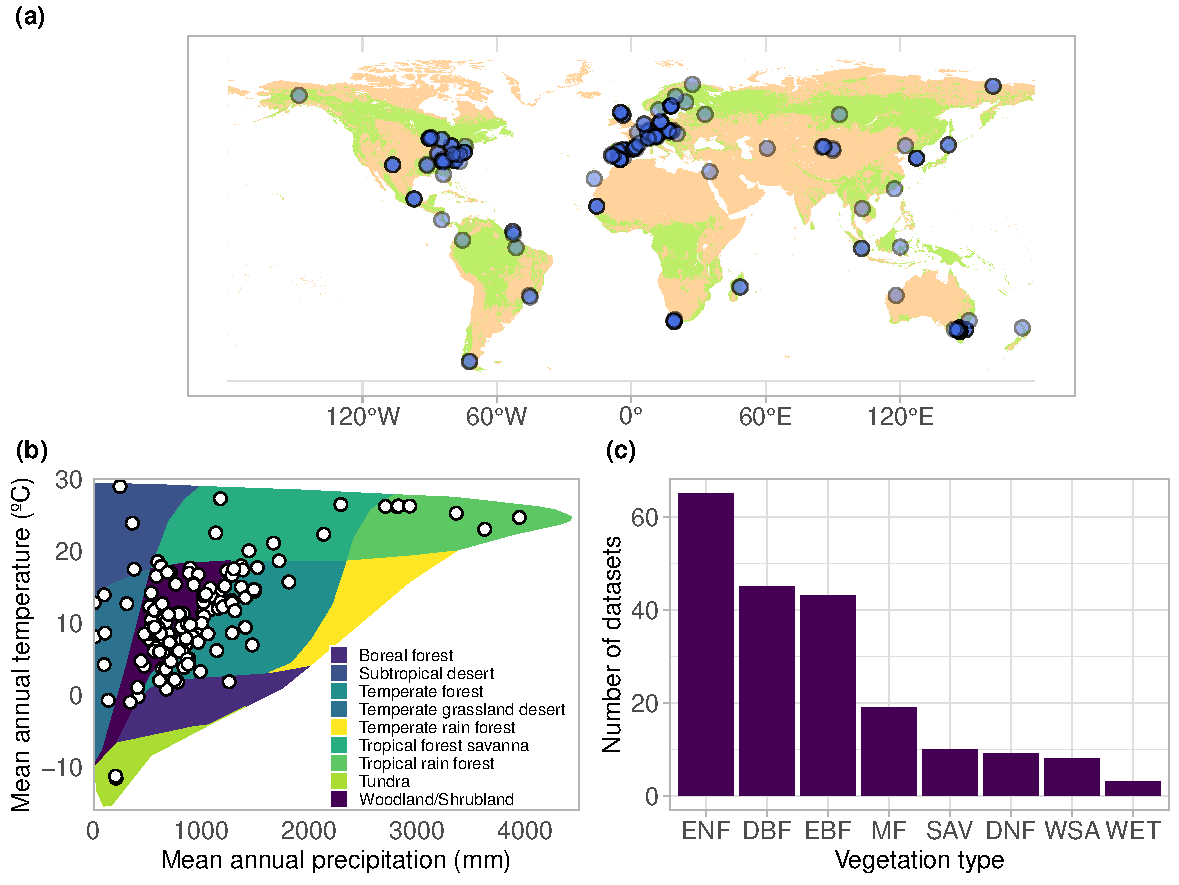
\includegraphics[width=1\linewidth]{figure/CH3/Figure2} 

}

\caption[Geographic, bioclimatic and vegetation type distribution of SAPFLUXNET datasets.]{(a) Geographic, (b) bioclimatic and (c) vegetation type distribution of SAPFLUXNET datasets. In (a) woodland area from Crowther et al. (2015) is shown in green. In (b) we represent the different datasets according to their mean annual temperature and precipitation in a Whittaker diagram showing the classification of the main terrestrial biomes. In (c) vegetation types are defined according to the International Geosphere-Biosphere Programme (IGBP) classification (ENF: Evergreen Needleleaf Forest; DBF: Deciduous Broadleaf Forest; EBF: Evergreen Broadleaf Forest; MF: Mixed Forest; DNF: Deciduous Needleleaf forest; SAV: Savannas; WSA: Woody Savannas; WET: Permanent Wetlands).}\label{fig:Ch2plot2}
\end{figure}
\setlength{\abovecaptionskip}{0pt}
\begin{figure}[H]

{\centering 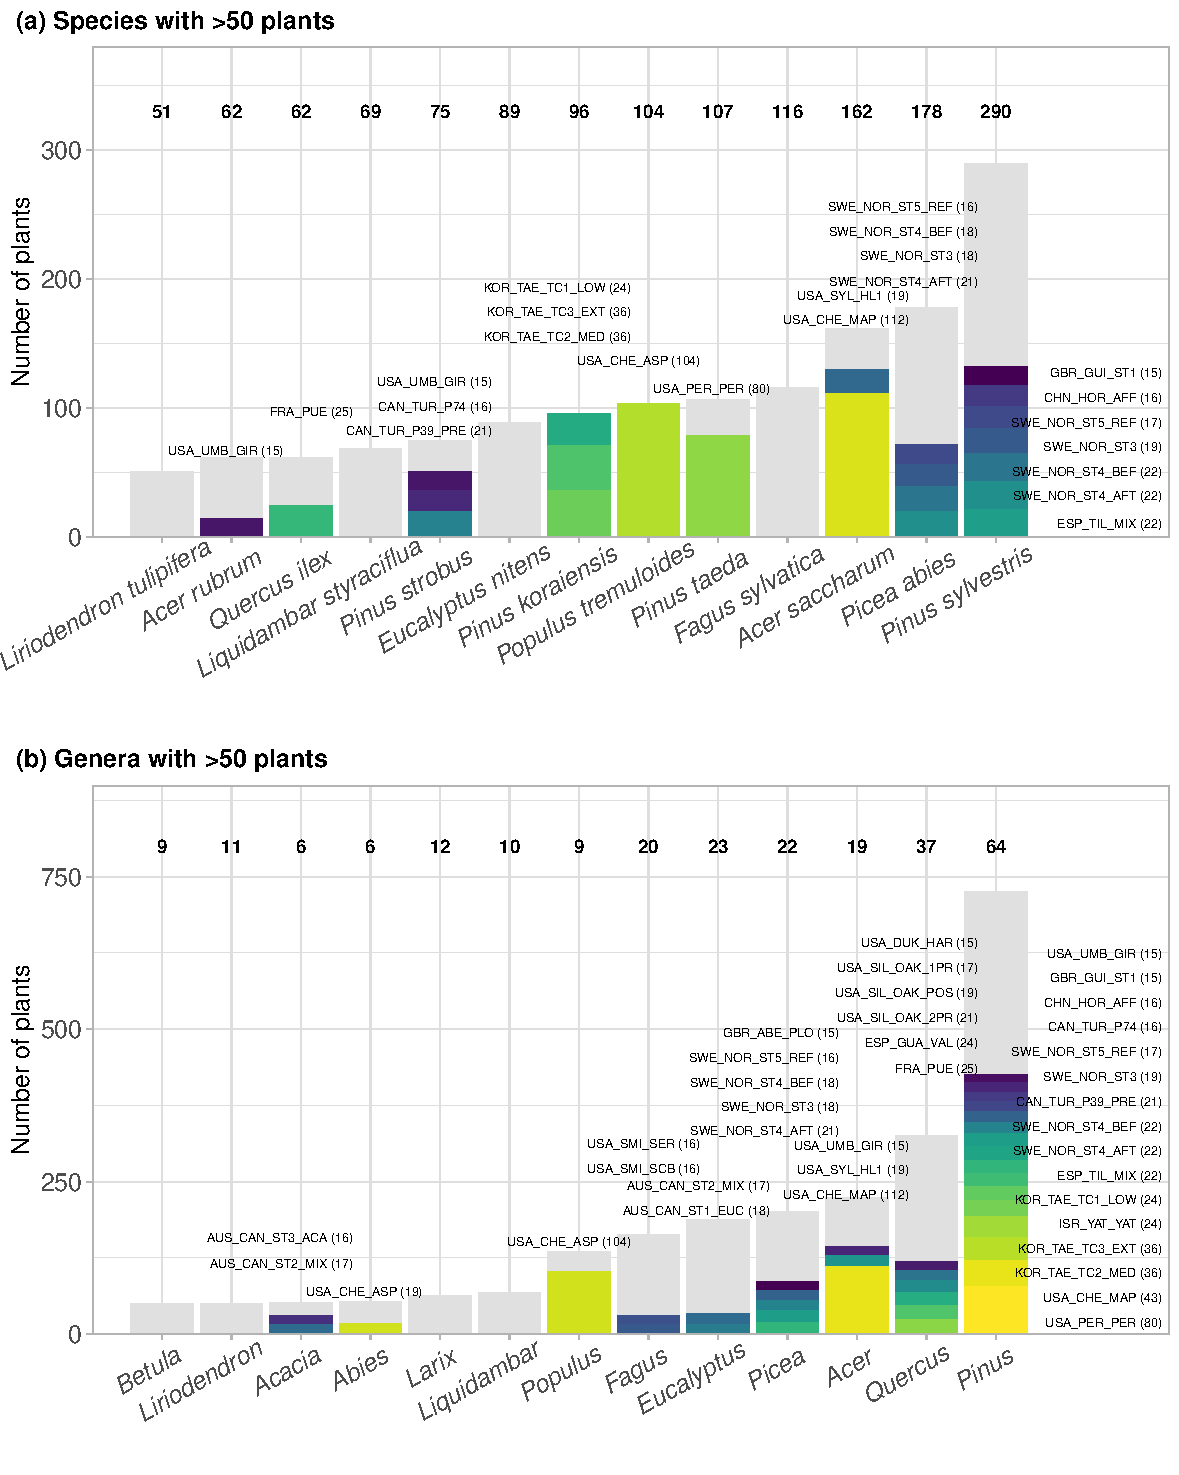
\includegraphics[width=1\linewidth]{figure/CH3/Figure3} 

}

\caption[Taxonomic distribution of genera and species in SAPFLUXNET.]{Taxonomic distribution of genera and species in SAPFLUXNET, showing (a) species and (b) genera with > 50 plants in the database. Total bar height depicts number of plants per species (a) or genera (b). Numbers on top of each bar show the number of datasets where each species (a) or genus (b) is present. Colours other than grey highlight datasets with 15 or more plants of a given species (a) or genus (b). Bar height for a given colour is proportional to the number of plants in the corresponding dataset, which is also shown in parentheses next to the dataset code.}\label{fig:Ch2plot3}
\end{figure}
\subsection{Methodological aspects}\label{methodological-aspects}

For more than 90\% of the plants, sap flow at the whole-plant level is
available (either directly provided by contributors or calculated in the
QC process); this is important for upscaling SAPFLUXNET data to the
stand level (cf.~section 4.2). Because the leaf area of the measured
plants is often not available as metadata, sap flow per unit leaf area
was estimated for only 18.6\% of the individuals (Fig. 4). The heat
dissipation method is the most frequent method in the database (HD,
66.4\% of the plants), followed by the trunk sector heat balance (TSHB,
16.4\%) and the compensation heat pulse method (CHP, 8.4\%) (Fig. 4).
This distribution is broadly similar to the use of each method
documented in the literature, although the TSHB method is
overrepresented here, compared to the current use of this method by the
sap flow community (Flo et al., 2019; Poyatos et al., 2016). Some
methods, especially those belonging to the heat pulse family and the
cyclic (or transient) heat dissipation (CHD) method are mostly used in
angiosperms, while the TSHB and the heat field deformation (HFD) methods
are more frequently used in gymnosperms (Fig. 4).\par

\setlength{\abovecaptionskip}{0pt}
\begin{figure}[hbt!]

{\centering 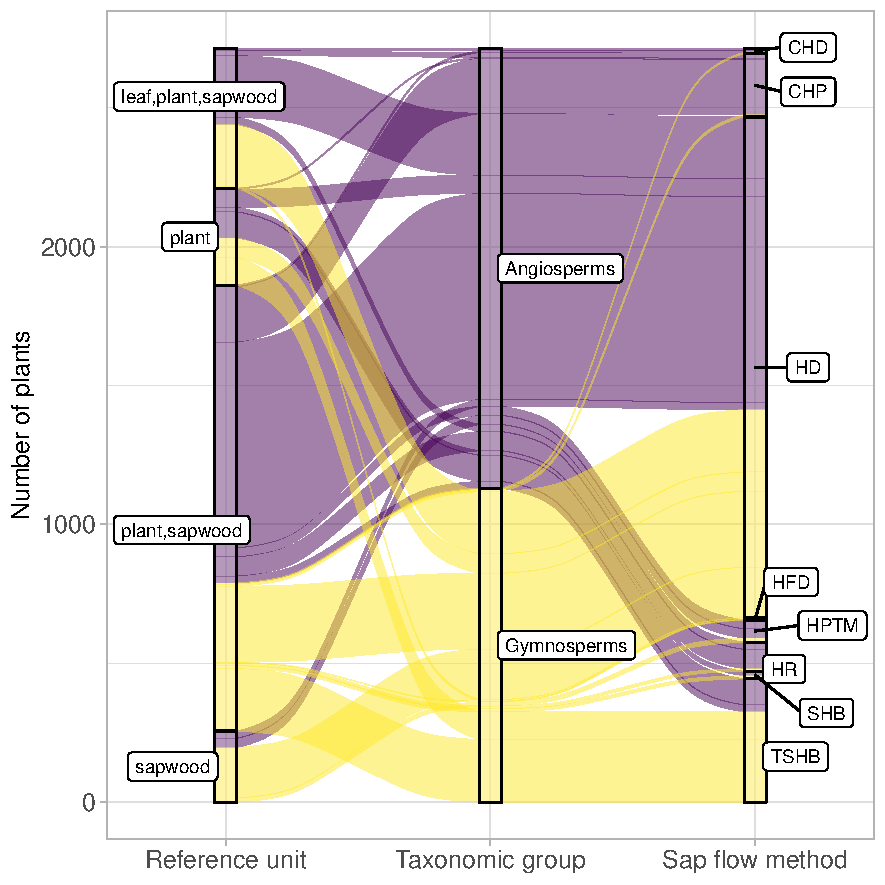
\includegraphics[width=1\linewidth]{figure/CH3/Figure4} 

}

\caption[Distribution of plants according to major taxonomic group and sap flow method.]{Distribution of plants in SAPFLUXNET according to major taxonomic group (angiosperms, gymnosperms), sap flow method (CHD:cycling heat dissipation; CHP: compensation heat pulse; HD: heat dissipation; HFD: heat field deformation: HPTM: heat pulse T-max (HPTM): HRM: heat ratio (HR); SHB: stem heat balance; TSHB: trunk sector heat balance) and reference unit for the expression of sap flow (plant, sapwood area, leaf area). Combinations of reference units imply that data are present in multiple units.}\label{fig:Ch2plot4}
\end{figure}
Calibration of sap flow sensors and scaling from point measurements to
the whole-plant can be critical steps towards accurate estimates of
absolute sap flow rates. In SAPFLUXNET, most of the sap flow time series
have not undergone a species-specific calibration, with the CHD method
showing the highest percentage of calibrated time series (Table 1). This
lack of calibrations may be relevant for the more empirical heat
dissipation methods (HD and CHD), which have been shown to consistently
underestimate sap flow rates (Flo et al., 2019; Peters et al., 2018;
Steppe et al., 2010). Radial integration of single-point sap flow
measurements is more frequent than azimuthal integration (Table 2),
except for the CHD method. A large number of plants using the HD method,
and all plants measured using the HPTM method, do not employ any radial
integration procedure. In contrast, the CHP, HR, SHB, and TSHB methods
are those which more frequently addressed radial variation in one way or
another (Table 2). Azimuthal integration procedures are also more
frequent when the TSHB method is used (Table 2).\par
\begin{table}[!h]

\caption[Number of sap flow times series in SAPFLUXNET depending on whether they were calibrated for the different sap flow methods.]{\label{tab:Ch3T1}Number of sap flow times series in SAPFLUXNET depending on whether they were calibrated (species-specific), non-calibrated or this information was not provided, for the different sap flow methods: cyclic (or transient) heat dissipation (CHD), compensation heat pulse (CHP), heat dissipation (HD), heat field deformation (HFD), heat pulse T-max (HPTM), heat ratio (HR), stem heat balance (SHB) and trunk sector heat balance (TSHB). The percentage of calibrated time series was expressed with respect to the total number of sap flow time series for each method.}
\centering
\fontsize{10}{12}\selectfont
\begin{tabular}[t]{ccccc}
\toprule
Method & Calibrated & Non-calibrated & Not provided & \% calibrated\\
\midrule
CHD & 6 & 13 & 0 & 31.6\\
CHP & 29 & 42 & 157 & 12.7\\
HD & 214 & 1491 & 98 & 11.9\\
HR & 3 & 55 & 47 & 2.9\\
TSHB & 7 & 433 & 4 & 1.6\\
HFD & 0 & 8 & 0 & 0.0\\
HPTM & 0 & 80 & 0 & 0.0\\
SHB & 0 & 27 & 0 & 0.0\\
\bottomrule
\end{tabular}
\end{table}
\begin{table}

\caption[Number of plants in the SAPFLUXNET database using different radial and azimuthal integration.]{\label{tab:Ch3T2}Number of plants in the SAPFLUXNET database using different radial and azimuthal integration approaches for the different sap flow methods: cyclic (or transient) heat dissipation (CHD), compensation heat pulse (CHP), heat dissipation (HD), heat field deformation (HFD), heat pulse T-max (HPTM), heat ratio (HR), stem heat balance (SHB) and trunk sector heat balance (TSHB).}
\centering
\resizebox{\linewidth}{!}{
\fontsize{10}{12}\selectfont
\begin{tabular}[t]{ccc>{\centering\arraybackslash}p{3.5cm}>{\centering\arraybackslash}p{2.5cm}c}
\toprule
\multicolumn{6}{l}{\textbf{Azimuthal integration}} \\
\cmidrule(l{3pt}r{3pt}){1-6}
Method & Measured & Sensor-integrated & Corrected, measured azimuthal variation & No azimuthal correction & Not provided\\
\midrule
CHD & 15 & 0 & 0 & 0 & 4\\
CHP & 61 & 0 & 0 & 167 & 0\\
HD & 216 & 0 & 520 & 1021 & 46\\
HFD & 0 & 0 & 0 & 8 & 0\\
HPTM & 0 & 0 & 0 & 80 & \vphantom{1} 0\\
HR & 7 & 0 & 2 & 88 & 8\\
SHB & 0 & 0 & 0 & 27 & 0\\
TSHB & 0 & 25 & 191 & 219 & 9\\
\addlinespace[0.5em]
\hline
\multicolumn{6}{l}{\textbf{Radial integration}}\\
\hline
\hspace{1em}Method & Measured & Sensor-integrated & Corrected, measured radial variation & No radial correction & Not provided\\
\hline
\hspace{1em}CHD & 0 & 0 & 6 & 13 & 0\\
\hspace{1em}CHP & 222 & 0 & 6 & 0 & 0\\
\hspace{1em}HD & 77 & 3 & 645 & 703 & 142\\
\hspace{1em}HFD & 2 & 0 & 0 & 6 & 0\\
\hspace{1em}HPTM & 0 & 0 & 0 & 80 & 0\\
\hspace{1em}HR & 57 & 1 & 42 & 3 & 2\\
\hspace{1em}SHB & 0 & 27 & 0 & 0 & 0\\
\hspace{1em}TSHB & 0 & 338 & 8 & 89 & 9\\
\bottomrule
\end{tabular}}
\end{table}
\subsection{Plant characteristics}\label{plant-characteristics}

Plant-level metadata is almost complete (99.5\% of the individuals) for
diameter at breast height (DBH), while sapwood area and sapwood depth,
important variables for sap flow upscaling, are not available, or could
not be estimated, for 23\% and 47\% of the plants, respectively. Plant
height and plant age are missing for 42\% and 62\% of the individuals,
respectively. Sap flow data in SAPFLUXNET are representative of a broad
range of plant sizes (Fig. 5a). The distribution of DBH showed a median
of 25.0 cm and 20.4 cm for gymnosperms and angiosperms, respectively,
with a long tail towards the largest plants, two Mortoniodendron
anisophyllum trees from a tropical forest in Costa Rica that measured
\textgreater{} 200 cm (Fig. 5a). The largest gymnosperm tree in
SAPFLUXNET (176 cm in DBH) is a kauri tree (Agathis australis) from New
Zealand. The distribution of plant heights is less skewed, with similar
medians for angiosperms (17.6 m) and gymnosperms (17.5 m). The tallest
plants are located in a tropical forest in Indonesia, where a Pouteria
firma tree reached 44.7 m. Remarkably, of the 16 plants taller than 40
m, over 60\% are Eucalyptus species. The tallest gymnosperm (36.2 m) is
a Pinus strobus from NE USA.\par

\setlength{\abovecaptionskip}{0pt}
\begin{figure}[hbt!]

{\centering 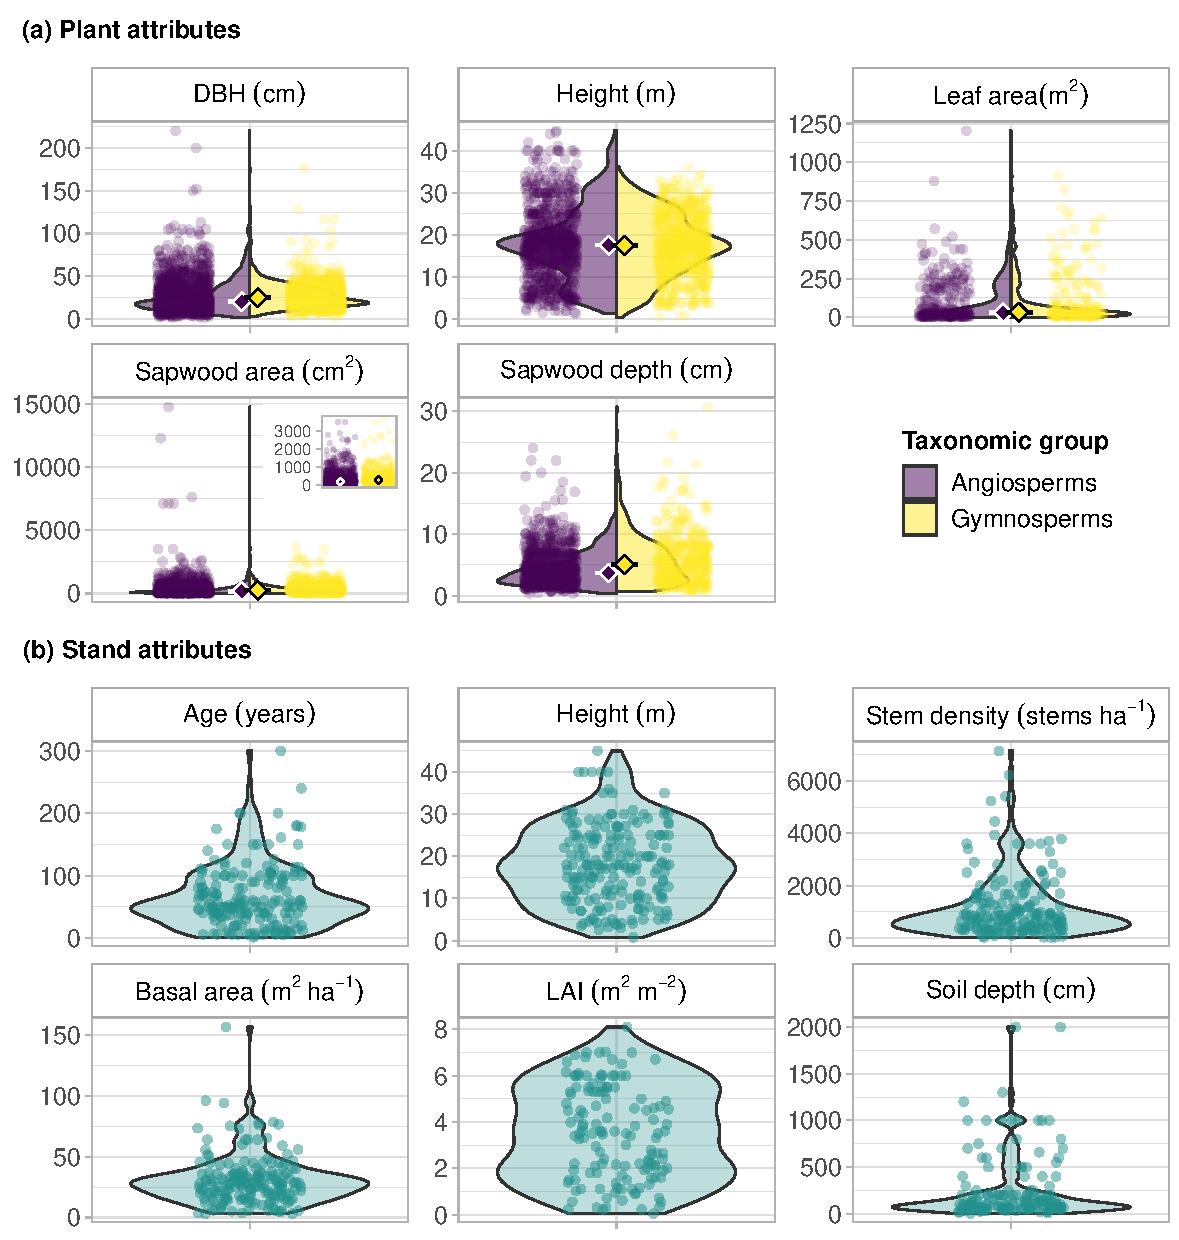
\includegraphics[width=1\linewidth]{figure/CH3/Figure5} 

}

\caption[Characteristics of trees and stands in the SAPFLUXNET database.]{Characteristics of trees and stands in the SAPFLUXNET database. Panel (a) shows plant data and kernel density plots of the main plant attributes, coloured by taxonomic group (angiosperms and gymnosperms): diameter at breast height (DBH), plant height, sapwood area, sapwood depth and leaf area. The inset in the sapwood area panel zooms in values lower than 5000 cm². Panel (b) shows stand data and kernel density plots of the main stand attributes: stand age, stand height, stem density, stand basal area,leaf area index (LAI) and soil depth.}\label{fig:Ch2plot5}
\end{figure}
Plant size metadata in SAPFLUXNET is complemented with plant-level data
of sapwood and leaf area, that provide information on the functional
areas for water transport and loss (Fig. 5a). Distributions of sapwood
and leaf area show highly skewed distributions, with long tails towards
the largest values and slightly higher median values for gymnosperms
(262 cm2 and 33.0 m2 for sapwood and leaf areas, respectively), compared
to angiosperms (168 cm2 and 29.9 m2). Accordingly, median sapwood depth
is also higher for gymnosperms (5.1 cm) compared to angiosperms (3.7
cm). The largest trees (Mortoniodendron, Pouteria, Agathis) with deep
sapwood (17--24 cm) are also those with largest sapwood areas. Many
large angiosperm trees from tropical (CRI\_TAM\_TOW, IDN\_PON\_STE,
GUF\_GUY\_ST2; see Table S3 for dataset codes) and temperate forests
(Fagus grandifolia, USA\_SMIC\_SCB) also show large sapwood areas
(\textgreater{} 5000 cm2), but the plant with the deepest sapwood is a
gymnosperm, an Abies pinsapo in Spain with 30.7 cm of sapwood depth.\par

\subsection{Stand characteristics}\label{stand-characteristics}

Stand-level metadata include several variables associated with
management, vegetation structure and soil properties. Half of the
datasets originate from naturally regenerated, unmanaged stands, and
13.9\% come from naturally regenerated but managed stands. Plantations
add up to 32.2\% and orchards only represent 4\% of the datasets.
Reporting of structural variables is mixed, with stand height, age,
density and basal area showing relatively low missingness (6.4\%,
11.4\%, 12.9\% and 13.4\%, respectively); in contrast, soil depth and
LAI are missing from 26.7\% and 33.7\% of the datasets.\par

SAPFLUXNET datasets originate from stands with diverse structural
characteristics. Median stand age is 54 years and there are several
datasets coming from \textgreater{}100 year-old forests (Fig. 5b). Stand
height shows a similar range and distribution of values compared to
individual plant height (Fig. 5a,b). The denser stands correspond to
coppiced evergreen oak stands from Mediterranean forests (FRA\_PUE,
ESP\_TIL\_OAK), species-rich tropical forests (MDG\_SEM\_TAL) or
relatively young temperate forests (e.g.~FRA\_HES\_HE1\_NON,
USA\_CHE\_MAP). The sparsest stands (\textless{} 200 stems ha-1)
correspond to tree-grass savanna systems (Spain, Portugal, Australia,
Senegal), dry woodlands (China), or oil palm plantations in Indonesia
(IDN\_JAM\_OIL). Stands with the largest basal areas (\textgreater{} 70
m2 ha-1) are mostly dominated by broadleaf species, except for a Picea
abies plantation in Sweden (SWE\_SKO\_MIN).\par

The distribution of leaf area index (LAI) shows a median of 3.5 m2 m-2,
with the largest values observed in temperate (CZE\_BIK, USA\_DUK\_HAR,
HUN\_SIK) and tropical (GUF\_GUY\_GUY, COL\_MAC\_SAF\_RAD) forests. The
stands with the lowest LAI correspond to the sparse woodlands from
Mediterranean and semi-arid locations and also those from forests near
altitudinal or latitudinal tree-lines (FIN\_PET, AUT\_TSC). SAPFLUXNET
datasets show a median soil depth of 100 cm, with only a dozen datasets
originated from sites with soils deeper than 10 m (Fig. 5b).\par

The number of plants per dataset is highly variable, with most of the
datasets (86\%) containing data for at least 4 trees and 46\% of the
datasets having data for at least 10 trees (Fig. 6a, see also Fig. 9).
\par

\setlength{\abovecaptionskip}{0pt}
\begin{figure}[hbt!]

{\centering 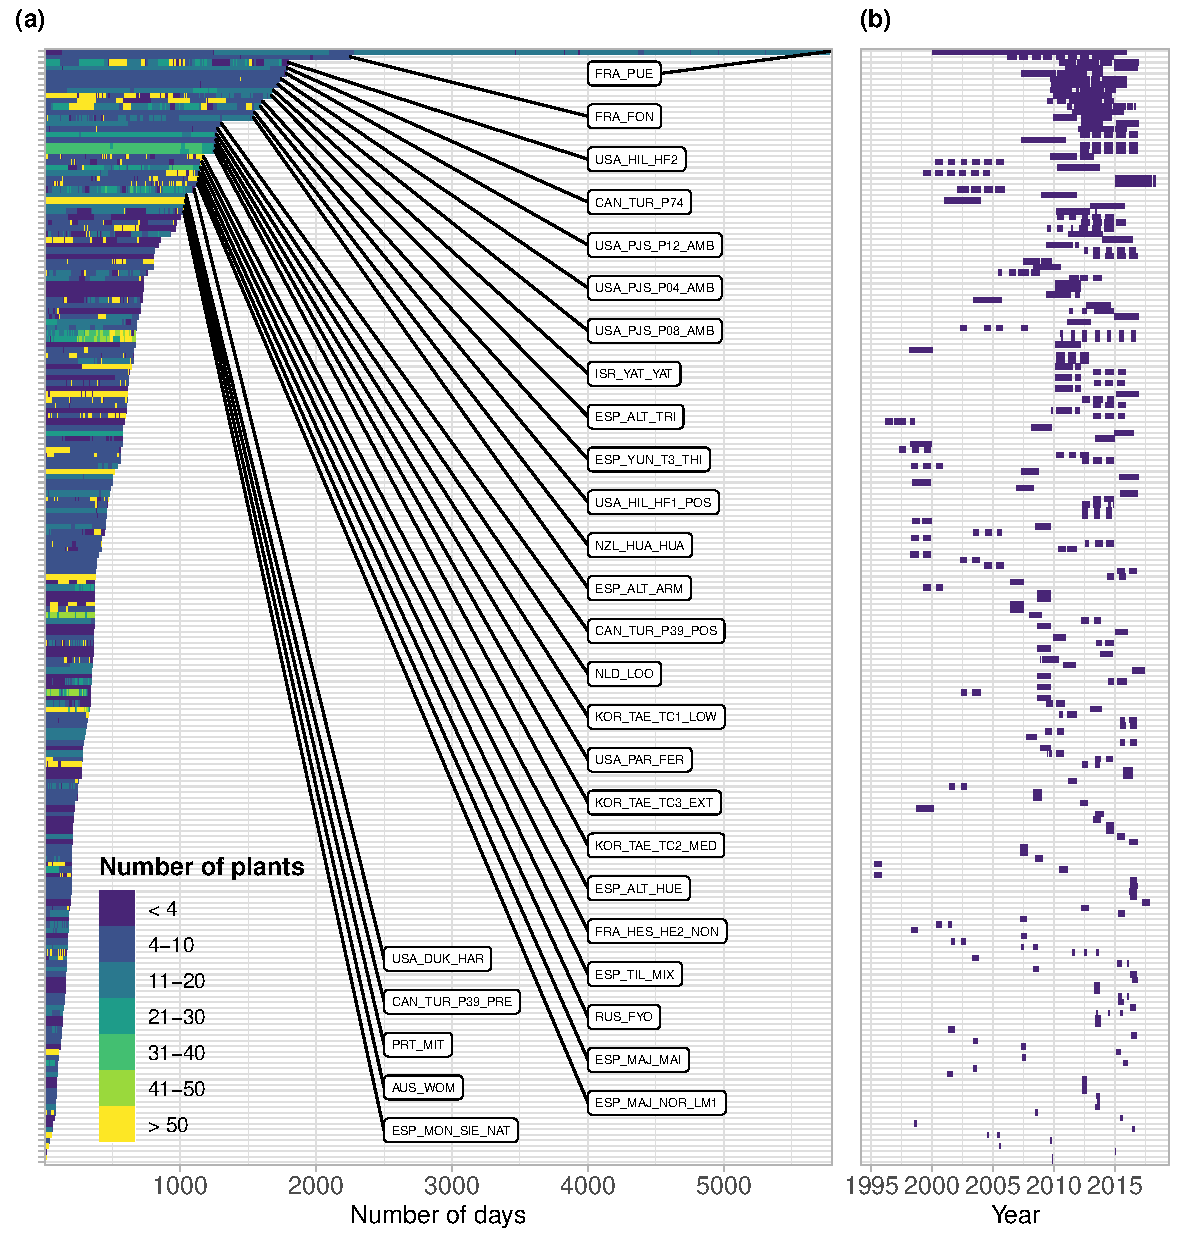
\includegraphics[width=1\linewidth]{figure/CH3/Figure6} 

}

\caption[Duration and number of plants mesured in each dataset.]{(a) Measurement duration of SAPFLUXNET datasets expressed in number of days with sap flow data and coloured by the number of plants measured on each day . The 30 longest datasets are labelled. For each dataset in panel (a), panel (b) shows its corresponding measurement period.}\label{fig:Ch2plot6}
\end{figure}
\subsection{Temporal characteristics}\label{temporal-characteristics}

The oldest datasets in SAPFLUXNET go back to 1995 (GBR\_DEV\_CON,
GBR\_DEV\_DRO) while the most recent data reach up to 2018 (datasets
from the ESP\_MAJ cluster of sites). Several multi-year datasets are
present in SAPFLUXNET (Fig. 6), with 50\% of the datasets spanning a
period of at least 3 years, and some datasets being extraordinarily long
(16 years in FRA\_PUE). Frequently, the datasets only cover the `growing
season' periods, or even shorter periods for some sites which were
eventually included because they improved the ecological and geographic
coverage of the database (e.g.~ARG\_MAZ, ARG\_TRE as representative of
deciduous Nothofagus forest in South Patagonia). In contrast, a few
datasets show continuous records over multiple years (Fig. 6b). Amongst
the longest datasets, most of them come from European or North American
sites (Fig. 6), except some datasets from Israel (ISR\_YAT\_YAT, 7
years), Russia (RUS\_FYO, 7 years), South Korea (KOR\_TAE cluster of
sites, 6 years) or New Zealand (NZL\_HUA\_HUA, 5 years).\par 

SAPFLUXNET provides an unprecedented database to study the detailed
temporal dynamics of plant transpiration across species and sites
globally. Sub-daily records of sap flow (e.g.~at least at hourly
timesteps) are available for extended periods (Fig. 6b), allowing to
address both seasonal and diel patterns in water use regulation by trees
and how these temporal patterns change across species or years across
terrestrial biomes, reflecting different phenologies and water-use
strategies. For instance, in Mediterranean forests, evergreen species
such as Quercus ilex, Arbutus unedo and Pinus halepensis show moderate
sap flow the whole year round, while the deciduous Quercus pubescens
shows higher sap flow density during a shorter period and its water use
is heavily reduced during a dry year (2012) (Fig. 7a). Temperate forests
without water availability limitations show relatively high flows during
the growing season and similar diel sap flow patterns among species
(Fig. 7b). In contrast, tropical forests show moderate to high sap flow
rates during the entire year, with different dynamics in the intradaily
water use regulation across species. For example, Inga sp. in a highly
diverse wet tropical forest in Costa Rica, reduced sap flow during
mid-day hours compared to co-existing species (Fig. 7c).\par

\setlength{\abovecaptionskip}{0pt}
\begin{figure}[hbt!]

{\centering 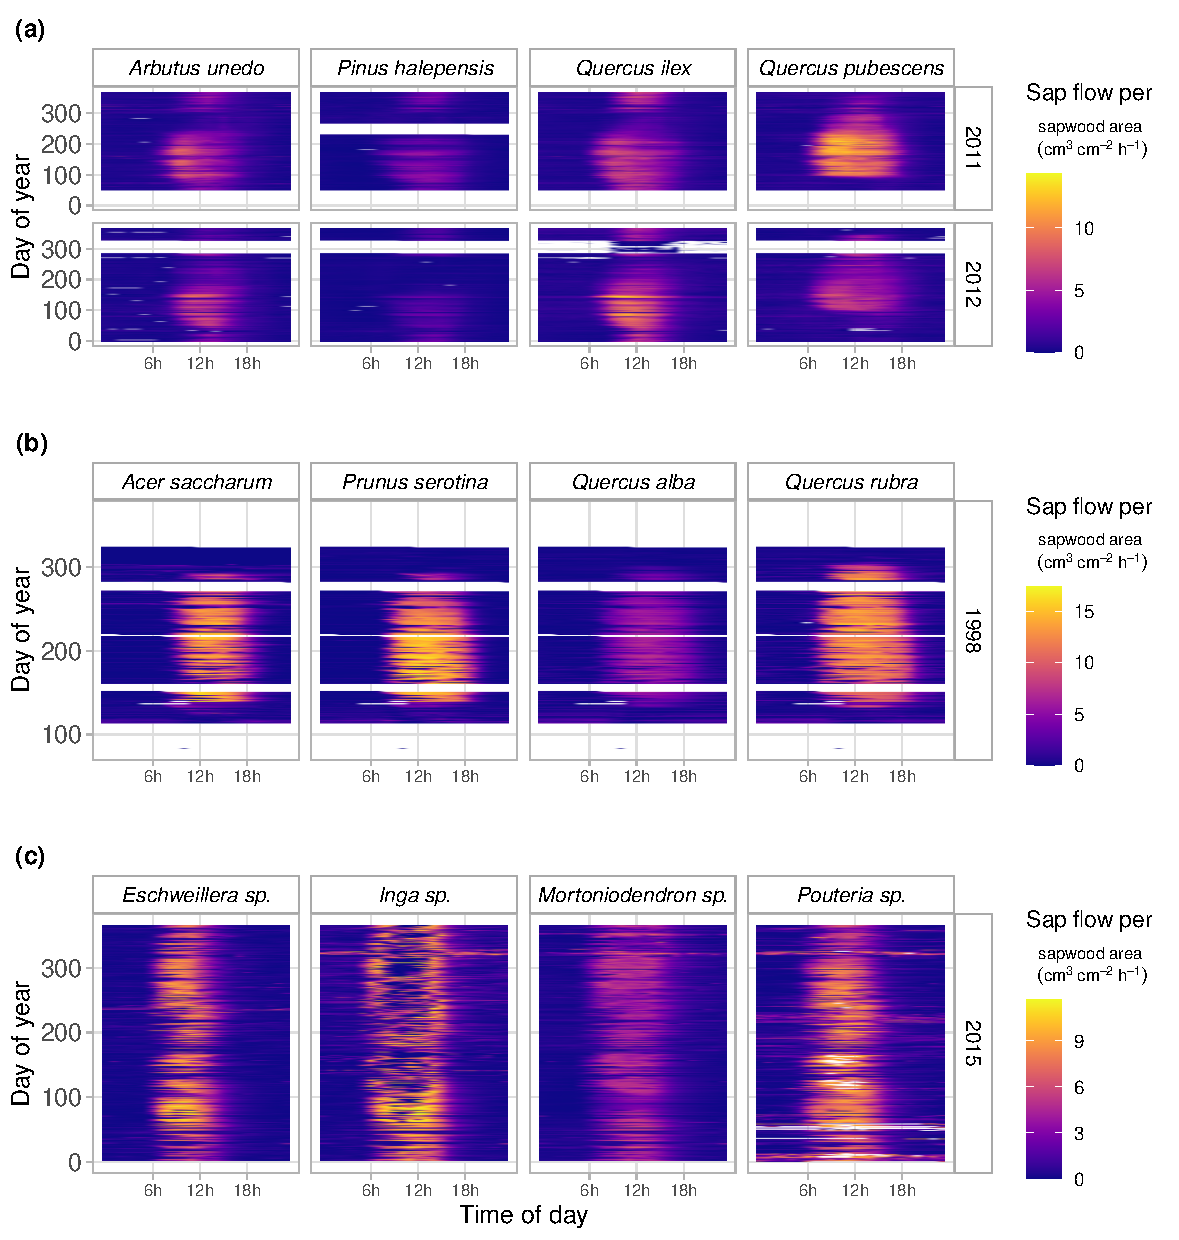
\includegraphics[width=1\linewidth]{figure/CH3/Figure7} 

}

\caption[Fingerprint plots showing hourly sap flow per unit sapwood area.]{Fingerprint plots showing hourly sap flow per unit sapwood area (colour scale) as a function of hour of day (x-axis) and day of year (y-axis) for a selection of SAPFLUXNET sites with at least four co-occurring species. Panel (a) shows data from a Woodland/Shrubland forest in NE Spain (ESP\_CAN), for an average (2011) and a dry (2012) year. Panel (b) shows data for a mesic Temperate forest (USA\_WVF) and panel (c) shows data for a Tropical forest (CRI\_TAM\_TOW). For this latter site, only 4 of the 17 measured species are shown and some of them were only identified at the genus level.}\label{fig:Ch2plot7}
\end{figure}
\subsection{Availability of environmental
data}\label{availability-of-environmental-data}

All SAPFLUXNET datasets contain ancillary time series of the main
hydrometeorological drivers of transpiration, accompanied by information
on where these variables had been measured (Fig. 8a). Air temperature is
available for all datasets. Although vapour pressure deficit (VPD) was
originally absent in 38\% of the datasets (Fig. 8a,b), we could estimate
it for those sites providing air temperature and relative humidity data
(QC Level 2, see section 2.3), and finally only 2 out of the 202
datasets have missing VPD information. For radiation variables,
shortwave radiation was most often provided, compared to
photosynthetically active and net radiation; only 8 out of 202 datasets
do not have any accompanying radiation data. Most of these environmental
variables were measured on-site, with precipitation being the variable
most frequently retrieved from nearby meteorological stations (48\% of
the datasets) (Fig. 8a). Soil water content measured at shallow depth,
typically between 0 and 30 cm below the soil surface, is provided for
56\% of the datasets, while soil moisture from deep soil layers is
available for only 27\% of the datasets.\par

\setlength{\abovecaptionskip}{0pt}
\begin{figure}[hbt!]

{\centering 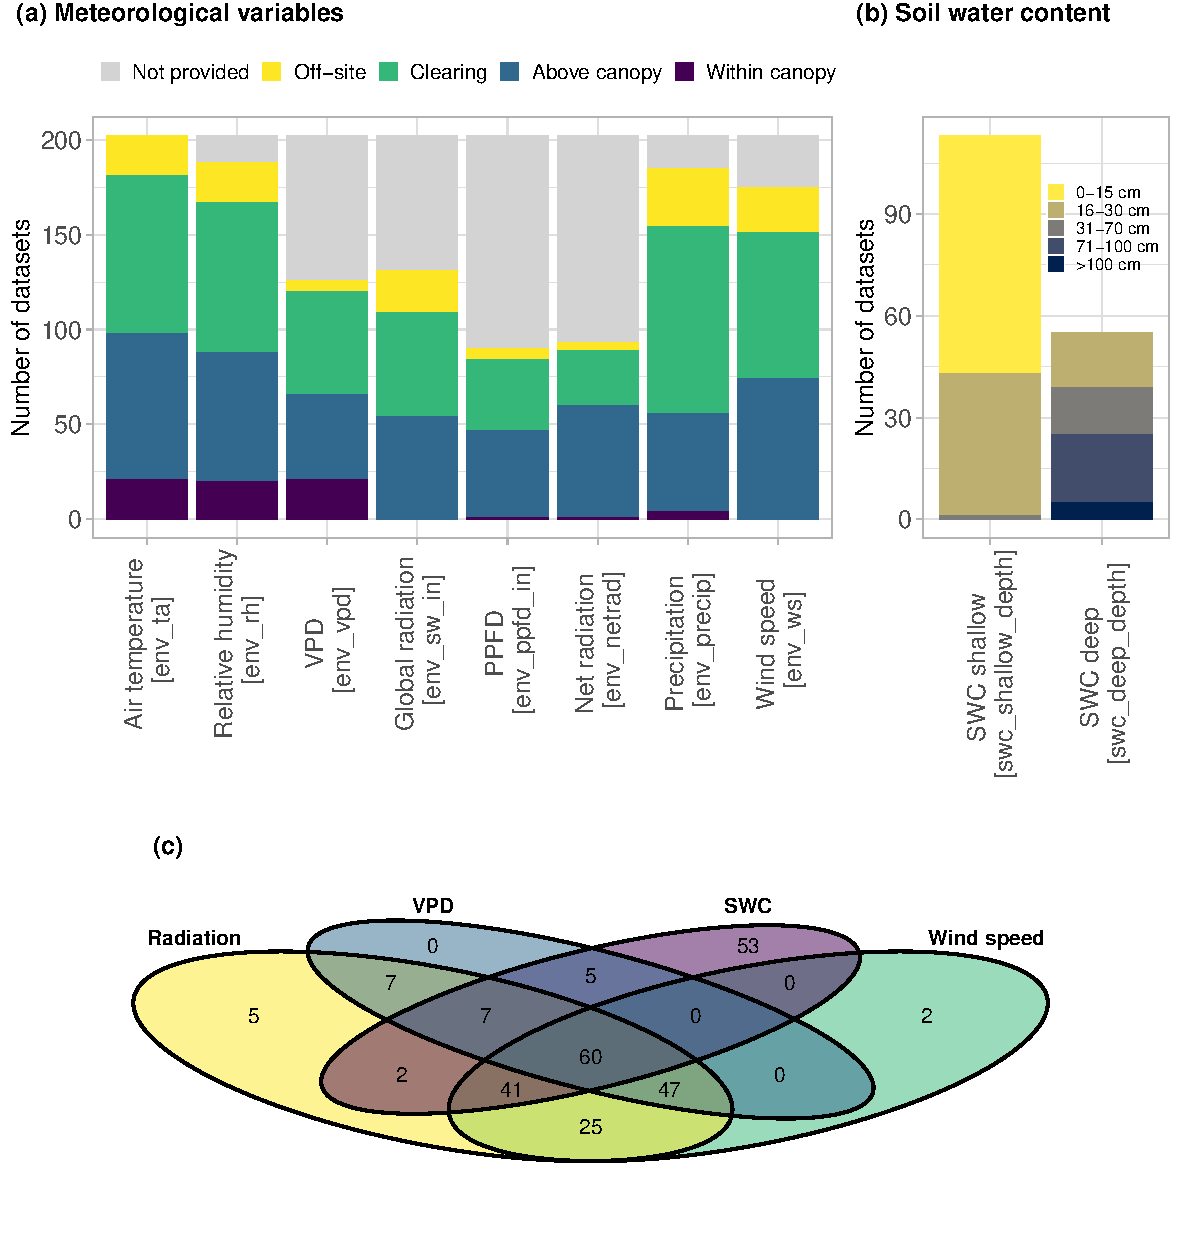
\includegraphics[width=1\linewidth]{figure/CH3/Figure8} 

}

\caption[Summary of the availability of different environmental variables in SAPFLUXNET datasets.]{Summary of the availability of different environmental variables in SAPFLUXNET datasets. (a) Distribution of meteorological variables according to sensor location (in brackets, names of the variables in the database), (b) Distribution of soil moisture variables according to the measurement depth (in brackets, names of the variables in the database). (c) Venn diagram showing the number of datasets where each combination of different environmental variables are present, grouping shortwave, PPFD and net radiation under ‘Radiation’ variables.}\label{fig:Ch2plot8}
\end{figure}
\section{Potential applications}\label{potential-applications}

\subsection{Applications in plant ecophysiology and functional
ecology}\label{applications-in-plant-ecophysiology-and-functional-ecology}

There are multiple potential applications of the SAPFLUXNET database to
assess whole-plant water use rates and their environmental sensitivity,
both across species (e.g.~Oren et al., 1999b) and at the intraspecific
level (Poyatos et al., 2007). SAPFLUXNET will allow disentangling the
roles of evaporative demand and soil water content in controlling
transpiration at the plant level, complementing recent studies looking
at how water supply and demand affect evapotranspiration at the
ecosystem level (Anderegg et al., 2018; Novick et al., 2016). The
availability of global sap flow data at sub-daily time resolution and
spanning entire growing seasons will allow focusing on how maximum water
use and its environmental sensitivity varies with plant-level attributes
such as stem diameter (Dierick and Hölscher, 2009; Meinzer et al.,
2005), tree height (Novick et al., 2009; Schäfer et al., 2000),
hydraulic (Manzoni et al., 2013; Poyatos et al., 2007) and other plant
traits (Grossiord et al., 2019; Kallarackal et al., 2013). SAPFLUXNET
thus provides an unprecedented tool to understand how structural and
physiological traits scale-up to whole-plant regulation of water fluxes
(McCulloh et al., 2019), and how this integration determines drought
responses (Choat et al., 2018) and post-drought recovery patterns (Yin
and Bauerle, 2017). Analyses of the temporal dynamics of plant water use
in response to specific drought events, as recently assessed for gross
primary productivity (e.g.~Schwalm et al., 2017), can also help to
quantify drought legacy effects, including the reversibility of
drought-induced losses of hydraulic conductivity at the plant level.\par

SAPFLUXNET will allow new insights into within-day patterns and controls
in whole-plant water use, which can disclose the fine details of its
physiological regulation. Circadian rhythms can modulate stomatal
responses to the environment, potentially affecting sap flow dynamics
(e.g.~de Dios et al., 2015). Hysteresis in diel sap flow relationships
with evaporative demand and time-lags between evaporative demand and sap
flow, are two linked phenomena likely arising from plant capacitance and
other mechanisms (O'Brien et al., 2004; Schulze et al., 1985), that also
influence diel evapotranspiration dynamics (Matheny et al., 2014; Zhang
et al., 2014). A major driver of time-lags is the use of stored water to
meet the transpiration demand (Phillips et al., 2009), which can now be
analysed across species, plant sizes or drought conditions using time
series analyses, simplified electric analogies (Phillips et al., 1997,
2004; Ward et al., 2013) or detailed water transport models (Bohrer et
al., 2005; Mirfenderesgi et al., 2016). Night-time water use can be
substantial for some species (Forster, 2014; Resco de Dios et al.,
2019). However, available syntheses rely on study-specific
quantification of what constitutes nocturnal sap flow and do not address
possible methodological influences (Zeppel et al., 2014). SAPFLUXNET
will allow applying a consistent estimation of nocturnal sap flow and
control for datasets that are less suitable for the quantification of
night-time fluxes, as information on zero-flow determination is included
in the metadata (`pl\_sens\_cor\_zero', Appendix Table A5).\par

Sap flow data have been widely employed to assess changes in tree water
use after biotic (e.g.~Hultine et al., 2010) or abiotic (Oren et al.,
1999a) disturbances. Likewise, sap flow data have been used to report
changes in species and stand water use following experimental treatments
involving resource availability modifications (e.g.~Ewers et al., 1999)
or density changes (i.e.~thinning, Simonin et al., 2007). The SAPFLUXNET
database includes datasets with experimental manipulations, applied
either at the stand or at the individual level (Table 3). The main
treatments present are related to thinning, water availability changes
(irrigation, throughfall exclusion) and wildfire impact (Table 3),
potentially facilitating new data syntheses and meta-analyses using
these datasets (e.g.~Grossiord et al., 2017).\par
\begin{table}[!h]

\caption[Number of datasets, plants and species by stand-level treatment in the SAPFLUXNET database.]{\label{tab:Ch3T3}Number of datasets, plants and species by stand-level treatment in the SAPFLUXNET database.}
\centering
\fontsize{10}{12}\selectfont
\begin{tabular}[t]{cccc}
\toprule
Treatment & N sites & N plants & N species\\
\midrule
None/control & 155 & 2198 & 170\\
Thinning & 18 & 332 & 18\\
Irrigation & 9 & 36 & 4\\
Post-fire & 6 & 18 & 4\\
CO2 fertilisation & 3 & 28 & 2\\
Drought & 3 & 9 & 2\\
Soil fertilisation & 2 & 16 & 2\\
Post-mortality & 1 & 22 & 5\\
Soil fertilisation and pruning & 1 & 12 & 1\\
Soil fertilisation and thinning & 1 & 12 & 1\\
Pruning and thinning & 1 & 11 & 1\\
Soil fertilisation, pruning and thinning & 1 & 11 & 1\\
Pruning & 1 & 9 & 1\\
\bottomrule
\end{tabular}
\end{table}
The combination of SAPFLUXNET with other ecophysiological databases can
inform on the relative sensitivity of different physiological processes
in response to drought, for example those related to growth and carbon
assimilation (Steppe et al., 2015) . Within-day fluctuations of stem
diameter can be jointly analysed with co-located sap flow measurements
to study the dynamics of stored water use under drought and its
contribution to transpiration (e.g.~Brinkmann et al., 2016), and to
infer parameters on tree hydraulic functioning using mechanistic models
of tree hydrodynamics (Salomón et al., 2017; Steppe et al., 2006;
Zweifel et al., 2007). These analyses could be carried out for a large
number of species by combining SAPFLUXNET with data from the
Dendroglobal database
(\url{http://78.90.202.92/streess/databases/dendroglobal}); there are at
least 18 SAPFLUXNET datasets with dendrometer data in Dendroglobal. This
database and the International Tree-Ring Data Bank (Zhao et al., 2018)
could also be used with SAPFLUXNET to investigate, at the species level,
the link between radial growth and water use, including their
environmental sensitivity (Morán-López et al., 2014), and how these two
processes comparatively respond to drought (Sánchez-Costa et al., 2015).
Moreover, given the tight link between water use and carbon
assimilation, combining SAPFLUXNET with water-use efficiency from plant
\textbackslash{}delta13C data could potentially be used to estimate
whole-plant carbon assimilation (Hu et al., 2010; Klein et al., 2016;
Rascher et al., 2010; Vernay et al., 2020), a quantity that is difficult
to measure directly, especially in field-grown, mature trees.\par

The two first PCA axes explained 60\% of the variability of the 12
climatic variables (Appendix B Figure B.2). The niche of \emph{P.
halepensis} characterized with inter-annual variability (inter-annual
variability-based niche) was 42\% larger than the niche estimated with
the average dataset (average-based niche). These differences implied
that during the extreme climatic year, 93.3\% of unaffected forests and
63.3\% of highly affected forests were inside the \emph{P. halepensis}
niche estimated with inter-annual variability. These values diminished
to 52.8\% for unaffected forests and 21.2\% for highly affected ones
when niche was calculated with average climate (Figure 3.2).\par

\subsection{Applications in ecosystem ecology and
ecohydrology}\label{applications-in-ecosystem-ecology-and-ecohydrology}

SAPFLUXNET will provide a global look at plant water flows to bridge the
scales between plant traits and ecosystem fluxes and properties
(Reichstein et al., 2014). Vegetation structure, species composition and
differential water use strategies among and within species scale-up to
different seasonal patterns of ecosystem transpiration, with a strong
influence on ecosystem evapotranspiration and its partitioning. Global
controls on evaporative fluxes from vegetation have been mostly
addressed using ecosystem (Williams et al., 2012) or catchment
evapotranspiration data (Peel et al., 2010). These studies have
described global patterns in evapotranspiration driven by different
plant functional types or climates, but they cannot be used to quantify
and to explain the enormous variation in the regulation of transpiration
across and within taxa.\par

The SAPFLUXNET database will provide a long-demanded data source to be
used in ecohydrological research (Asbjornsen et al., 2011). Upscaling
individual measurements to the stand level (Čermák et al., 2004; Granier
et al., 1996; Köstner et al., 1998) is necessary to quantitatively
compare sap-flow based transpiration with evapotranspiration and
transpiration estimates at the ecosystem scale and beyond. Even though
SAPFLUXNET was designed to accommodate sap flow data at the plant level,
scaling to the ecosystem level is possible for many datasets. For a
basic upscaling exercise using SAPFLUXNET data (Poyatos et al., 2020b),
whole-plant sap flow can be normalised by individual basal area (as DBH
is usually available in the metadata, cf.~section 3.3), averaged for a
given species and then scaled to stand level transpiration using total
stand basal area and the fraction of basal area occupied by each
measured species (see stand metadata, Table A3). For many datasets, sap
flow data are available for the species comprising most of the stand
basal area (often even 100\%, Fig. 9), but species-based upscaling may
be unfeasible in many tropical sites (Fig. 9b), where size-based scaling
could be applied instead (e.g.~da Costa et al., 2018). Further
refinements of the upscaling procedure could be achieved by using trunk
diameter distributions of the sap flow plots (Berry et al., 2018). This
information, however, is not readily available in SAPFLUXNET, and other
data sources (e.g.~forest inventories, LIDAR data) or additional
simplifying assumptions (i.e.~applying the size distribution of measured
individuals in the dataset) would be needed.\par

\setlength{\abovecaptionskip}{0pt}
\begin{figure}[H]

{\centering 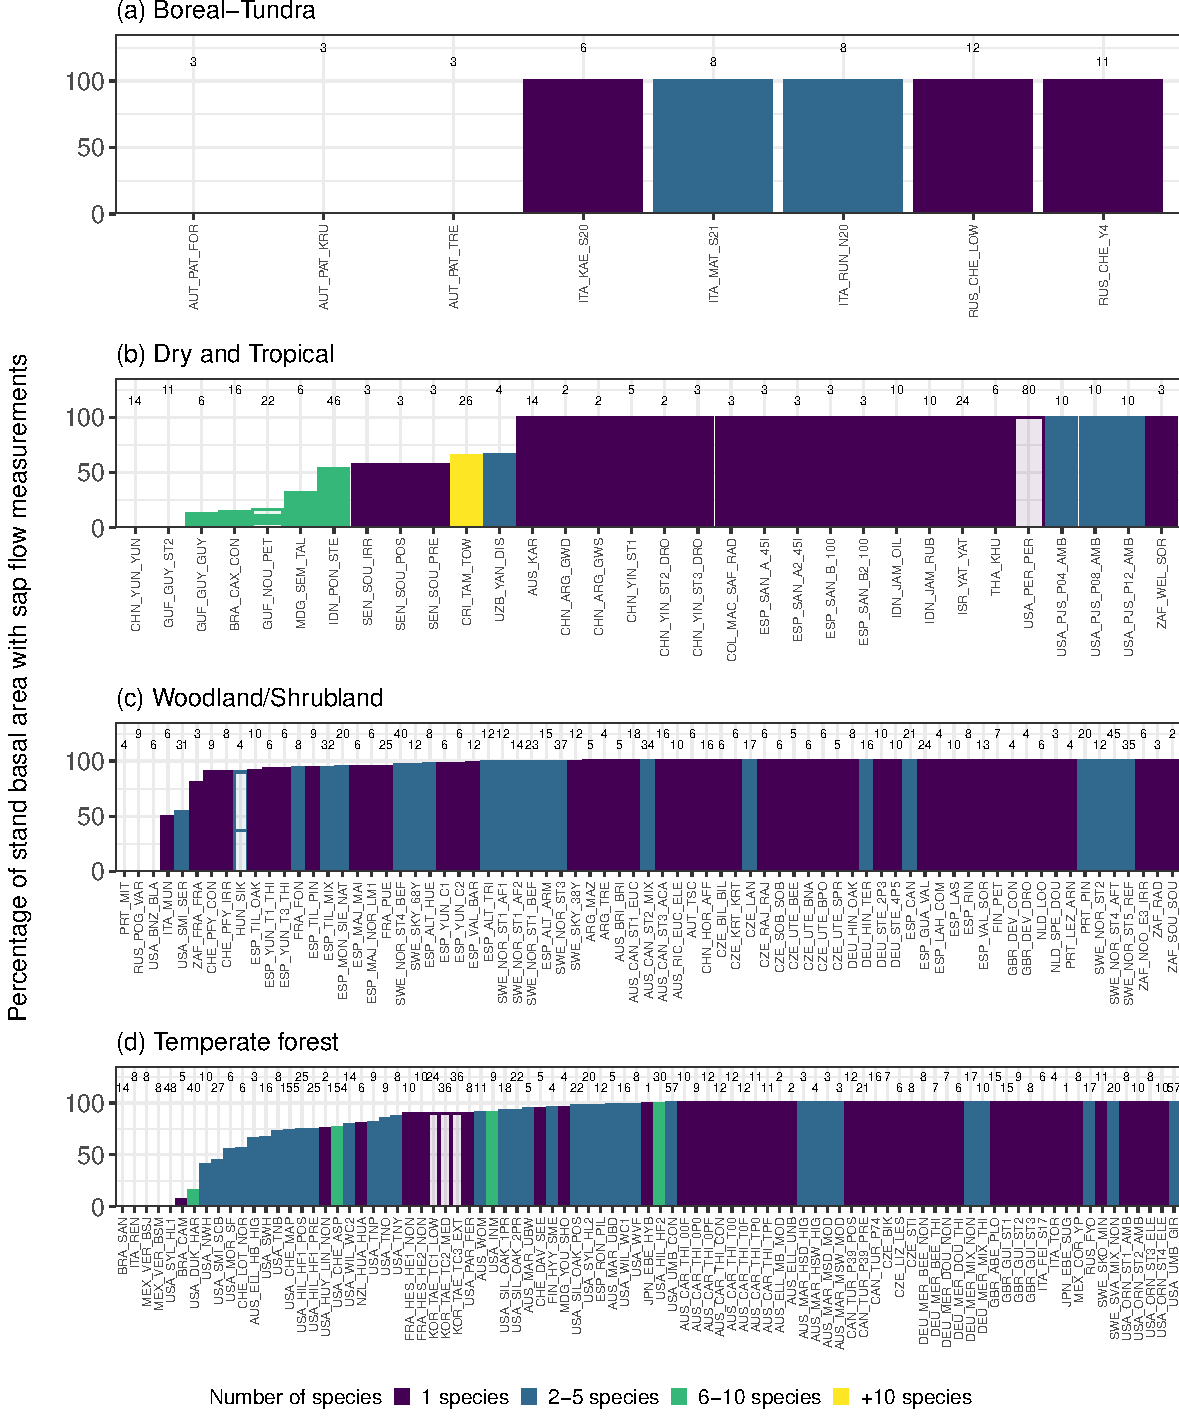
\includegraphics[width=1\linewidth]{figure/CH3/Figure9} 

}

\caption[Potential for upscaling species-specific plant sap flow to stand-level.]{Potential for upscaling species-specific plant sap flow to stand-level sap flow using SAPFLUXNET datasets. Datasets are shown using an aggregated biome classification; ‘Dry and Tropical’ include: ‘Subtropical desert’, ‘Temperate grassland desert’,‘Tropical forest savanna’ and ‘Tropical rain forest’. Each panel shows the percentage of total stand basal area that is covered by sap flow measurements for each species in the dataset. Datasets are also coloured by the number of species present. Numbers on top of each bar depict the total number of plants for a given dataset. Empty bars show datasets for which sap flow data expressed at the plant level were not available.}\label{fig:Ch2plot9}
\end{figure}
Stand-level transpiration estimates from a large number of SAPFLUXNET
sites can contribute to improve our understanding of the role of forest
transpiration in the context of stand water balance and its components
at the ecosystem (e.g.~Tor-ngern et al., 2018) and catchment levels
(Oishi et al., 2010; Wilson et al., 2001). Importantly, SAPFLUXNET can
contribute to better understand the global controls on vegetation water
use (Good et al., 2017), including the biological and climatic controls
on evapotranspiration partitioning into transpiration and evaporation
components (Schlesinger and Jasechko, 2014; Stoy et al., 2019). There is
some overlap between the FLUXNET network and SAPFLUXNET (47 datasets
from FLUXNET sites). Hence, transpiration from SAPFLUXNET can also be
used as a `ground-truth' reference for transpiration estimates from
remote sensing approaches (Talsma et al., 2018) and from eddy covariance
data (Nelson et al., accepted). Extrapolating sap flow-derived stand
transpiration to large spatial scales can be challenging due to
landscape-scale variation in forest structure (Ford et al., 2007) or
topography (Hassler et al., 2018), and to the low spatial
representativeness of sap flow measurements (Mackay et al., 2010). A
promising research avenue to help elucidate the role of vegetation in
driving hydrological changes across environmental gradients (Vose et
al., 2016) would be to combine species-specific stand transpiration data
from SAPFLUXNET with stand structural and compositional data from forest
inventories (e.g.~sapwood area index, Benyon et al., 2015).\par

Understanding the patterns and mechanisms underlying species
interactions with respect to water use within a community is necessary
to predict tree species vulnerability to drought (Grossiord, 2019).
Multispecies datasets from SAPFLUXNET (Table S4) can be used to assess
competition for water resources among species, for example by
identifying changes in seasonal water use across co-existing species and
hence characterizing the spatiotemporal segregation of their
hydrological niches (Silvertown et al., 2015). By providing a detailed
seasonal quantification of tree water use, SAPFLUXNET could also
complement isotope-based studies and contribute to interpret the large
diversity in root water uptake patterns observed worldwide (Barbeta and
Peñuelas, 2017; Evaristo and McDonnell, 2017) and to explain the
different seasonal origin of root-absorbed water across species and
environmental gradients (Allen et al., 2019).\par

Plant water fluxes and hydrodynamics are amongst the most uncertain
components of ecosystem and terrestrial biosphere models (Fatichi et
al., 2016; Fisher et al., 2018). These models are now incorporating
hydraulic traits and processes in their transpiration regulation
algorithms (Mencuccini et al., 2019), but multi-site assessments of
these algorithms are usually performed against evapotranspiration from
eddy flux data (Knauer et al., 2015; Matheny et al., 2014). Model
validation against sap flow data has been carried out typically in only
one (Kennedy et al., 2019; Williams et al., 2001) or few (Buckley et
al., 2012) sites. SAPFLUXNET can thus contribute to assess the
performance of models simulating transpiration of stands or species
within stands (e.g.~De Cáceres et al., submitted.), for a large number
of species and under diverse climatic conditions.\par

\section{Limitations and future
developments}\label{limitations-and-future-developments}

\subsection{Limitations}\label{limitations}

Sap flow data processing differs within and among methods, because
different algorithms, calibrations or parameters involved in sap flow
calculations may be applied. All of these methods contribute to
methodological uncertainty (Looker et al., 2016; Peters et al., 2018)
and this challenging methodological variability precludes the
implementation of a complete, standardised data workflow from raw to
processed data within SAPFLUXNET, as it is done for eddy flux data
(Vitale et al., 2020; Wutzler et al., 2018). Commercial software for sap
flow data processing from multiple methods is available
(i.e.~\url{http://www.sapflowtool.com/SapFlowToolSensors.html}) but it
has not yet been widely adopted. Freely available data-processing
software is only available for the HD method (Oishi et al., 2016;
Speckman et al., 2020; Ward et al., 2017).\par

Sap flow measured with thermometric methods provides a precise estimate
of the temporal dynamics of water flow through plants (Flo et al.,
2019). However, their performance in measuring absolute flows is mixed.
While some well-represented methods in SAPFLUXNET such as the CHP yield
accurate estimates (at least for moderate-to-high flows), the HD method,
the most represented method by far, can significantly underestimate
water flows (Flo et al., 2019). Because plant-level metadata contain
information that document the conversion from raw to processed data
(Appendix Table A5), a first-order correction for uncalibrated HD
measurements based on available methodological assessments can be
applied to allow intercomparability across methods. Nevertheless, given
the high unexplained variability (i.e.~by species and wood traits) in
the performance of sap flow calibrations (Flo et al., 2019), these
corrections should be applied with caution. The determination of zero
flow conditions (baselining) can also have significant impacts on the
quantification of absolute flow for several methods (Peters et al.,
2018; Smith and Allen, 1996; Steppe et al., 2010). The different
baselining approaches are also documented in the metadata to inform data
syntheses and/or to selectively apply correction factors.\par

SAPFLUXNET has been designed to store whole-plant sap flow data, and
therefore, sap flow measured at multiple points within an individual is
not available in the database. Even though this spatial variation could
be useful to describe detailed aspects of plant water transport
(Nadezhdina et al., 2009), focusing on plant-level data greatly
simplifies the data structure. Hence, SAPFLUXNET only includes data
already upscaled to the plant level by the data contributors. The main
details of how this upscaling process was done for each dataset are
provided together with other plant metadata (Table A5), but these
metadata show that within-plant variation in sap flow is often not
considered (Table 2). The impact of not accounting for radial and
circumferential variability when scaling single-point measurements of
sap flow to the whole-plant level can be important (Merlin et al.,
2020), but the estimation of sapwood area can also cause large errors
(Looker et al., 2016). SAPFLUXNET does not provide information on the
method employed to quantify sapwood area (e.g.~visual estimation with or
without the application of dyes, indirect estimation through allometries
at species or site levels) or on the accuracy of sapwood area data. This
precludes uncertainty estimation at the individual level. Future
developments in the SAPFLUXNET data structure could include this
information as metadata to better document the sensor-to-plant scaling
process.\par

While SAPFLUXNET makes global sap flow data available for the first
time, we note that spatial coverage is still sparse and some forested
regions are underrepresented in the database (Fig. 2a). We note
especially the relatively small number of datasets for boreal and
tropical forests, two important biomes in terms of global water and
carbon fluxes (Beer et al., 2010; Schlesinger and Jasechko, 2014). While
many geographic gaps are caused by the absence of sap flow studies from
such areas, some regions where sap flow studies have been conducted are
still not represented in SAPFLUXNET. For example, the recent
proliferation of Asian sap flow studies (Peters et al., 2018) has not
translated into a high representativity of Asian datasets in SAPFLUXNET
yet. Similarly, while the coverage of taxonomic and biometric diversity
is unprecedented, SAPFLUXNET lacks data for the extremely tall trees
(Ambrose et al., 2010) or for other growth forms such as shrubs (Liu et
al., 2011), lianas (Chen et al., 2015) and other non-woody species (Lu
et al., 2002).\par

\subsection{Outlook}\label{outlook}

The public release of SAPFLUXNET has set the stage for a first
generation of sap flow-based data syntheses. The work on these syntheses
will fuel new ideas and tools for future improvements of the database,
as for example new computing approaches for the processing and analysis
of sap flow datasets. One example would be the development of robust
imputation algorithms to gap-fill time series of sap flow and
environmental data, which can take advantage of tools and datasets
already developed by the ecosystem flux community (Moffat et al., 2007;
Vuichard and Papale, 2015). The dissemination of SAPFLUXNET will
encourage the use of machine-learning algorithms, only occasionally used
to analyse sap flow datasets so far (e.g.~Whitley et al., 2013). These
approaches can also be used to identify the relative importance of
different hydrometeorological drivers of transpiration (Zhao et al.,
2019), or to produce global transpiration maps, by combining SAPFLUXNET
with other data (Jung et al., 2019). This upscaling of stand
transpiration to large areas will also allow addressing broader
questions at the regional and continental scale, such as the role of
transpiration in moisture recycling (Staal et al., 2018).\par

The eventual success of this initiative, in terms of enabling data
reuse, contributing towards the understanding and modelling of tree
water use at local to global scales will likely encourage the sap flow
community to contribute new datasets to future updates of the database.
We expect that the development of open-source software for the
processing of sap flow raw data (Speckman et al., 2020), its eventual
widespread use by the sap flow community and the adoption of
standardized calibration practices will increase the quality and
intercomparability of future sap flow datasets. These new datasets will
hopefully expand the temporal, geographical and ecological
representativity of SAPFLUXNET when new data contribution periods can be
opened in the future.\par

\section{Data availability, access and
feedback}\label{data-availability-access-and-feedback}

In this paper we present SAPFLUXNET version 0.1.5 (Poyatos et al.,
2020a), which contains some small metadata improvements on version
0.1.4, the first one to be made publicly available, in March 2020. Both
versions supersede version 0.1.3 which was initially released to data
contributors in March 2019. The entire database can be downloaded from
its hosting webpage in the Zenodo repository
(\url{https://doi.org/10.5281/zenodo.3971689}, Poyatos et al. 2020a). In
this repository, we provide the database as separate .csv files and as
.RData objects; see section 2.4. for details on data structure. Together
with the initial publication of SAPFLUXNET in March 2019, we also
released the sapfluxnetr R package, available on CRAN, to enable easy
access, selection, temporal aggregation and visualisation of SAPFLUXNET
data. Feedback on data quality issues can be forwarded to the SAPFLUXNET
initiative email address:
\href{mailto:sapfluxnet@creaf.uab.cat}{\nolinkurl{sapfluxnet@creaf.uab.cat}}.
All the information about SAPFLUXNET, including the publication of new
calls for data contribution, can be found in the project website:
\url{http://sapfluxnet.creaf.cat/./par}

\section{Conclusion}\label{conclusion}

The SAPFLUXNET database provides the first global perspective of water
use by individual plants at multiple timescales, with important
applications in multiple fields, ranging from plant ecophysiology to
Earth-system science. This database has been built from
community-contributed datasets and is complemented with a software
package to facilitate data access. Both the database and the software
have been implemented following open science practices, ensuring public
access and reproducibility. Data sharing has been a key component of the
success of the FLUXNET network of ecosystem fluxes (Bond‐Lamberty,
2018), and many databases in plant and ecosystem ecology now offer open
data (Bond-Lamberty and Thomson, 2010; Falster et al., 2015; Gallagher
et al., 2020; Kattge et al., 2020). SAPFLUXNET fully aligns with this
philosophy. We expect that this initial data infrastructure will promote
data sharing among the sap flow community in the future (Dai et al.,
2018) and will allow the continued growth of the SAPFLUXNET database.

\chapter[Climate, functional traits and water use strategies]{Climate and functional traits jointly mediate tree water use strategies}

\setlength{\parindent}{0pt} Victor Flo, Jordi Martínez-Vilalta, Maurizio
Mencuccini1,3, Victor Granda, William R. L. Anderegg, Rafael Poyatos

\newpage

\setlength{\parindent}{30pt}

\section*{Abstract}

Tree water use is central to plant function and ecosystem fluxes.
However, it is still unknown how organ-level water relations traits are
coordinated to determine whole-tree water use strategies in response to
drought, and if this coordination depends on climate. Here we used a
global sap flow data base (SAPFLUXNET) to study the response of water
use, in terms of whole-tree canopy conductance (\(G\)), to vapour
pressure deficit (VPD) and to soil water content (SWC) for 142 tree
species. We investigated the individual and coordinated effect of six
water relations traits (vulnerability to embolism, Huber value,
hydraulic conductivity, turgor-loss point, rooting depth and leaf size)
on water use parameters, also accounting for the effect of tree height
and climate (mean annual precipitation, MAP). Reference \(G\) and its
sensitivity to VPD were tightly coordinated with water relations traits
rather than with MAP. Species with efficient xylem transport had higher
canopy conductance but also higher sensitivity to VPD. Moreover, we
found that angiosperms had higher reference \(G\) and higher sensitivity
to VPD than gymnosperms. Our results highlight the importance of trait
coordination and the complications of defining a single, whole-plant
resource use spectrum ranging from `acquisitive' to `conservative'.\par
\newpage

\section{Introduction}\label{introduction}

Plant water use is a key component of the global water cycle (Katul et
al., 2012). Plants regulate water use across a broad range of timescales
to maintain a favourable water status under varying water availability
(Feng et al., 2017). This regulation is the result of evolutionary
processes together with environmental and biophysical constraints that
have determined a huge diversity of species-specific water use
strategies mediated by a particular suite of traits (Bacelar et al.,
2012; Lu et al., 2020). These specific strategies determine plant
survival under drought (Mitchell et al., 2013), species coexistence
(Ehleringer et al., 1991; Jackson et al., 1995) and ecosystem CO2 and
water fluxes (Mencuccini et al., 2019a). Thus, a comprehensive
understanding of how regulation of whole-plant water use relates to
organ-level water relations traits would allow for a better
characterization of plant responses to drought and improved prediction
of climate change impacts on vegetation (Anderegg, 2015).\par

Among many other traits, the sensitivity of stomata to drought stress is
a major regulator of plant water use over relatively short timescales
(Martin-StPaul et al., 2017). In the absence of effective stomatal
control under drought, water uptake by roots might not compensate water
loss, resulting in high tensions in plants' vascular system, which can
trigger the entrance of air bubbles leading to xylem embolism (Tyree \&
Zimmermann, 2002). If embolism spreads to most of the xylem conduits,
water transport becomes restricted and plants may eventually die from
hydraulic failure (Tyree \& Sperry, 1988; Choat et al., 2018). Through
stomatal closure, plants reduce whole-plant canopy conductance (\(G\))
and therefore water loss and embolism risk, and maintain water status
within tolerable limits, at the expense, however, of reducing gas
exchange. Plants close stomata in response to drops in leaf and/or soil
water potentials (see Martínez-Vilalta \& Garcia-Forner, 2017) produced
by increased atmospheric water demand (i.e., vapor pressure deficit;
VPD) and reduced soil water availability (i.e., soil water content; SWC)
(Jarvis, 1976; Grossiord et al., 2017). Stomatal responses have been
largely described using semi-empirical models (Jarvis, 1976; Oren et
al., 1999; Damour et al., 2010) and optimality approaches relying on the
coupling of photosynthesis and transpiration (Wang et al., 2020), with a
recent focus on plant hydraulics (Sperry et al., 2016). Global syntheses
of these two approaches exist (Lin et al., 2015; Hoshika et al., 2018)
but they are only at the leaf level, and they do not consider the
coordination of stomatal and hydraulic traits.\par 

Coordination among stomatal sensitivity and other hydraulic and
allocation traits is thought to underlie differences in water use
strategies among species (Meinzer, 2002; Sperry et al., 2016; McCulloh
et al., 2019). Because in woody plants water has to be transported from
the soil through the xylem to supply leaf transpiration, the hydraulic
properties of the xylem are key determinants of plant water relations
and water use strategies. Particularly, maximum sapwood hydraulic
conductivity (\(K_s\); Table 1) and vulnerability to xylem embolism
(usually quantified as \(\Psi_{P50}\); i.e.~the water potential at which
half of \(K_s\) is lost) are key determinants of maximum transpiration
rates (Manzoni et al., 2013). In addition, a vulnerable xylem (i.e.~high
\textbar{}\(\Psi_{P50}\)\textbar{}) has been related to higher
canopy-level stomatal sensitivity to VPD across (Litvak et al., 2012)
and within some species (Aspinwall et al., 2011). \(K_s\) and
\(\Psi_{P50}\) have been hypothesized to define a safety-efficiency
trade-off at the tissue level, by which species with high \(K_s\) (i.e.,
high water transport efficiency) are also more vulnerable to embolism
(low \textbar{}\(\Psi_{P50}\)\textbar{} and low safety) and vice versa
(Venturas et al., 2017). However, this trade-off appears to be weak at
the global scale across species, at least as captured with current
measurement techniques (Gleason et al., 2016; Sanchez‐Martinez et al.,
2020). At the leaf level, another key component is the water potential
at turgor-loss point (\(\Psi_{TLP}\)), which is tightly associated with
drought tolerance and habitat water availability (Bartlett et al.,
2012). \(\Psi_{TLP}\) is also closely related to water potential at
complete stomatal closure (Brodribb \& Holbrook, 2003; Martin-StPaul et
al., 2017), and thus can be used as a proxy for quantifying the
sensitivity of plant water use to changes in water availability.\par

Allocation ratios between the organs involved in water loss, transport
and uptake are also important determinants of water use strategies. The
ratio of cross-sectional sapwood area to leaf area or Huber value
(\(Hv\)) is a major trait defining water use strategies because it
expresses the water conducting area per unit transpiring area. Increased
\(Hv\) can contribute to reduce water potential gradients within the
plant and therefore potentially compensate for a species vulnerable
xylem (Mencuccini et al., 2019b). In addition, a high \(Hv\) has also
been associated to strict stomatal control in conifers (Martínez-Vilalta
et al., 2004; Poyatos et al., 2007) and to higher reference canopy
conductance (Novick et al., 2009). Similarly, increasing rooting depth
(\(R_{depth}\)) gives access to deeper water sources, which potentially
allows maintaining less negative and stable water potentials as well as
supporting high water use even under climates with high evaporative
demand (Martínez-Vilalta \& Garcia-Forner, 2017). At the leaf level, the
importance of individual leaf size (\(L_s\)) for light penetration and
crown architecture has been thoroughly studied (Sellers, 1985), but its
influence on water use strategies has been little explored, despite the
role of leaf evaporative cooling for thermoregulation (Wright et al.,
2017). Large leaves with thick leaf boundary layers and an ineffective
stomatal control of water loss (Jarvis \& McNaughton, 1986), may need to
sustain higher transpiration rates to maintain leaf temperature within
operative limits under intense radiative heating and/or heat waves
(e.g.~Drake et al., 2018). This may lead to a trade-off between leaf
thermoregulation and the conservation of water and/or hydraulic function
(Fauset et al., 2018), especially in hotter sites (Aparecido et al.,
2020).\par

Water use strategies are also mediated by plant height, community
composition, and environmental conditions, particularly climate,
topography and soil properties; as well as spatial and temporal
variability in environmental conditions (Feng et al., 2018). Plant
height increases hydraulic path length and hydraulic resistance, and
thus plays a major role in the global coordination of several water use
traits such as \(\Psi_{P50}\) or \(K_s\) (Liu et al., 2019), \(Hv\)
(Mencuccini et al., 2019b) and reference canopy conductance (Novick et
al., 2009). Likewise, increasing tree height has been related to
enhanced sensitivity of canopy conductance to VPD for some species
(Schäfer et al., 2000). Because soil water is a common resource
belowground that is influenced by water uptake from many individuals and
species, the community composition and diversity of water use strategies
in an ecological community can also affect ecosystem fluxes and drought
progression (Anderegg et al., 2018, 2019). In addition, phylogeny may
constrain flexibility in water use strategies independently of the
environment, as it has been shown for example by the consistent
differences in hydraulic traits between angiosperms and gymnosperms
(Johnson et al., 2012; Bartlett et al., 2016) and by the strong
phylogenetic conservatism reported for some hydraulic traits such as
\(\Psi_{P50}\) and \(K_s\) at the global scale (Sanchez‐Martinez et al.,
2020).\par

In this study we explore water use strategies across tree species using
a trait-based approach, which provides a simplified framework to
understand species responses to drought at the global scale (Feng et
al., 2018). Our ultimate aim is to better understand how water use
strategies emerge from the covariation between traits and the influence
of climate. To that end, we use a global database of sap flow
measurements (SAPFLUXNET) to calculate whole-tree canopy conductance
(\(G\)) for 142 tree species growing on 126 sites. We then parameterize
the response of G to VPD and SWC at the species level and for major
taxonomic groups (i.e.~angiosperms and gymnosperms). Finally, we
characterize the relationships between water use traits and key
hydraulic and allocation traits among species (i.e. \(\Psi_{P50}\),
\(K_s\), \(Hv\), \(\Psi_{TLP}\), \(R_{depth}\), \(L_s\) and tree
height), controlling also for the climatic effects produced by
differences in precipitation. We hypothesize that (i) water use and
water relations traits are coordinated to determine water use strategies
at the species level, and (ii) species occupying drier habitats will
tend to be more `conservative' in their water use and also tend to have
drought tolerance traits. (iii) After controlling for climatic effects,
a safety-efficiency trade-off is visible at the scale of whole-plant
water use, as opposed to the scale of individual xylem conduits.\par

\section{Material and methods}\label{material-and-methods}

We took a two-step approach to test the previous hypotheses. First, we
modelled species-level whole-tree canopy conductance responses to
evaporative demand and soil water availability to obtain species' water
use parameters, taking advantage of a recently-compiled global sap flow
dataset. Next, we modelled the variability of those water use parameters
as a function of species' water relations traits, mean annual
precipitation (MAP), tree height and broad functional types (i.e.,
angiosperms and gymnosperms).\par

\subsection{Sap flow data}\label{sap-flow-data}

Data from 1929 trees belonging to 142 species on 126 plots without
experimental treatments (Table S1) and meeting data quality criteria
(see Data filtering section below) were obtained from the global
SAPFLUXNET database (Poyatos et al., 2020) (Fig. 1 and Table S2). For
each species-site combination, we extracted sub-daily sap flux density
(SFD; Table 1) or whole-tree sap flow (SF; 24 out of 126 data-sets) when
tree sapwood areas (ASW) were not available. For these datasets, SF data
were then transformed into SFD units by dividing SF values by tree ASW
estimated with an allometric relationship. This relationship was
obtained using all the SAPFLUXNET trees for which ASW data were
available and taking diameter at breast height (DBH) and functional type
(i.e., angiosperm or gymnosperm) as predictors (\(R^2\) = 0.78; n =
2262). Sub-daily SFD time-series were aggregated to daytime SFD averages
(i.e., 6am to 6pm solar time) using the sfn\_metrics function of the
sapfluxnetr R package (Granda et al., 2020). Time-series obtained from
non-calibrated thermal dissipation sensors were corrected for potential
bias in absolute SFD by applying a multiplier of 1.405, according to the
global synthesis of sap flow calibrations by Flo et al. (2019).\par

\subsection{Evaporative demand and soil water availability
data}\label{evaporative-demand-and-soil-water-availability-data}

We used vapour pressure deficit (VPD) and soil water content (SWC) as
proxies of evaporative demand and soil water availability, respectively.
Similar to SFD, VPD was obtained from on-site sub-daily measurements
from SAPFLUXNET averaged to daytime values. Soil water content (SWC;
v/v) was obtained from the 15-30 cm depth layer at 12 am from the
ERA5-land re-analysis product (Copernicus Climate Change Service (C3S),
2019) at 9x9 km resolution. We used ERA5-land re-analyses instead of
on-site SWC measures in order to maximize the number of plots and
species included in the study, since SWC data were missing in 44\% of
the SAPFLUXNET data-sets included in this study. In addition, ERA5-land
had longer time series (1980 to 2019). We validated the use of ERA5-land
data using a linear mixed-model (LMM) regression between ERA5-land and
on-site shallow SWC measurements by letting random intercepts and slopes
of the response vary by site (n observations = 32815; n plots = 71;
\(R^2\)conditional = 0.97, \(R^2\)marginal = 0.26).\par

To complement SWC, we also calculated relative extractable water (REW),
as a normalized measure of soil water availability, as follows:
\begin{equation}
REW_{j,i} = \frac{SWC_{j,i} - SWC_{min}}{SWC_{max} - SWC_{min}}
\end{equation}
where \(REW_{j,i}\) and \(SWC_{j,i}\) are plot (\(j\)) daily (\(i\))
values, and SWCmax and SWCmin, the overall maximum and minimum SWC
measured at a plot, respectively. REW takes values between 0 and 1,
being 0 the absolute plot lowest SWC and 1 being the highest.\par

\subsection{Data filtering}\label{data-filtering}

We restricted the analysis to periods without potential phenological
changes in leaf area to minimize variations in conductance unrelated to
VPD and SWC changes. In the absence of detailed plot-specific
observations, we excluded all data for periods comprised between 15 days
prior to the first day with temperatures below 0ºC and 30 days following
the last day under 0ºC, respectively, during the cold seasons of each
plot site (similarly to Novick et al., 2016). To prevent potential
artefacts due to unstable weather conditions in the calculation of
whole-tree canopy conductance (Ewers \& Oren, 2000) or in the estimation
of model parameters, we filtered out days when SWC increased (rainy
days), as well as days when daytime-averaged VPD was below 0.3 kPa
(Anderegg et al., 2018). To ensure sufficiently contrasting conditions
of evaporative demand and soil water availability, we also discarded
species with both VPD ranges below 0.5 kPa and SWC ranges below 0.05 (n
= 8 species).\par

After data filtering, the study covers a large geographic area ‒being
Europe and the east of North America especially well represented (Fig
1)‒ and a wide range of climate conditions, with MAP values ranging from
14 mm to 3626 mm (mean \textbackslash{}pm SD = 953 mm \textbackslash{}pm
545 mm). Out of the 142 species used in the analyses, 116 were
angiosperms and 26 gymnosperms. The number of trees per species ranges
from 215 trees (Pinus sylvestris) to 1 (this being the case for 23
species) (Table S2). Tree species-level heights (H) range from 2 m
(Coprosma quadrifida) to 40 m (Carya glabra) (mean \textbackslash{}pm SD
= 21 m \textbackslash{}pm 9.75 m).\par

\subsection{Whole-tree canopy conductance
calculation}\label{whole-tree-canopy-conductance-calculation}

Daytime SFD was transformed from
{[}\(cm^3 \: cm_{Asw}^{-2} \: h^{-1}\){]} to
{[}\(kg \: m_{Asw}^{-2} \: s^{-1}\){]} and converted to daily whole-tree
canopy conductance normalized per unit of sapwood area \(G_{Asw}\) using
Phillips and Oren (1998) and unit transformations (eq.2).
\begin{equation}
G_{Asw,j,i,k} = \frac{115.8 + 0.4236 \: T_{j , i} \cdot SFD_{j , i , k}}{VPD_{j,i}}\cdot 44.6 \cdot \frac{273}{(273 + T_{j,i})} \cdot \frac{101.325 \: e^{0.00012 \cdot h_i}}{101.325}
\end{equation}
Where \(SFD_{j,i,k}\) is sap flux density value of each plot (\(j\)),
day (\(i\)), and tree (\(k\)); \(T_{j,i}\) is the temperature,
\(VPD_{j,i}\) is the daytime vapor pressure deficit and \(h\) is the
altitude of each plot site. When h was not available it was obtained
from The Shuttle Radar Topography Mission (SRTM) (Earth Resources
Observation And Science (EROS) Center, 2017) (n = 2 plots).\par

The conductance obtained using eq. 2 is considered a good proxy of the
tree-level stomatal conductance under the assumption that the canopy and
the atmosphere are well-coupled, i.e., when the aerodynamic conductance
is much larger than the stomatal conductance. Although this is generally
assumed in sap flow studies for both needleleaf and even broadleaf
species, there is evidence that coupling may only be partial in some
cases (Magnani et al., 1998; De Kauwe et al., 2017). Therefore, we also
calculated whole-tree stomatal conductance (\(G_{Asw}^{'}\)) by removing
the contribution of aerodynamic conductance in a subset of plots-species
(n plots = 64; n species = 47) where wind speed data were available in
SAPFLUXNET (see supplementary material for details, Chu et al., 2018;
Tan et al., 2019). We also related the environmental sensitivity of
\(G_{Asw}^{'}\) to the hydraulic and allocation traits (see Statistical
analyses section below) to assess the potential impact of partial
canopy-atmosphere coupling on our results.\par

\subsection{Traits and climatic data}\label{traits-and-climatic-data}

Species-level traits (\textbar{}\(\Psi_{P50}\)\textbar{}, \(Hv\),
\(K_s\), \textbar{}\(\Psi_{TLP}\)\textbar{}, \(R_{depth}\) and \(L_s\))
were taken from HydraTry (Mencuccini et al., 2019b; Sanchez‐Martinez et
al., 2020) and the Global Leaf Size Dataset (Wright et al., 2017) (Table
S2). \textbar{}\(\Psi_{P50}\)\textbar{}, \[Hv\], \(K_s\) and \(L_s\)
were log-transformed to achieve normality. In addition, we obtained tree
species-level height (H) as the average of SAPFLUXNET actual tree
heights, with the number of tree-days with available sap flow values as
weighting factor. The height of the stand was used when the actual
height of a tree was not available (792 out of 1929 trees).\par

To account for climatic effects on the species' water use parameters and
on water relation traits, we used mean annual precipitation (MAP), mean
annual temperature (MAT) and an aridity index defined as precipitation
over potential evapotranspiration (PPET) (Fig. 1, Fig. S6, Fig. S7).
However, for simplicity, we only included MAP in the analyses since for
the species in the study MAP was strongly correlated with PPET (\(r\) =
0.94) and MAT (\(r\) = 0.76), whereas PPET and MAT correlation was lower
(\(r\) = 0.56). MAP and MAT were obtained for all study plots from the
CHELSA data set (1x1 km resolution) (Karger et al., 2017) and averaged
at the species level weighting by the number of tree-days. PPET were
obtained from CGIAR-CSI Global Aridity index (Trabucco \& Zomer,
2019).\par

\subsection{\texorpdfstring{\(G_{Asw}\) sensitivity to soil water
availability and water
demand}{G\_\{Asw\} sensitivity to soil water availability and water demand}}\label{g_asw-sensitivity-to-soil-water-availability-and-water-demand}

In some species, \(G_{Asw}\) measurements were distributed very
heterogeneously throughout the range of VPD or SWC. To avoid the issues
associated with such unbalanced distributions we used binned data.
Specifically, we calculated the average of \(G_{Asw}\) measurements
comprised into 0.2 kPa VPD intervals and five bins spanning the
plot-species specific SWC range. For each summarized \(G_{Asw}\) we
defined a characteristic VPD and SWC as the average values of VPD and
SWC of the data in the bin. The summarized values of \(G_{Asw}\) were
fitted using LMM as a function of the logarithm of VPD (ln(VPD)) and the
logarithm of SWC (ln(SWC)) as additive explanatory variables using
uncorrelated random slopes for each species and a random intercept for
each tree nested in each species. We log-transformed the independent
variables to linearise the relationships and ensure normal residuals.
LMMs were fitted using the lmer function from the lme4 R package (Bates
et al., 2015). Using the coef function from lme4 we obtained species
parameters \(\beta_{VPD}\) and \(\beta_{SWC}\) (i.e.~species \(G_{Asw}\)
sensitivity to VPD and to SWC, respectively), with higher values of
\(\beta_{VPD}\) or \(\beta_{SWC}\) meaning stronger G reductions with
increasing VPD or decreasing SWC, respectively. In addition, a reference
\(G_{Asw}\) (\(G_{REF}\)) characterizing water use under standard
conditions for each species, was predicted setting VPD = 1 kPa and SWC =
0.5 m3 m-3 (which is close to the average maximum of all sites).
Complementary models were also fitted following the same procedure but
with REW instead of SWC, so that soil water content variability was
normalized across sites. Additional models were also fitted using canopy
stomatal conductance (\(G_{Asw}^{'}\)) as response variable. Finally, to
remove parameter outliers, species with \(G_{REF}\) , \(\beta_{VPD}\) or
\(\beta_{SWC}\) outside the 99.9 percentile of their normal distribution
were excluded from subsequent analyses (2 out of 142 species
excluded).\par

\subsection{Statistical analyses}\label{statistical-analyses}

We tested whether water use regulation traits (\(G_{REF}\),
\(\beta_{VPD}\) and \(\beta_{SWC}\)) differ between angiosperms and
gymnosperms using a simple linear model. Next, we constructed bi-variate
linear relationships between species' fitted parameters and species'
water relations traits. Furthermore, we repeated these linear
relationships by adding MAP and H as predictors and applying a stepwise
model selection, to discern whether the effect of the traits remained
significant once these new variables were added to the model. In all the
analyses we used the number of species' tree-days as a weighting
factor.\par

Finally, we performed a path analysis using the SEM function of the
lavaan R package (Rosseel, 2012). Path analysis accounts for direct and
indirect dependencies among variables. To account for the coordinated
effect of the species' relations traits and to maximize the number of
species (106 species), we imputed species' trait missing values (Table
S2) using the imputePCA function of the package missMDA (Josse \&
Husson, 2016) and then performed a Principal Component Analysis (PCA) to
extract the two main principal components (Fig. S1). A single path model
was built including the three parameters describing \(G_{Asw}\)
behaviour (\(G_{REF}\), \(\beta_{VPD}\) and \(\beta_{SWC}\)) as response
variables and using MAP, \(H\) and the two dimensions of the traits' PCA
as explanatory variables. In addition to direct relationships, indirect
effects of MAP and \(H\) on the fitted parameters were also included
through their effect on the PCA dimensions (Liu et al., 2019). We also
accounted for the effect of MAP on \(H\). We included the number of
tree-days per species as a weighting factor in the model. We performed a
model selection procedure to include only paths with at least moderately
strong support (P \textless{} 0.1). Finally, we also checked that the
fit of the final model was not significantly different from the
saturated model using the lavTestLRT function of the lavaan R package
(Rosseel, 2012) with Satorra and Bentler (2001) approximation. All
variables were standardized before fitting the path models. All the
analyses of the study were performed in R3.6.1 (R Core Team, 2018).\par

\section{Results}\label{results}

\subsection{Water use parameters and differences between angiosperms and
gymnosperms}\label{water-use-parameters-and-differences-between-angiosperms-and-gymnosperms}

The model used to obtain water use parameters explained a 59.8\% of the
total conditional variance in the original data. Reference conductance
(\(G_{REF}\)) across species ranged between 82.4
\(mol\: m{Asw}^{-2}\: s^{-1}\) (Juniperus monosperma) and 333
\(mol\: m{Asw}^{-2}\: s^{-1}\) (Acacia longifolia), \(\beta_{VPD}\)
between -26 \(mol\: m{Asw}^{-2}\: s^{-1}\) (Avicennia marina) and 306
\(mol\: m{Asw}^{-2}\: s^{-1}\) (Ulmus americana) and \(\beta_{SWC}\)
between -17.3 \(mol\: m{Asw}^{-2}\: s^{-1}\) (Acer saccharum) and 112
\(mol\: m{Asw}^{-2}\: s^{-1}\) (Acacia longifolia) (Fig. S2 -- S3 --
S4). Most species showed declining G with increasing VPD (positive
\(\beta_{VPD}\)) and increasing G with increasing SWC (positive
\(\beta_{SWC}\)).\par

Species showing opposite responses were two temperate (Acer saccharum,
Quercus petraea), one tropical (Ampelocera macrocarpa) and a mangrove
(Avicennia marina) species that showed negative sensitivities to one of
the variables (Fig. S2). Mean \(G_{REF}\) and \(\beta_{VPD}\) were
significantly higher for angiosperms than for gymnosperms (Fig. 2).
However, there were no differences in \(\beta_{SWC}\) between
angiosperms and gymnosperms. Across all species (including angiosperms
and gymnosperms), \(G_{REF}\) and \(\beta_{VPD}\) were strongly and
positively correlated (\(r\) = 0.75; with a weighted slope of 0.67; Fig.
S5), being the species with high \(G_{REF}\) more sensitive to VPD, but
strong correlations were not found between \(G_{REF}\) and
\(\beta_{SWC}\) or between \(\beta_{VPD}\) and \(\beta_{SWC}\)
(\textbar{}\(r\)\textbar{} \textless{} 0.34 in both cases). When
comparing water use parameters calculated considering and not
considering aerodynamic conductance, we found that \(G_{REF}\) was
strongly correlated to \(G_{REF}^{'}\) (\(r\) = 0.8); however,
\(\beta_{VPD}\) and \(\beta_{VPD}^{'}\) were poorly correlated (\(r\) =
0.26) while \(\beta_{SWC}\) and \(\beta_{SWC}^{'}\) showed no
significant correlation.\par

\subsection{Coordination with hydraulic and allocation
traits}\label{coordination-with-hydraulic-and-allocation-traits}

In the bi-variate models relating \(G_{REF}\) with hydraulic and
morphological traits, we found that \(G_{REF}\) showed a negative
relationship with \textbar{}\(\Psi_{P50}\)\textbar{}, \(Hv\) and
\textbar{}\(\Psi_{TLP}\)\textbar{} (Table 2 and Fig. 3a,c,d), whereby
species more resistant to embolism, with higher allocation to the
sapwood relative to leaves and with more negative turgor-loss pressures
showed lower \(G_{REF}\). Furthermore, \(G_{REF}\) was positively
related to \(K_s\), \(R_{depth}\) and \(L_s\) (Table 2 and Fig. 3b,e,f),
with species with efficient xylem, deeper roots and bigger leaves
showing higher \(G_{REF}\). For these traits, \(L_s\) was the one
explaining the largest fraction of \(G_{REF}\) variability (\(R^2\) =
0.39). With the exception of \(\Psi_{TLP}\), these relationships
remained significant also for \(G_{Asw}^{'}\) (Table S3).\par

\(\beta_{VPD}\) was negatively related with
\textbar{}\(\Psi_{P50}\)\textbar{} and \(Hv\) and positively with
\(K_s\) (Table 2 and Fig. 4a,b,c), i.e., species with less safe and more
efficient xylem present higher sensitivity to VPD, and hence more strict
stomatal control as atmospheric water demand increases. \(\beta_{VPD}\)
was also positively related to \(R_{depth}\) and \(L_s\) (Table 2 and
Fig. 4e,f), indicating that deeper roots and larger leaves were
associated to higher stomatal sensitivity to VPD. Absolute turgor-loss
point (\textbar{}\(\Psi_{TLP}\)\textbar{}) was weakly negatively related
with \(\beta_{VPD}\) (p value = 0.093; Table 2). \(Hv\) and \(L_s\) were
the traits explaining most of \(\beta_{VPD}\) variability (\(R^2\) =
0.36 and \(R^2\) = 0.33, respectively). With the exception of
\(\Psi_{TLP}\), these relationships remained significant also for
\(G_{Asw}^{'}\) (Table S3).\par

\(\beta_{SWC}\) was positively related to
\textbar{}\(\Psi_{P50}\)\textbar{} and \(Hv\) (Table 2 and Fig. 5a,c),
i.e., species with higher resistance to embolism and larger ratios of
sapwood to leaf area were more sensitive to soil water depletion. In
addition, species with larger leaves (\(L_s\)) and, marginally (p value
= 0.095), with deeper roots (\(R_{depth}\)) were less sensitive to soil
water stress (Table 2 and Fig. 5e,f). In general, water relations traits
explained a lower proportion (at most 9\%) of the variability in
\(\beta_{SWC}\) than of \(G_{REF}\) or \(\beta_{VPD}\). However, we
should treat relationships between \(\beta_{SWC}\) and
\textbar{}\(\Psi_{P50}\)\textbar{}, \(Hv\) and \(R_{depth}\) with
caution, since they all become non-significant when aerodynamic
conductance was taken into account (Table S3) or when REW was used
instead of SWC (Table S3). Furthermore, when REW was used instead of
SWC, all soil moisture sensitivity-trait relationships became
non-significant (Table S4).\par

Ecological factors associated with water use parameters and coordination
When the coordination between water use parameters and water relations
traits was assessed while also accounting for the effects of MAP (mean
annual precipitation) and \(H\) (tree species-level mean height), most
of the relationships described in the previous section remained
significant, with only three exceptions. The relationships that were no
longer observed corresponded to the effect of \(\Psi_{TLP}\) on
\(G_{REF}\) and the effects of \textbar{}\(\Psi_{P50}\)\textbar{} and
\(Hv\) on \(\beta_{SWC}\) (Table 3). In these models, MAP was the
variable that explained most of the variability in stomatal responses to
soil water (\(\beta_{SWC}\)), with generally lower sensitivity to SWC in
locations with high MAP (Table 3), although this effect reversed in the
\(L_s\) model. However, when models were calculated using
\(\beta_{SWC}^{'}\), MAP effects were all negative (Table S5). On the
other hand, MAP was largely unrelated to \(G_{REF}\) and \(\beta_{VPD}\)
in most of the \(G_{REF}\) and \(\beta_{VPD}\) models (Table 3).
Finally, our results show that taller trees tend to have higher
\(G_{REF}\) and higher sensitivity to VPD (\(\beta_{VPD}\)), however,
when \(G_{REF}\) was obtained from \(G_{Asw}^{'}\) (i.e.
\(G_{REF}^{'}\)), \(H\) was not selected in the final models (Table S5).
The relationship between \(H\) and soil drought sensitivity
(\(\beta_{SWC}\)) was less clear, since it was significantly negative in
only two of the models (Table 3), suggesting higher sensitivity to soil
drought in shorter trees. However when aerodynamic coupling was taken
into account, the relationship was inverted and taller trees had higher
sensitivity to SWC (Table S5).\par

The two main dimensions of the PCA analyses describing water relations
trait coordination explained a 69.8\% of the total variance (Fig. S1).
The primary PCA dimension (Dim1; 56.8\% of variance) could be
interpreted as a safety-efficiency trade-off axis, whereby positive
values are related to elevated \(K_s\), large \(L_s\), deep roots, low
\(Hv\) and low \textbar{}\(\Psi_{P50}\)\textbar{}. The second PCA
dimension (Dim2; 13\% of variance) was associated to leaf turgor-loss
pressure (\(\Psi_{TLP}\)), with positive values related to high
\textbar{}\(\Psi_{TLP}\)\textbar{} levels and, to a lower extent, deeper
roots.\par

In the path analyses, efficiency traits (positive PCA Dim1 values) were
significantly related to high annual precipitation (high MAP) and to
taller trees (large \(H\)) (Fig. 6). Also, \(H\) increased with MAP.
\(G_{REF}\) was positively associated with Dim1 (Fig. 6) and taller
trees also had marginally higher \(G_{REF}\) (Fig. 6). Similarly, higher
\(\beta_{VPD}\) (i.e., higher VPD sensitivity) was positively related to
efficient water transport (Dim1) and to \(H\) (Fig. 6). Sensitivity to
SWC (\(\beta_{SWC}\)) showed a marginal, negative relationship with
Dim1, so that sensitivity increased with xylem resistance to embolism
(Fig. 6). Finally, \(G_{REF}\) co-varied positively with \(\beta_{VPD}\)
and \(\beta_{SWC}\), implying that as \(G_{REF}\) increases so do
\(\beta_{VPD}\) and \(\beta_{SWC}\) (Fig. 6, Fig. S5). The second
dimension of the PCA was not included in the final path model,
suggesting a lack of coordination between \(\Psi_{TLP}\) and water use
parameters.\par

\section{Discussion}\label{discussion}

In this study, we present a novel analysis linking organ-level traits
with whole-plant water use strategies at the global scale, made possible
by the compilation of the first global sap flow database. We provide
evidence of a coordination between water relations traits and water use
parameters (\(G_{REF}\), \(\beta_{VPD}\) and \(\beta_{SWC}\)), while
accounting for the effects of climate and tree size. Some water use and
trait associations were explained by climate affiliations of species,
but most relationships between water use and water relations traits
remained after accounting for climate and tree size effects. As any
synthesis effort of this magnitude based on diverse data sources, our
study presents several limitations. First, sap flow data used to
estimate G carry some uncertainty issues, although these may be less
relevant for assessing environmental responses as we do here than for
characterizing absolute values (Flo et al., 2019). Second, SAPFLUXNET
may have an incomplete coverage of global forest ecosystems (Fig. 1,
Poyatos et al., 2020). Third, highly non-linear or threshold-based SWC
responses may be difficult to capture, especially when having to resort
to reanalysis data. Fourth, other ecological processes such as partial
canopy-atmosphere coupling or intra-specific variability in traits
and/or water use regulation may influence our results.\par

\subsection{Climate influence on water use strategies across
species}\label{climate-influence-on-water-use-strategies-across-species}

Our results showed no direct effect of mean annual precipitation (MAP)
on \(G_{REF}\) and \(\beta_{VPD}\), but instead indirect MAP effects on
water use strategies mediated through hydraulic and allocation traits
(Fig 6 and Fig. S6), suggesting that MAP constrains feasible water
relations traits (Bourne et al., 2017; Liu et al., 2019), which then
directly determine water use rate and \(\beta_{VPD}\). The direction of
these effects is consistent with previous studies showing that
\(\beta_{VPD}\) increased with aridity in rainforest species
(Cunningham, 2004; but see Grossiord et al., 2019) and at continental
scales across ecosystems and functional types (Novick et al., 2016), but
these studies did not disentangle direct from indirect effects. Although
the global controls on \(\beta_{SWC}\) were less clear in our analyses,
in part due to the influence of aerodynamic coupling (cf.~Table 3 and
S5), climate effects on this variable also appeared to be largely
indirect (Fig. 6). Therefore, our results underscore the importance of
using water relations traits, rather than climate when addressing
species whole-tree water use strategies and ecosystem flux sensitivities
to VPD.\par

\subsection{Water use parameters}\label{water-use-parameters}

Water use parameters differed widely among species (Fig. S2) and defined
a gradient of water use sensitivities to drought stress. Within the
gradient of parameters, angiosperms and gymnosperms showed distinct
whole-plant water use strategies (Fig. 2). We found that gymnosperms
have generally more `conservative' water use strategies in terms of
lower \(G_{REF}\) but not in terms of enhanced sensitivity to VPD or
SWC. Similarly, previous studies also showed lower sensitivity to VPD in
gymnosperms compared to angiosperms (Johnson et al., 2012; Lin et al.,
2015), which could be associated to higher safety margins (Choat et al.,
2012; Anderegg et al., 2016). The `conservative' \(G_{REF}\) strategy of
gymnosperms could be explained by group-specific trait syndromes
associated to water relations traits (Fig. S8), wood anatomy (Venturas
et al., 2017), and lower photosynthetic rates, stomatal conductance or
leaf N concentrations (Lusk et al., 2003).\par

\(G_{REF}\) and \(\beta_{VPD}\) showed a strong positive correlation
across species (Fig. S5) similar to the one found by Oren et al. (1999).
This implies stronger VPD control on transpiration in species with
higher water use under optimal conditions (higher \(G_{REF}\)). However,
our global cross-species analyses might mask finer variations, as
\(\beta_{VPD}\) (or \(\beta_{VPD}\) / \(G_{REF}\)) is expected to be
lower across species from dry sites (Oren et al., 1999) or along a
decreasing gradient of SWC within species (Domec \& Johnson, 2012; Zhang
et al., 2012; but see Poyatos et al., 2007). Nevertheless, this result
suggests that \(G_{REF}\) can be a suitable proxy of whole-tree canopy
conductance sensitivity to VPD, as it is at the leaf (Oren et al., 1999)
or ecosystem (Grossiord et al., 2020) levels.\par

The lack of correlation found between the sensitivity to SWC calculated
with and without aerodynamic conductance, indicates that canopy coupling
could be important in calculating \(\beta_{SWC}\) and that in order to
predict and model plant water responses to soil water dynamics, we
likely have to explicitly consider aerodynamic and boundary layer
conductances. In addition, these land-atmosphere interactions might be
crucial in diagnosing and modelling the soil moisture controls over
other ecosystem processes such as the carbon cycle (Green et al., 2019;
Kannenberg et al., 2020).\par

\subsection{Coordination between water use parameters and water
relations
traits}\label{coordination-between-water-use-parameters-and-water-relations-traits}

Our results support the hypothesis of a strong coordination between
\(G_{REF}\) and individual hydraulic and allocation traits. \(G_{REF}\)
aligns with `efficiency' traits (\(K_s\)) in the hydraulic
safety-efficiency axis, and is thus negatively related to `safety'
traits (particularly \(\Psi_{P50}\)). These results are consistent with
the overall proposed coordination between plant hydraulics and gas
exchange (Meinzer, 2002; Sperry et al., 2002; Mencuccini, 2003; Maherali
et al., 2006; Henry et al., 2019) and with the notion that species
operate close to their maximum transport capacity sustained by their
hydraulic system (Manzoni et al., 2013). Large individual leaf areas
were also related to higher \(G_{REF}\), probably due to higher leaf
hydraulic conductance mediated by wider conduits (Schreiber et al.,
2016; Ding et al., 2020). The positive association of elevated
\(G_{REF}\) with deeper roots points out the requirement of deep rooting
to supply water for keeping high transpiration rates, and is also found
in the coordination between \(R_{depth}\), \(\Psi_{P50}\) and \(K_s\)
(Mursinna et al., 2018).\par

Coordination between whole-tree water use sensitivity to VPD
(\(\beta_{VPD}\)) and to SWC (\(\beta_{SWC}\)) with organ-level water
relations traits had not been assessed before at a global scale. All the
studied water relations traits (except \(\Psi_{TLP}\)) appear to be
related to \(\beta_{VPD}\), whereby the species with more `efficient' or
less ``safe'' traits tend to be those which show higher \(\beta_{VPD}\).
These results are consistent with previous studies relating stomatal
responses and water relation traits (Lu et al., 2020) and with the
stomatal gas exchange optimization theory (see Tyree \& Sperry, 1988;
Wang et al., 2020). By contrast, after controlling for climate and tree
height, conductance sensitivity to SWC (\(\beta_{SWC}\)) was only
(negatively) related to \(L_s\). Notably, \(\beta_{SWC}\) was unrelated
to \(\Psi_{TLP}\), in contrast to Maréchaux et al. (2018), that
evidenced more negative \(\Psi_{TLP}\) related to lower reductions in
sap flow with decreasing SWC. This absence of relationship, including
the weak \(\beta_{VPD}\) ‒ \(\Psi_{TLP}\) correlation, could be
attributed to noise and uncertainty in \(\Psi_{TLP}\) measures (Meinzer
et al., 2014) or with \(\Psi_{TLP}\) plasticity (Bartlett et al., 2012;
Rosas et al., 2019). In addition, the lack of relationship between
\(\beta_{SWC}\) and \(R_{depth}\) could be explained by the complexity
of rooting depth dependency on soil water infiltration, tree height and
climate (Fan et al., 2017).\par

We also explored the coordinated effect of water relations traits on
water use parameters and accounted for direct and indirect climate and
tree height effects through the PCA and the path model. Based on our
results, water use strategies would be, in terms of \(G_{REF}\),
consistent with the Reich (2014) notion of a whole-plant resource use
spectrum, ranging from `conservative' to `acquisitive' species. However,
in terms of absolute sensitivity to VPD, our results go against this
idea, since acquisitive species (with high \(G_{REF}\)) are also more
sensitive to VPD (more `conservative'). Therefore, our study would
support a more physiological interpretation of water use strategies that
stresses trait coordination. According to this interpretation, plants
with `safer' hydraulic systems (high resistance to embolism) are able to
function at higher water tensions without requiring a strict water use
regulation, implying that they can show a more `acquisitive' regulation
of water use so that they can benefit from having a wider range of
conditions to operate safely. In other words, high transport capacity in
the xylem (\(K_s\)) is associated with high canopy conductance
(\(G_{REF}\)) and a vulnerable (sensitive) xylem is also associated with
a stricter regulation of gas exchange. However, a vulnerable xylem
reduces safety, and is usually interpreted as part of an `acquisitive'
strategy, whereas a strict regulation of water use prevents hydraulic
failure and hence corresponds to a `conservative' strategy. This view is
also consistent with the positive relationship between \(\Psi_{P50}\)
and \(\Psi_{TLP}\), even if it saturates at relatively low water
potentials (cf.~Martin-StPaul et al., 2017). These results highlight the
complications of defining a single, whole-plant resource use spectrum
ranging from `acquisitive' to `conservative' species (sensu Reich,
2014), and points to the need of considering different organs and
functional axes when assessing whole-plant functional integration.\par

Regarding tree's height, it was coordinated directly and indirectly
‒through water relations traits‒ with water use parameters (Table 3 and
Fig. 6), in a way that taller trees displayed more `efficient' water use
strategies. Alignment of water relations traits and \(H\) was consistent
with results found by Liu et al. (2019), relating maximum plant size
with \(\Psi_{P50}\), \(K_s\) or \(Hv\) at the global scale across
species and life forms. These complex direct and indirect \(H\)
relationships might be driven by ecosystem water availability (Fig. 6)
and low freezing risk (Olson et al., 2018), which allows for increased
water use through efficient water transport (e.g.~high \(K_s\) or
\(Hv\)), compensating the increase of resistance due to the enlarged
water path of taller trees (Barnard \& Ryan, 2003; Liu et al., 2019;
Mencuccini et al., 2019b). Furthermore, \(H\) could also affect
differential sensitivity to VPD and SWC in tall trees (Giardina et al.,
2018), as their canopy would be more exposed to VPD, requiring higher
\(\beta_{VPD}\), and would potentially have more developed root systems,
which would decrease \(\beta_{SWC}\).\par

\subsection{Conclusions}\label{conclusions}

Understanding tree water use strategies at the global scale is crucial
to better predict ecosystem water cycles and drought vulnerability of
species and ecosystems. Here we demonstrate that there is a global
spectrum of water use strategies determined by the coordination of
hydraulic and allocation traits, rather than by climate. In particular,
species-specific \(G_{REF}\) and \(\beta_{VPD}\) (but not
\(\beta_{SWC}\)) are closely related to the species-specific water
relations traits. We have also shown significant differences between
angiosperm and gymnosperm water use strategies, showing greater water
use and sensitivity to VPD in angiosperms than gymnosperms, a finding
that could be related to distinct water relations traits syndromes (Fig.
S8). Our trait-based approach allowed for a simplified global mapping of
water use strategies. The use of simple measurable traits (e.g.~leaf
size) altogether with functional grouping can lead to a better
approximation of species reference water conductance and its sensitivity
to VPD. Recently developed global maps of traits (Moreno-Martínez et
al., 2018; Trugman et al., 2020) would permit the inclusion of such
water use strategies in Land Surface and Earth System Models potentially
improving ecosystem carbon and water fluxes predictions.\par

\chapter*{References}\label{references}
\addcontentsline{toc}{chapter}{References}

\setlength{\parindent}{-0.20in} \setlength{\leftskip}{0.20in}
\setlength{\parskip}{8pt}

Abeli, T. et al. 2014. Effects of marginality on plant population
performance. - J. Biogeogr. 41: 239--249.\par
Ackerly, D. D. 2003. Community Assembly , Niche Conservatism , and
Adaptive Evolution in Changing Environments. - Int. J. Plant Sci. 164:
164--184.\par
Ackerly, D. D. et al. 2010. The geography of climate change:
Implications for conservation biogeography. - Divers. Distrib. 16:
476--487.\par
Adler, P. B. et al. 2013. Trait-based tests of coexistence mechanisms. -
Ecol. Lett. 16: 1294--1306.\par
AEMET (Spanish Meteorological Agency) 2014. Avance climatológico mensual
mes de septiembre 2014 en la Región de Murcia.\par
AEMET (Spanish Meteorological Agency) and IP (Portuguese Meteorological
Insitute) 2011. Iberian climate atlas. Air temperature and precipitation
(1971-2000) (MR y M Ministerio de Medio Ambiente, Ed.).\par
Aitken, S. N. et al. 2008. Adaptation, migration or extirpation: climate
change outcomes for tree populations. - Evol. Appl. 1: 95--111.\par
Alexander, J. M. et al. 2016. When Climate Reshuffles Competitors: A
Call for Experimental Macroecology. - Trends Ecol. Evol. 31:
831--841.\par
Allen, C. D. and Breshears, D. D. 1998. Drought-induced shift of a
forest -- woodland ecotone: Rapid landscape response to climate
variation. - Ecology 95: 14839--14842.\par
Allen, C. D. et al. 2010. A global overview of drought and heat-induced
tree mortality reveals emerging climate change risks for forests. - For.
Ecol. Manage. 259: 660--684.\par
Allen, C. D. et al. 2015. On underestimation of global vulnerability to
tree mortality and forest die-off from hotter drought in the
Anthropocene. - Ecosphere 6: art129.\par
Anderegg, W. R. L. et al. 2012. The roles of hydraulic and carbon stress
in a widespread climate-induced forest die-off. - Proc. Natl. Acad. Sci.
109: 233--237.\par
Anderson, R. P. et al. 2002. Using niche-based GIS modeling to test
geographic predictions of competitive exclusion and competitive release
in South American pocket mice. - Oikos 98: 3--16.\par
Anne, P. 1945. Carbone organique (total) du sol et de l'humus. - Ann.
Agron. 15: 161--172.\par
Araújo, M. B. and Guisan, A. 2006. Five (or so) challenges for species
distribution modelling. - J. Biogeogr. 33: 1677--1688.\par
Araújo, M. B. and New, M. 2007. Ensemble forecasting of species
distributions. - Trends Ecol. Evol. 22: 42--47.\par
Araújo, M. B. et al. 2013. Heat freezes niche evolution (D Sax, Ed.). -
Ecol. Lett. 16: 1206--1219.\par
Araújo, M. B. et al. 2019. Standards for distribution models in
biodiversity assessments. - Sci. Adv. 5: eaat4858.\par
Ashraf, M. et al. 2011. Drought Tolerance: Roles of Organic Osmolytes,
Growth Regulators, and Mineral Nutrients. - Adv. Agron. 111:
249--296.\par
Austin, M. 1971. The role of regression analysis in plant ecology. -
Proc. Ecol. Soc. Aust. 6: 63--75.\par
Austin, M. P. et al. 1990. Measurement of the Realized Qualitative
Niche: Environmental Niches of Five Eucalyptus Species. - Ecol. Monogr.
60: 161--177.\par
Barbet-Massin, M. et al. 2012. Selecting pseudo-absences for species
distribution models: How, where and how many? - Methods Ecol. Evol. 3:
327--338.\par
Barry, J. P. et al. 1995. Climate-Related, Long-Term Faunal Changes in a
California Rocky Intertidal Community. Science. 267: 672--675.\par
Barve, N. et al. 2011. The crucial role of the accessible area in
ecological niche modeling and species distribution modeling. - Ecol.
Modell. 222: 1810--1819.\par
Belyea, L. R. and Lancaster, J. 1999. Assembly Rules within a Contingent
Ecology. - Oikos 86: 402.\par
Benito Garzón, M. et al. 2011. Intra-specific variability and plasticity
influence potential tree species distributions under climate change. -
Glob. Ecol. Biogeogr. 20: 766--778.\par
Bernard-Verdier, M. et al. 2012. Community assembly along a soil depth
gradient: Contrasting patterns of plant trait convergence and divergence
in a Mediterranean rangeland (H Cornelissen, Ed.). - J. Ecol. 100:
1422--1433.\par
Bertrand, R. et al. 2012. Disregarding the edaphic dimension in species
distribution models leads to the omission of crucial spatial information
under climate change: The case of Quercus pubescens in France. - Glob.
Chang. Biol. 18: 2648--2660.\par
Bertrand, R. et al. 2016. Ecological constraints increase the climatic
debt in forests. - Nat. Commun. 7: 12643.\par
Bigler, C. et al. 2006. Drought as an inciting mortality factor in scots
pine stands of the Valais, Switzerland. - Ecosystems 9: 330--343.\par
Blonder, B. et al. 2014. The n-dimensional hypervolume. - Glob. Ecol.
Biogeogr. 23: 595--609.\par
Blonder, B. et al. 2015. Linking environmental filtering and
disequilibrium to biogeography with a community climate framework. -
Ecology 96: 972--985.\par
Blonder, B. et al. 2017. Predictability in community dynamics. - Ecol.
Lett. 20: 293--306.\par
Bowler, D. and Böhning-Gaese, K. 2017. Improving the
community-temperature index as a climate change indicator. - PLoS One
12: 1--17.\par
Boyce, M. S. et al. 2002. Evaluating resource selection functions. -
Ecol. Modell. 157: 281--300.\par
Bramer, I. et al. 2018. Advances in Monitoring and Modelling Climate at
Ecologically Relevant Scales. - Adv. Ecol. Res. 58: 101--161.\par
Braun-Blanquet, J. and Bolòs, O. 1957. The plant communities of the
Central Ebro Basin and their dynamics. - An. la Estac. Exp. Aula Dei 5:
1--266.\par
Breiner, F. T. et al. 2017. Including environmental niche information to
improve IUCN Red List assessments (B Schröder, Ed.). - Divers. Distrib.
23: 484--495.\par
Broennimann, O. and Guisan, A. 2008. Predicting current and future
biological invasions: both native and invaded ranges matter. - Biol.
Lett. 4: 585--9.\par
Broennimann, O. et al. 2006. Do geographic distribution, niche property
and life form explain plants' vulnerability to global change? - Glob.
Chang. Biol. 12: 1079--1093.\par
Broennimann, O. et al. 2012. Measuring ecological niche overlap from
occurrence and spatial environmental data. - Glob. Ecol. Biogeogr. 21:
481--497.\par
Brown, J. H. 1984. On the Relationship between Abundance and
Distribution of Species. - Am. Nat. 124: 255--279.\par
Cáceres, M. De et al. 2015. Coupling a water balance model with forest
inventory data to predict drought stress: the role of forest structural
changes vs.~climate changes. - Agric. For. Meteorol. 213: 77--90.\par
Cadotte, M. W. and Tucker, C. M. 2017. Should Environmental Filtering be
Abandoned? - Trends Ecol. Evol. 32: 429--437.\par
Carnicer, J. et al. 2011. Widespread crown condition decline, food web
disruption, and amplified tree mortality with increased climate
change-type drought. - Proc. Natl. Acad. Sci. U. S. A. 108: 1474--8.\par
Cassel, D. K. and Nielsen, D. R. 1986. Field capacity and available
water capacity. - In: Klute, A. (ed), Methods of Soil Analysis: Part
1---Physical and Mineralogical Methods. Agronomy m. Soil Science Society
of America, pp.~901--926.\par
Clark, J. D. et al. 1993. A Multivariate Model of Female Black Bear
Habitat Use for a Geographic Information System. - J. Wildl. Manage. 57:
519.\par
Colwell, R. K. and Rangel, T. F. 2009. Hutchinson's duality: the once
and future niche. - Proc. Natl. Acad. Sci. U. S. A. 106 Suppl 2:
19651--8.\par
Colwell, R. K. et al. 2008. Global Warming, Elevational Range Shifts,
and Lowland Biotic Attrition in the Wet Tropics. Science. 322:
258--261.\par
Cornwell, W. K. and Ackerly, D. D. 2009. Community Assembly and Shifts
in Plant Trait Distributions across an Environmental Gradient in Coastal
California. - Source Ecol. Monogr. 79.\par
Coumou, D. and Rahmstorf, S. 2012. A decade of weather extremes. - Nat.
Clim. Chang. 2: 491--496.\par
Csergő, A. M. et al. 2017. Less favourable climates constrain
demographic strategies in plants (J Gurevitch, Ed.). - Ecol. Lett. 20:
969--980.\par
D'Amen, M. et al. 2017. Spatial predictions at the community level: From
current approaches to future frameworks. - Biol. Rev.~92: 169--187.\par
Dallas, T. A. and Hastings, A. 2018. Habitat suitability estimated by
niche models is largely unrelated to species abundance. - Glob. Ecol.
Biogeogr. 27: 1448--1456.\par
Dallas, T. et al. 2017. Species are not most abundant in the centre of
their geographic range or climatic niche. - Ecol. Lett. 20:
1526--1533.\par
Davis, M. B. 1986. Climatic Instability, Time, Lags, and Community
Disequilibrium.: 269--284.\par
Davis, M. B. and Shaw, R. G. 2001. Range shifts and adaptive responses
to quaternary climate change. Science. 292: 673--679.\par
Davis, K. T. et al. 2019. Microclimatic buffering in forests of the
future: the role of local water balance. - Ecography (Cop.). 42:
1--11.\par
De Frenne, P. et al. 2013. Microclimate moderates plant responses to
macroclimate warming. - Proc. Natl. Acad. Sci. U. S. A. 110: 18561--5.
de la Riva, E. G. et al. 2016a. Leaf Mass per Area (LMA) and Its
Relationship with Leaf Structure and Anatomy in 34 Mediterranean Woody
Species along a Water Availability Gradient. - PLoS One 11:
e0148788.\par
de la Riva, E. G. et al. 2016. Disentangling the relative importance of
species occurrence, abundance and intraspecific variability in community
assembly: a trait-based approach at the whole-plant level in
Mediterranean forests. - Oikos 125: 354--363.\par
de la Riva, E. G. et al. 2017. A Multidimensional Functional Trait
Approach Reveals the Imprint of Environmental Stress in Mediterranean
Woody Communities. - Ecosystems 21: 248--262.\par
del Cacho, M. and Lloret, F. 2012. Resilience of Mediterranean shrubland
to a severe drought episode: The role of seed bank and seedling
emergence. - Plant Biol. 14: 458--466.\par
Devictor, V. et al. 2012. Differences in the climatic debts of birds and
butterflies at a continental scale. - Nat. Clim. Chang. 2: 121--124.\par
Diaz, S. et al. 1998. Plant functional traits and environmental filters
at a regional scale. - J. Veg. Sci. 9: 113--122.\par
Dormann, C. F. 2007. Promising the future? Global change projections of
species distributions. - Basic Appl. Ecol. 8: 387--397.\par
Duchaufour, P. 1970. Pédologie (M\& Paris, Ed.).\par
Duong, T. 2018. Package ``ks''. ks: Kernel Smoothing. in press.\par
Duong, T. and Hazelton, M. L. 2005. Cross-validation bandwidth matrices
for multivariate kernel density estimation. - Scand. J. Stat. 32:
485--506.\par
Easterling, D. R. et al. 2000. Climate Extremes: Observations, Modeling,
and Impacts. Science. 289: 2068--2074.\par
Elith, J. 2006. Novel methods improve prediction of species'
distributions from occurrence data: Supplement. - Ecography (Cop.). 29:
129--151.\par
Elith, J. and Leathwick, J. R. 2009. Species Distribution Models:
Ecological Explanation and Prediction Across Space and Time. - Annu.
Rev.~Ecol. Evol. Syst. 40: 677--697.\par
Elith, J. and Graham, C. H. 2009. Do they? How do they? WHY do they
differ? on finding reasons for differing performances of species
distribution models. - Ecography (Cop.). 32: 66--77.\par
Elith, J. et al. 2002. Mapping epistematic uncertainties and vague
concepts in predictions of species distribution. - Ecol. Modell. 157:
313--329.\par
Elith, J. et al. 2008. A working guide to boosted regression trees. - J.
Anim. Ecol. 77: 802--813.\par
Elith, J. et al. 2010. The art of modelling range-shifting species. -
Methods Ecol. Evol. 1: 330--342.\par
Elton, C. S. 1927. Animal ecology. - University of Chicago Press.\par
Esteve-Selma, M. A. et al. 2010. Effects of climatic change on the
distribution and conservation of Mediterranean forests: The case of
Tetraclinis articulata in the Iberian Peninsula. - Biodivers. Conserv.
19: 3809--3825.\par
Esteve-Selma, M. A. et al. 2015. Cambio climático y biodiversidad en el
contexto de la Región de Murcia. - In: Consejería de Agua Agricultura y
Medio Ambiente (ed), Cambio climático en la Región de Murcia. Evaluación
basada en indicadores. pp.~105--132.\par
Fick, S. E. and Hijmans, R. J. 2017. WorldClim 2: new 1-km spatial
resolution climate surfaces for global land areas. - Int. J. Climatol.
37: 4302--4315.\par
Fielding, A. H. and Bell, J. F. 1997. A review of methods for the
assessment of prediction errors in conservation presence/absence models.
- Environ. Conserv. 24: 38--49.\par
Franklin, J. 2010. Mapping species distributions. Spatial inference and
prediction. - Cambridge University Press.\par
Franklin, J. et al. 2013. Modeling plant species distributions under
future climates: how fine scale do climate projections need to be? -
Glob. Chang. Biol. 19: 473--483.\par
Franklin, J. et al. 2016. Global change and terrestrial plant community
dynamics. - Proc. Natl. Acad. Sci. 113: 3725--3734.\par
Franks, S. J. et al. 2014. Evolutionary and plastic responses to climate
change in terrestrial plant populations. - Evol. Appl. 7: 123--139.\par
Freckleton, R. P. et al. 2002. Phylogenetic Analysis and Comparative
Data: 160: 712--726.\par
Fridley, J. 2009. Downscaling Climate over Complex Terrain: High
Finescale (\textless{}1000 m) Spatial Variation of Near-Ground
Temperatures in a Montane Forested Landscape (Great Smoky Mountains)*. -
J. Appl. Meteorol. Climatol. 48: 1033--1049.\par
Fridley, J. D. et al. 2011. Soil heterogeneity buffers community
response to climate change in species-rich grassland. - Glob. Chang.
Biol. 17: 2002--2011.\par
Galiano, L. et al. 2010. Drought-Induced Multifactor Decline of Scots
Pine in the Pyrenees and Potential Vegetation Change by the Expansion of
Co-occurring Oak Species. - Ecosystems 13: 978--991.\par
Gause, G. F. 1934. The struggle for existence (Williams \& Wilkin,
Ed..\par
Gaüzère, P. et al. 2018. Empirical Predictability of Community Responses
to Climate Change. - Front. Ecol. Evol. 6: 186.\par
GBIF.org (18 January 2019), GBIF Occurrence Download
\url{https://doi.org/10.15468/dl.er7c3e} \par
Gee, G. W. and Bauder, J. W. 1986. Particle size analysis. - In: Klute,
A. (ed), Methods of Soil Analysis: Part 1---Physical and Mineralogical
Methods. Soil Science Society of America, pp.~383--411.\par
Geiger, R. et al. 1995. The Climate Near the Ground. - Vieweg+Teubner
Verlag.\par
Giorgi, F. and Lionello, P. 2008. Climate change projections for the
Mediterranean region. - Glob. Planet. Change 63: 90--104.\par
Gotelli, N. J. et al. 2010. Macroecological signals of species
interactions in the Danish avifauna. - Proc. Natl. Acad. Sci. U. S. A.
107: 5030--5.\par
Graae, B. J. et al. 2018. Stay or go -- how topographic complexity
influences alpine plant population and community responses to climate
change. - Perspect. Plant Ecol. Evol. Syst. 30: 41--50.\par
Graham, C. H. et al. 2004. Integrating phylogenetics and environmental
niche models to explore speciation mechanisms in dendrobatid frogs. -
Evolution 58: 1781--93.\par
Grant, P. R. et al. 2016. Evolution caused by extreme events. - Philos.
Trans. R. Soc. Lond. B. Biol. Sci. 372: 20160146.\par
Greenwood, S. et al. 2017. Tree mortality across biomes is promoted by
drought intensity, lower wood density and higher specific leaf area. -
Ecol. Lett. 20: 539--553.\par
Grinnell, J. 1917. The Niche-Relationships of the California Thrasher. -
Auk 34: 427--433.\par
Guiot, J. and Cramer, W. 2016. Climate change: The 2015 Paris Agreement
thresholds and Mediterranean basin ecosystems. Science. 354:
4528--4532.\par
Guisan, A. and Zimmermann, N. E. 2000. Predictive habitat distribution
models in ecology. - Ecol. Modell. 135: 147--186.\par
Guisan, A. and Thuiller, W. 2005. Predicting species distribution:
Offering more than simple habitat models. - Ecol. Lett. 8:
993--1009.\par
Guisan, A. et al. 2013. Predicting species distributions for
conservation decisions (H Arita, Ed.). - Ecol. Lett. 16: 1424--1435.\par
Guisan, A. et al. 2014. Unifying niche shift studies: insights from
biological invasions. - Trends Ecol. Evol. 29: 260--269.\par
Guisan, A. et al. 2017. Habitat Suitability and Distribution Models
(Cambridge University Press, Ed.). - Cambridge University Press.\par
Guisan, A. et al. 2019. Scaling the linkage between environmental niches
and functional traits for improved spatial predictions of biological
communities (A Hampe, Ed.). - Glob. Ecol. Biogeogr.: geb.12967.\par
Hamerlynck, E. P. and McAuliffe, J. R. 2008. Soil-dependent canopy
die-back and plant mortality in two Mojave Desert shrubs. - J. Arid
Environ. 72: 1793--1802.\par
Hampe, A. and Petit, R. J. 2005. Conserving biodiversity under climate
change: the rear edge matters. - Ecol. Lett. 8: 461--467.\par
Hanley, A. J. and McNeil, J. B. 1982. The Meaning and Use of the Area
under a Receiver Operating Characteristic (ROC) Curve. - Radiology 143:
29--36.\par
Hannah, L. et al. 2007. Protected area needs in a changing climate. -
Front. Ecol. Environ. 5: 131--138.\par
Hanski, I. 1999. Metapopulation ecology. - Oxford University Press.\par
Hewitt, G. 2000. The genetic legacy of the Quaternary ice ages. - Nature
405\par
Hijmans, R. J. et al. 2005. Very high resolution interpolated climate
surfaces for global land areas. - Int. J. Climatol. 25: 1965--1978.\par
Hijmans, R. J. et al. 2011. Package `dismo .' - October: 55.\par
Hijmans, A. R. J. et al. 2016. Package `dismo' Species Distribution
Modeling. -
\url{https://cran.r-project.org/web/packages/dismo/dismo.pdf}: (accesed
11.01.2016).\par
HilleRisLambers, J. et al. 2012. Rethinking Community Assembly through
the Lens of Coexistence Theory. - Annu. Rev.~Ecol. Evol. Syst. 43:
227--248.\par
Hirzel, A. H. et al. 2006. Evaluating the ability of habitat suitability
models to predict species presences. - Ecol. Modell. 199: 142--152.\par
Holt, R. D. 2009. Bringing the Hutchinsonian niche into the 21st
century: Ecological and evolutionary perspectives. - Proc. Natl. Acad.
Sci. U. S. A. 106: 19659--19665.\par
Holt, R. D. et al. 2005. Theoretical models of species' borders: single
species approaches. - Oikos 108: 18--27.\par
Hubbell, S. P. 2001. The unified neutral theory of biodiversity and
biogeography. - Princeton University Press.\par
Huberty, C. J. 1994. Applied discriminant analysis. - Wiley.\par
Huntley, B. and Webb, T. 1989. Migration: Species' Response to Climatic
Variations Caused by Changes in the Earth's Orbit. - J. Biogeogr. 16:
5.\par
Hutchinson, G. E. 1957. Concluding Remarks - The Demographic Symposium
as a Heterogeneous Unstable Population. 53: 415--427.\par
Hutchinson, G. E. 1978. An introduction to population ecology. - Yale
University Press.\par
IPCC Working Group 1 2014. IPCC Fifth Assessment Report (AR5) - The
physical science basis (VB and PMM (eds. . Stocker, T.F., D. Qin, G.-K.
Plattner, M. Tignor, S.K. Allen, J. Boschung, A. Nauels, Y. Xia,
Ed.).\par
IUSS Working Group WRB 2015. World Reference Base for Soil Resources
2014, update 2015. International soil classification system for naming
soils and creating legends for soil maps. - World Soil Resour. Reports
No. 106.\par
Jackson, S. T. 2009. Introduction. - In: (editor), S. T. J. (ed), Essay
on the Geography of Plants. The University of Chicago Press,
pp.~1--52.\par
Jackson, S. T. and Sax, D. F. 2010. Balancing biodiversity in a changing
environment: extinction debt, immigration credit and species turnover. -
Trends Ecol. Evol. 25: 153--160.\par
Jaime, L. et al. 2019. Scots pine (Pinus sylvestris L.) mortality is
explained by the climatic suitability of both host tree and bark beetle
populations. - For. Ecol. Manage. 448: 119--129.\par
Jentsch, A. et al. 2007. A new generation of events , not trends
experiments. - Front. Ecol. Environ. 5: 365--374.\par
Joppa, L. N. et al. 2013. Troubling trends in scientific software use. -
Science (80-. ). 340: 814--815.\par
Jump, A. S. and Woodward, F. I. 2003. Seed production and population
density decline approaching the range-edge of Cirsium species. - New
Phytol. 160: 349--358.\par
Jump, A. S. et al. 2006. Rapid climate change-related growth decline at
the southern range edge of Fagus sylvatica. - Glob. Chang. Biol. 12:
2163--2174.\par
Jump, A. S. et al. 2009. The altitude-for-latitude disparity in the
range retractions of woody species. - Trends Ecol. Evol. 24:
694--701.\par
Karger, D. N. et al. 2017. Climatologies at high resolution for the
earth's land surface areas. - Sci. Data 4: 170122.\par
Kearney, M. 2006. Habitat , environment and niche: what are we
modelling? - Oikos 115: 186--191.\par
Kearney, M. and Porter, W. 2009. Mechanistic niche modelling: Combining
physiological and spatial data to predict species' ranges. - Ecol. Lett.
12: 334--350.\par
Keddy, P. A. 1992. Assembly and response rules: two goals for predictive
community ecology. - J. Veg. Sci. 3: 157--164.\par
Kramer, P. J. and Boyer, J. S. 1995. Water relations of plants and
soils. - Academic Press.\par
Kreuzwieser, J. and Gessler, A. 2010. Global climate change and tree
nutrition: Influence of water availability. - Tree Physiol. 30:
1221--1234.\par
Kreyling, J. et al. 2011. Stochastic trajectories of succession
initiated by extreme climatic events. - Ecol. Lett. 14: 758--764.\par
Kruckeberg, A. R. 2002. Geology and plant life: the effects of landforms
and rock types on plants. - University of Washington Press.\par
Kuussaari, M. et al. 2009. Extinction debt: a challenge for biodiversity
conservation. - Trends Ecol. Evol. 24: 564--571.\par
Kuznetsova, A. et al. 2017. lmerTest Package: Tests in Linear Mixed
Effects Models. - J. Stat. Softw. 82: 1--26.\par
Lázaro, R. et al. 2001. Analysis of a 30-year rainfall record
(1967--1997) in semi--arid SE Spain for implications on vegetation. - J.
Arid Environ. 48: 373--395.\par
Leathwick, J. R. 1998. Are New Zealand's Nothofagus species in
equilibrium with their environment? - J. Veg. Sci. 9: 719--732.\par
Lembrechts, J. J. et al. 2019a. Comparing temperature data sources for
use in species distribution models: From in‐situ logging to remote
sensing. - Glob. Ecol. Biogeogr.: geb.12974.\par
Lembrechts, J. J. et al. 2019b. Incorporating microclimate into species
distribution models. - Ecography (Cop.). 42: 1267--1279.\par
Lenoir, J. and Svenning, J.-C. 2015. Climate-related range shifts - a
global multidimensional synthesis and new research directions. -
Ecography (Cop.). 38: 15--28.\par
Lenoir, J. et al. 2008. A Significant Upward Shift in Plant Species
Optimum Elevation During the 20th Century. Science. 320: 1768--1771.\par
Lenoir, J. et al. 2013. Local temperatures inferred from plant
communities suggest strong spatial buffering of climate warming across
Northern Europe. - Glob. Chang. Biol. 19: 1470--1481.\par
Lenth, R. V. 2016. Least-Squares Means: The R Package lsmeans. - J.
Stat. Softw. 69: 1--33.\par
Lesica, P. and Crone, E. E. 2016. Arctic and boreal plant species
decline at their southern range limits in the Rocky Mountains. - Ecol.
Lett.: 166--174.\par
Lévesque, M. et al. 2016. Soil nutrients influence growth response of
temperate tree species to drought (R Jones, Ed.). - J. Ecol. 104:
377--387.\par
Li, Y. and Shipley, B. 2018. Community divergence and convergence along
experimental gradients of stress and disturbance. - Ecology 99:
775--781.\par
Li, Y. et al. 2018. Habitat filtering determines the functional niche
occupancy of plant communities worldwide. - J. Ecol. 106:
1001--1009.\par
Lloret, F. and Granzow-de la Cerda, I. 2013. Plant competition and
facilitation after extreme drought episodes in Mediterranean shrubland:
Does damage to vegetation cover trigger replacement by juniper woodland?
- J. Veg. Sci. 24: 1020--1032.\par
Lloret, F. and García, C. 2016. Inbreeding and neighbouring vegetation
drive drought-induced die-off within juniper populations. - Funct. Ecol.
30: 1696--1704.\par
Lloret, F. and Kitzberger, T. 2018. Historical and event-based
bioclimatic suitability predicts regional forest vulnerability to
compound effects of severe drought and bark beetle infestation. - Glob.
Chang. Biol. in press.\par
Lloret, F. et al. 2012. Extreme climatic events and vegetation: The role
of stabilizing processes. - Glob. Chang. Biol. 18: 797--805.\par
Lloret, F. et al. 2016. Climatic events inducing die-off in
Mediterranean shrublands: are species responses related to their
functional traits? - Oecologia 180: 961--973.\par
Lomolino, M. V. et al. 2004. Foundations of biogeography: classic papers
with commentaries. - University of Chicago Press.\par
Macarthur, R. and Levins, R. 1967. The Limiting Similarity, Convergence,
and Divergence of Coexisting Species. - Am. Nat. 101: 377--385.\par
Maestre, F. T. and Cortina, J. 2002. Spatial patterns of surface soil
properties and vegetation in a Mediterranean semi-arid steppe. - Plant
Soil 241: 279--291.\par
Maggini, R. et al. 2011. Are Swiss birds tracking climate change?:
Detecting elevational shifts using response curve shapes. - Ecol.
Modell. 222: 21--32.\par
Maguire, B. 1973. Niche Response Structure and the Analytical Potentials
of Its Relationship to the Habitat. - Am. Nat. 107: 213--246.\par
Martinez-Meyer, E. et al. 2013. Ecological niche structure and rangewide
abundance patterns of species. - Biol. Lett. 9: 20120637--20120637.\par
Martínez-Vilalta, J. and Lloret, F. 2016. Drought-induced vegetation
shifts in terrestrial ecosystems: The key role of regeneration dynamics.
- Glob. Planet. Change 144: 94--108.\par
Mauri, A. et al. 2016. Pinus halepensis and Pinus brutia in Europe:
distribution, habitat, usage and threats. - In: European Atlas of Forest
Tree Species. in press.\par
Mauri, A. et al. 2017. EU-Forest, a high-resolution tree occurrence
dataset for Europe. - Sci. Data in press.\par
Mcdowell, N. et al. 2008. Mechanisms of Plant Survival and Mortality
during Drought: Why Do Some Plants Survive while Others Succumb to
Drought? - New Phytol. 178: 719--739.\par
McDowell, N. et al. 2019. Mechanisms of a coniferous woodland
persistence under drought and heat. - Environ. Res. Lett. in press.\par
Mellert, K. H. et al. 2011. Hypothesis-driven species distribution
models for tree species in the Bavarian Alps. - J. Veg. Sci. 22:
635--646.\par
Merow, C. et al. 2013. A practical guide to MaxEnt for modeling species'
distributions: what it does, and why inputs and settings matter. -
Ecography (Cop.). 36: 1058--1069.\par
Merow, C. et al. 2014. What do we gain from simplicity versus complexity
in species distribution models? - Ecography (Cop.). 37: 1267--1281.\par
Miriti, M. N. et al. 2007. Episodic death across species of desert
shrubs. - Ecology 88: 32--36.\par
Morueta-Holme, N. and Svenning, J.-C. 2018. Geography of Plants in the
New World: Humboldt's Relevance in the Age of Big Data. - Ann. Missouri
Bot. Gard. 103: 315--329.\par
Mouillot, F. et al. 2002. Simulating climate change impacts on fire
frequency and vegetation dynamics in a Mediterranean ecosystem. - Glob.
Chang. Biol. 8: 423--437.\par
Murphy, H. T. et al. 2006. Distribution of abundance across the range in
eastern North American trees. - Glob. Ecol. Biogeogr. 15: 63--71.\par
Niehaus, A. C. et al. 2012. Predicting the physiological performance of
ectotherms in fluctuating thermal environments. - J. Exp. Biol. 215:
694--701.\par
Ninyerola, M. et al. 2000. A methodological approach of climatological
modelling of air temperature and precipitation through GIS techniques. -
Int. J. Climatol. 20: 1823--1841.\par
Ninyerola, M. et al. 2007. Monthly precipitation mapping of the Iberian
Peninsula using spatial interpolation tools implemented in a Geographic
Information System. - Theor. Appl. Climatol. 89: 195--209.\par
Osorio‐Olvera, L. et al. 2019. On population abundance and niche
structure. - Ecography (Cop.). 42: 1415--1425.\par
Parmesan, C. 2006. Ecological and Evolutionary Responses to Recent
Climate Change. - Annu. Rev.~Ecol. Evol. Syst. 37: 637--669.\par
Parmesan, C. and Yohe, G. 2003. A globally coherent fingerprint of
climate change impacts across natural systems. - Nature 421: 37--42.\par
Pausas, J. G. and Bond, W. J. 2018. Humboldt and the reinvention of
nature. - J. Ecol. in press.\par
Pearman, P. B. et al. 2008. Niche dynamics in space and time. - Trends
Ecol. Evol. 23: 149--158.\par
Pearson, R. G. and Dawson, T. P. 2003. Predicting the Impacts of Climate
Change on the Distribution of Species: Are Bioclimate Envelope Models
Useful? - Glob. Ecol. Biogeogr. 12: 361--371.\par
Pearson, R. G. et al. 2006. Model-based uncertainty in species range
prediction. - J. Biogeogr. 33: 1704--1711.\par
Pearson, D. E. et al. 2018. Community Assembly Theory as a Framework for
Biological Invasions. - Trends Ecol. Evol. 33: 313--325.\par
Peñuelas, J. et al. 2001. Severe drought effects on mediterranean woody
flora in Spain. - For. Sci. 47: 214--218.\par
Pérez-Ramos, I. M. et al. 2017. Climate variability and community
stability in Mediterranean shrublands: the role of functional diversity
and soil environment. - J. Ecol. 105: 1335--1346.\par
Pérez Navarro, M. Á. et al. 2018. Climatic Suitability Derived from
Species Distribution Models Captures Community Responses to an Extreme
Drought Episode. - Ecosystems: 1--14.\par
Peterson, A. T. 2011. Ecological Niches and Geographic Distributions
(Princeton University Press, Ed.).\par
Peterson, A. T. and Vieglais, D. A. 2001. Predicting Species Invasions
Using Ecological Niche Modeling: New Approaches from Bioinformatics
Attack a Pressing Problem. - Bioscience 51: 363--371.\par
Petitpierre, B. et al. 2012. Climatic Niche Shifts Are Rare Among
Terrestrial Plant Invaders. Science. 335: 1344--1348.\par
Phillips, S. J. and Dudík, M. 2008a. Modeling of species distribution
with Maxent: new extensions and a comprehensive evalutation. - Ecography
(Cop.). 31: 161--175.\par
Phillips, S. J. and Dudík, M. 2008b. Modeling of species distributions
with Maxent: new extensions and a comprehensive evaluation. - Ecography
(Cop.). 31: 161--175.\par
Piedallu, C. et al. 2013. Soil water balance performs better than
climatic water variables in tree species distribution modelling. - Glob.
Ecol. Biogeogr. 22: 470--482.\par
Pironon, S. et al. 2015. Do geographic, climatic or historical ranges
differentiate the performance of central versus peripheral populations?
- Glob. Ecol. Biogeogr. 24: 611--620.\par
Pironon, S. et al. 2016. Geographic variation in genetic and demographic
performance: new insights from an old biogeographical paradigm. - Biol.
Rev.: 000--000.\par
Pironon, S. et al. 2017. The `Hutchinsonian niche' as an assemblage of
demographic niches: implications for species geographic ranges. -
Ecography (Cop.). in press.\par
Porporato, A. et al. 2004. Soil Water Balance and Ecosystem Response to
Climate Change. - Am. Nat. 164: 625--632.\par
Prentice, I. C. et al. 1992. A Global Biome Model Based on Plant
Physiology and Dominance, Soil Properties and Climate. - J. Biogeogr.
19: 117.\par
Pulliam, H. R. 1988. Sources, Sinks, and Population Regulation. - Am.
Nat. 132: 652--661.\par
Pulliam, H. R. 2000. On the relationship between niche and distribution.
- Ecol. Lett. 3: 349--361.\par
Randin, C. F. et al. 2009. Climate change and plant distribution: local
models predict high-elevation persistence. - Glob. Chang. Biol. 15:
1557--1569.\par
Ricklefs, R. E. 2008. Disintegration of the ecological community. - Am.
Nat. 172: 741--750.\par
Rivas-Martínez, S. et al. 2011. Worldwide bioclimatic classification
system. - Glob. Geobot. 1: 1--638.\par
Rivas-Martínez, S. et al. 2017. Bioclimatology of the Iberian Peninsula
and the Balearic Islands. - In: Springer, Cham, pp.~29--80.\par
Sangüesa-Barreda, G. et al. 2018. Delineating limits: Confronting
predicted climatic suitability to field performance in mistletoe
populations. - J. Ecol. 106: 2218--2229.\par
Sapes, G. et al. 2017. Species climatic niche explains drought-induced
die-off in a Mediterranean woody community. - Ecosphere 8: e01833.\par
Schurr, F. M. et al. 2012. How to understand species' niches and range
dynamics: A demographic research agenda for biogeography. - J. Biogeogr.
39: 2146--2162.\par
Segurado, P. and Araújo, M. B. 2004. An evaluation of methods for
modelling species distributions. - J. Biogeogr. 31: 1555--1568.\par
Serra-Diaz, J. M. et al. 2013. Geographical patterns of congruence and
incongruence between correlative species distribution models and a
process-based ecophysiological growth model. - J. Biogeogr. 40:
1928--19338.\par
Sexton, J. P. et al. 2009. Evolution and Ecology of Species Range
Limits. - Annu. Rev.~Ecol. Evol. Syst 40: 415--36.\par
Sexton, J. P. et al. 2014. Genetic isolation by environment or distance:
which pattern of gene flow is most common? - Evolution. 68: 1--15.\par
Shantz, H. L. 1927. Drought Resistance and Soil Moisture. - Ecology 8:
145--157.\par
Sheffield, J. and Wood, E. F. 2008. Projected changes in drought
occurrence under future global warming from multi-model , multi-scenario
, IPCC AR4 simulations. - Clim. Dyn. 31: 79--105.\par
Simpson, A. H. et al. 2016. Soil--climate interactions explain variation
in foliar, stem, root and reproductive traits across temperate forests.
- Glob. Ecol. Biogeogr. 25: 964--978.\par
Soberón, J. 2007. Grinnellian and Eltonian niches and geographic
distributions of species. - Ecol. Lett. 10: 1115--1123.\par
Soberón, J. and Nakamura, M. 2009. Niches and distributional areas:
Concepts, methods, and assumptions. - Proc. Natl. Acad. Sci. 106:
19645--19650.\par
Solarik, K. A. et al. 2018. Local adaptation of trees at the range
margins impacts range shifts in the face of climate change. - Glob.
Ecol. Biogeogr. 27: 1507--1519.\par
Suggitt, A. J. et al. 2011. Habitat microclimates drive fine-scale
variation in extreme temperatures. - Oikos 120: 1--8.\par
Svenning, J.-C. and Skov, F. 2004. Limited filling of the potential
range in European tree species. - Ecol. Lett. 7: 565--573.\par
Svenning, J.-C. and Skov, F. 2007. Could the tree diversity pattern in
Europe be generated by postglacial dispersal limitation? - Ecol. Lett.
10: 453--460.\par
Svenning, J. C. and Sandel, B. 2013. Disequilibrium vegetation dynamics
under future climate change. - Am. J. Bot. 100: 1266--1286.\par
Takahashi, K. and Tanaka, S. 2016. Relative importance of habitat
filtering and limiting similarity on species assemblages of alpine and
subalpine plant communities. - J. Plant Res. 129: 1041--1049.\par
Thibault, K. M. and Brown, J. H. 2008. Impact of an extreme climatic
event on community assembly. - Proc. Natl. Acad. Sci. 105:
3410--3415.\par
Thomas, C. D. et al. 2004. Extinction risk from climate change. - Nature
427: 145--148.\par
Thornthwaite, C. W. and Mather, J. R. 1957. Instructions and tables for
computing potential evapotranspiration and the water balance,. - Publ.
Climatol. 10: 185--311.\par
Thuiller, W. 2004. Patterns and uncertainties of species' range shifts
under climate change. - Glob. Chang. Biol. 10: 2020--2027.\par
Thuiller, W. 2013. On the importance of edaphic variables to predict
plant species distributions - limits and prospects. - J. Veg. Sci. 24:
591--592.\par
Thuiller, W. et al. 2005a. Niche properties and geographical extent as
predictors of species sensitivity to climate change. - Glob. Ecol.
Biogeogr. 14: 347--357.\par
Thuiller, W. et al. 2005b. Climate change threats to plant diversity in
Europe. - Proc. Natl. Acad. Sci. U. S. A. 102 (23): 8245-8250.\par
Thuiller, W. et al. 2010. Variation in habitat suitability does not
always relate to variation in species' plant functional traits. - Biol.
Lett. 6: 120--123.\par
Thuiller, W. et al. 2014. Does probability of occurrence relate to
population dynamics? - Ecography (Cop.). 37: 1155--1166.\par
Tulloch, A. I. T. et al. 2016. Conservation planners tend to ignore
improved accuracy of modelled species distributions to focus on multiple
threats and ecological processes. - Biol. Conserv. 199: 157--171.\par
Ulrich, W. et al. 2014. Climate and soil attributes determine plant
species turnover in global drylands. - J. Biogeogr. 41: 2307--2319.\par
Valladares, F. et al. 2004. CAPÍTULO 6 Estrés hídrico: ecofisiología y
escalas de la sequía. - In: Valladares, F. (ed), Ecologia del bosque
mediterráneo en un mundo cambiante. Ministerio. pp.~163--190.\par
Valladares, F. et al. 2008. Functional traits and phylogeny: What is the
main ecological process determining species assemblage in roadside plant
communities? - J. Veg. Sci. 19: 381--392.\par
Valladares, F. et al. 2014a. Global change and Mediterranean forests:
current impacts and potential responses. - In: Forests and Global
Change. pp.~47--75.\par
Valladares, F. et al. 2014b. The effects of phenotypic plasticity and
local adaptation on forecasts of species range shifts under climate
change. - Ecol. Lett. 17: 1351--1364.\par
van der Maaten, E. et al. 2017. Species distribution models predict
temporal but not spatial variation in forest growth. - Ecol. Evol. 7:
2585--2594.\par
van Mantgem, P. J. et al. 2009. Widespread Increase of Tree Mortality
Rates in the Western United States. Science. 323: 521--524.\par
VanDerWal, J. et al. 2009. Abundance and the environmental niche:
environmental suitability estimated from niche models predicts the upper
limit of local abundance. - Am. Nat. 174: 282--91.\par
Vellend, M. 2010. Conceptual synthesis in community ecology. - Q.
Rev.~Biol. 85: 183--206.\par
Vicente-Serrano, S. M. et al. 2013. Response of vegetation to drought
time-scales across global land biomes. - Proc. Natl. Acad. Sci. U. S. A.
110: 52--57.\par
Volterra, V. 1926. Fluctuations in the Abundance of a Species considered
Mathematically1. - Nature 118: 558--560.\par
von Humboldt, A. and Bonpland, A. 1807 (2009). Essay on the geography of
plants. Reprint, translated by Sylvie Romanowski, edited with an
introduction by S. T. Jackson. The University of Chicago Press.\par
Walther, G.-R. et al. 2009. Alien species in a warmer world: risks and
opportunities. - Trends Ecol. Evol. 24: 686--693.\par
Wan, Z. 2008. New refinements and validation of the MODIS Land-Surface
Temperature/Emissivity products. - Remote Sens. Environ. 112:
59--74.\par
Wan, Z. et al. 2015. MOD11C2 MODIS/Terra Land Surface
Temperature/Emissivity 8‐Day L3 Global 0.05° CMG V006 {[}Data set{]}. In
NASA EOSDIS LP DAAC.\par
Wang, J. and Maintainer, L. S. C. 2016. Package ``MixRF.'' in press.\par
Webb, T. 1986. Is vegetation in equilibrium with climate? How to
interpret late-Quaternary pollen data. - Vegetatio 67: 75--91.\par
Webb, C. O. and Donoghue, M. J. 2005. Phylomatic: Tree assembly for
applied phylogenetics. - Mol. Ecol. Notes 5: 181--183.\par
Webb III, T. 1992. Global Changes During the Last 3 Million Years:
Climatic Controls and Biotic Responses. - Annu. Rev.~eclogy Syst. 23:
141--173.\par
Weber, M. M. et al. 2016. Is there a correlation between abundance and
environmental suitability derived from ecological niche modelling? A
meta-analysis. - Ecography (Cop.). 40: 817--828.\par
Weiher, E. et al. 2011. Advances, challenges and a developing synthesis
of ecological community assembly theory. - Philos. Trans. R. Soc. B
Biol. Sci. 366: 2403--2413.\par
Wessels, K. J. et al. 1998. An evaluation of the gradsect biological
survey method. - Biodivers. Conserv. 7: 1093--1121.\par
Wiens, J. J. and Graham, C. H. 2005. Niche Conservatism: Integrating
Evolution, Ecology, and Conservation Biology. - Annu. Rev.~Ecol. Evol.
Syst. 36: 519--539.\par
Wiens, J. A. et al. 2009. Niches, models, and climate change: Assessing
the assumptions and uncertainties. - Proc. Natl. Acad. Sci. 106:
19729--19736.\par
Woodward, F. I. 1987. Climate and plant distribution. - Cambridge
University Press.\par
Wright, J. W. et al. 2006. Experimental verification of ecological niche
modeling in a heterogeneous environment. - Ecology 87: 2433--2439.\par
Zavaleta, E. S. et al. 2003. Grassland Responses To Three Years of
Elevated Temperature, Co 2 , Precipitation, and N Deposition. - Ecol.
Monogr. 73: 585--604.\par
Zimmermann, N. E. et al. 2009. Climatic extremes improve predictions of
spatial patterns of tree species. - Proc. Natl. Acad. Sci. U. S. A. 106
Suppl: 19723--8.\par
Zunzunegui, M. et al. 2005. To live or to survive in Doñana dunes:
Adaptive responses of woody species under a Mediterranean climate. -
Plant Soil 273: 77--89.\par

\hypertarget{refs}{}
\hypertarget{ref-Allen2015}{}
Allen, C. D., Breshears, D. D., \& McDowell, N. G. (2015). On
underestimation of global vulnerability to tree mortality and forest
die-off from hotter drought in the Anthropocene. \emph{Ecosphere},
\emph{6}(8), 1--55. \url{http://doi.org/10.1890/ES15-00203.1}

\hypertarget{ref-Barrett1995}{}
Barrett, D. J., Hatton, T. J., Ash, J. E., \& Ball, M. C. (1995).
Evaluation of the heat pulse velocity technique for measurement of sap
flow In rainforest and eucalypt forest species of south-eastern
Australia, (1), 463--469.

\hypertarget{ref-Barton2017}{}
Barton, K. (2017). \emph{MuMIn: Multi-Model Inference}. Retrieved from
\url{https://cran.r-project.org/package=MuMIn}

\hypertarget{ref-Bates2015}{}
Bates, D., Mächler, M., Bolker, B., \& Walker, S. (2015). Fitting Linear
Mixed-Effects Models Using \{lme4\}. \emph{Journal of Statistical
Software}, \emph{67}(1), 1--48.
\url{http://doi.org/10.18637/jss.v067.i01}

\hypertarget{ref-Becker1998}{}
Becker, P. (1998). Limitations of a compensation heat pulse velocity
system at low sap flow: implications for measurements at night and in
shaded trees. \emph{Tree Physiology}, \emph{18}(3), 177--184.
\url{http://doi.org/10.1093/treephys/18.3.177}

\hypertarget{ref-Bleby2004}{}
Bleby, T. M., Burgess, S. S. O., \& Adams, M. A. (2004). A validation,
comparison and error analysis of two heat-pulse methods for measuring
sap flow in Eucalyptus marginata saplings. \emph{Functional Plant
Biology}, \emph{31}(6), 645--658. \url{http://doi.org/10.1071/FP04013}

\hypertarget{ref-Bleby2008}{}
Bleby, T., McElrone, A., \& Burgess, S. (2008). Limitations of the HRM:
great at low flow rates, but not yet up to speed? In \emph{7th sap flow
workshop}. Seville.

\hypertarget{ref-Braun1999}{}
Braun, P., \& Schmid, J. (1999). Sap flow measurements in grapevines (
Vitis vinifera L .) 2. Granier measurements. \emph{Plant and Soil},
\emph{215}, 47--55.

\hypertarget{ref-Burgess2001}{}
Burgess, S. S., Adams, M. a, Turner, N. C., Beverly, C. R., Ong, C. K.,
Khan, a a, \& Bleby, T. M. (2001). An improved heat pulse method to
measure low and reverse rates of sap flow in woody plants. \emph{Tree
Physiology}, \emph{21}(9), 589--598.
\url{http://doi.org/10.1093/treephys/21.9.589}

\hypertarget{ref-Bush2010}{}
Bush, S. E., Hultine, K. R., Sperry, J. S., Ehleringer, J. R., \&
Phillips, N. (2010). Calibration of thermal dissipation sap flow probes
for ring- and diffuse-porous trees. \emph{Tree Physiology},
\emph{30}(12), 1545--1554. \url{http://doi.org/10.1093/treephys/tpq096}

\hypertarget{ref-Cabibel1991}{}
Cabibel, B., \& F, D. (1991). Mesures thermiques des flux de sève dans
les troncs et les racines et fonctionnement hydriques des arbres. I.
\emph{I.}, (fig 4).

\hypertarget{ref-Cain2009}{}
Cain, R. (2009). \emph{The climatic significance of tropical forest
edges and their representation in global climate models} (PhD thesis).
Durham University. Retrieved from \url{http://etheses.dur.ac.uk/302/}

\hypertarget{ref-Castelan-Estrada2002}{}
Castelan-Estrada, M., Vivin, P., \& Gaudillière, J. P. (2002).
Allometric relationships to estimate seasonal above-ground vegetative
and reproductive biomass of Vitis vinifera L. \emph{Annals of Botany},
\emph{89}(4), 401--408. \url{http://doi.org/10.1093/aob/mcf059}

\hypertarget{ref-Caterina2014}{}
Caterina, G. L., Will, R. E., Turton, D. J., Wilson, D. S., \& Zou, C.
B. (2014). Water use of Juniperus virginiana trees encroached into mesic
prairies in Oklahoma, USA. \emph{Ecohydrology}, \emph{7}(4), 1124--1134.
\url{http://doi.org/10.1002/eco.1444}

\hypertarget{ref-Chen2012}{}
Chen, X., Miller, G. R., Rubin, Y., \& Baldocchi, D. D. (2012). A
statistical method for estimating wood thermal diffusivity and probe
geometry using in situ heat response curves from sap flow measurements.
\emph{Tree Physiology}, \emph{32}(12), 1458--1470.
\url{http://doi.org/10.1093/treephys/tps100}

\hypertarget{ref-Clearwater2009}{}
Clearwater, M. J., Luo, Z., Mazzeo, M., \& Dichio, B. (2009). An
external heat pulse method for measurement of sap flow through fruit
pedicels, leaf petioles and other small-diameter stems. \emph{Plant,
Cell and Environment}, \emph{32}(12), 1652--1663.
\url{http://doi.org/10.1111/j.1365-3040.2009.02026.x}

\hypertarget{ref-Clearwater1999}{}
Clearwater, M. J., Meinzer, F. C., Andrade, J. L., Goldstein, G., \&
Holbrook, N. M. (1999). Potential errors in measurement of nonuniform
sap flow using heat dissipation probes. \emph{Tree Physiology},
\emph{19}(Equation 4), 681--687.
\url{http://doi.org/10.1093/treephys/19.10.681}

\hypertarget{ref-Cohen1981}{}
Cohen, Y., Fuchs, M., \& Green, G. C. (1981). Improvement of the heat
pulse method for determining sap flow in trees. \emph{Plant, Cell and
Environment}, \emph{4}, 391--397.
\url{http://doi.org/10.1111/j.1365-3040.1981.tb02117.x}

\hypertarget{ref-Cermak2004}{}
Čermák, J., Kučera, J., \& Nadezhdina, N. (2004). Sap flow measurements
with some thermodynamic methods, flow integration within trees and
scaling up from sample trees to entire forest stands. \emph{Trees -
Structure and Function}, \emph{18}(5), 529--546.
\url{http://doi.org/10.1007/s00468-004-0339-6}

\hypertarget{ref-DeOliveiraReis2006}{}
de Oliveira Reis, F., Campostrini, E., Sousa, E. F. de, \& Silva, M. G.
e. (2006). Sap flow in papaya plants: Laboratory calibrations and
relationships with gas exchanges under field conditions. \emph{Scientia
Horticulturae}, \emph{110}(3), 254--259.
\url{http://doi.org/10.1016/j.scienta.2006.07.010}

\hypertarget{ref-Diawara1991}{}
Diawara, a, Loustau, D., \& Berbigier, P. (1991). Comparison of 2
Methods for Estimating the Evaporation of A Pinus-Pinaster (Ait) Stand -
Sap Flow and Energy-Balance with Sensible Heat-Flux Measurements by An
Eddy Covariance Method. \emph{Agricultural and Forest Meteorology},
\emph{54}(1), 49--66. \url{http://doi.org/10.1016/0168-1923(91)90040-W}

\hypertarget{ref-Do2002}{}
Do, F., \& Rocheteau, a. (2002). Influence of natural temperature
gradients on measurements of xylem sap flow with thermal dissipation
probes. 2. Advantages and calibration of a noncontinuous heating system.
\emph{Tree Physiology}, \emph{22}(9), 649--654.
\url{http://doi.org/10.1093/treephys/22.9.649}

\hypertarget{ref-Fan2018}{}
Fan, J., Guyot, A., Ostergaard, K. T., \& Lockington, D. A. (2018).
Effects of earlywood and latewood on sap flux density-based
transpiration estimates in conifers. \emph{Agricultural and Forest
Meteorology}, \emph{249}(November 2017), 264--274.
\url{http://doi.org/10.1016/j.agrformet.2017.11.006}

\hypertarget{ref-Fathi2014}{}
Fathi, L. (2014). \emph{Structural and mechanical properties of the wood
from coconut palms, oil palms and date palms} (PhD thesis). Hamburg.

\hypertarget{ref-Frank2015}{}
Frank, D. C., Poulter, B., Saurer, M., Esper, J., Huntingford, C.,
Helle, G., \ldots{} Weigl, M. (2015). Water-use efficiency and
transpiration across European forests during the Anthropocene.
\emph{Nature Climate Change}, \emph{5}(6), 579--583.
\url{http://doi.org/10.1038/nclimate2614}

\hypertarget{ref-Fuchs2017}{}
Fuchs, S., Leuschner, C., Link, R., Coners, H., \& Schuldt, B. (2017).
Calibration and comparison of thermal dissipation, heat ratio and heat
field deformation sap flow probes for diffuse-porous trees.
\emph{Agricultural and Forest Meteorology}, \emph{244-245}(June),
151--161. \url{http://doi.org/10.1016/j.agrformet.2017.04.003}

\hypertarget{ref-Granier1985}{}
Granier, A., \& Une, A. G. (1985). Une nouvelle m ´ ethode pour la
mesure du flux de s ` eve brute dans le tronc des arbres.

\hypertarget{ref-Green1988}{}
Green, S. R., \& Clothier, B. E. (1988). Water use of kiwifruit vines
and apple trees by the heat pulse technique. \emph{Journal of
Experimental Botany}, \emph{39}(198), 115--123.

\hypertarget{ref-Green2003}{}
Green, S., Clothier, B., \& Jardine, B. (2003). Theory and Practical
Application of Heat Pulse to Measure Sap Flow. \emph{Agriculture}.

\hypertarget{ref-Green2009}{}
Green, S., Clothier, B., \& Perie, E. (2009). A re-analysis of heat
pulse theory across a wide range of sap flows. \emph{Acta
Horticulturae}, \emph{846}, 95--104.

\hypertarget{ref-Hanssens2013}{}
Hanssens, J., De Swaef, T., Nadezhdina, N., \& Steppe, K. (2013).
Measurement of sap flow dynamics through the tomato peduncle using a
non-invasive sensor based on the heat field deformation method.
\emph{Acta Horticulturae}, \emph{991}, 409--416.
\url{http://doi.org/10.17660/ActaHortic.2013.991.50}

\hypertarget{ref-Hatton1990}{}
Hatton, T. (1990). Integration of sapflow velocity to estimate plant
water use. \emph{Tree Physiology}, \emph{6}(v), 201--209.
\url{http://doi.org/10.1093/treephys/6.2.201}

\hypertarget{ref-Hatton1995}{}
Hatton, T. J., Moore, S. J., \& Reece, P. H. (1995). Estimating stand
transpiration in a Eucalyptus populnea woodland with the heat pulse
method: measurement errors and sampling strategies. \emph{Tree
Physiology}, \emph{15}(4), 219--227.
\url{http://doi.org/10.1093/treephys/15.4.219}

\hypertarget{ref-Hernandez-Santana2015}{}
Hernandez-Santana, V., Hernandez-Hernandez, A., Vadeboncoeur, M. A., \&
Asbjornsen, H. (2015). Scaling from single-point sap velocity
measurements to stand transpiration in a multispecies deciduous forest:
uncertainty sources, stand structure effect, and future scenarios.
\emph{Canadian Journal of Forest Research}, \emph{45}(11), 1489--1497.
\url{http://doi.org/10.1139/cjfr-2015-0009}

\hypertarget{ref-Hogg1997}{}
Hogg, E. H., Black, T. A., Hartog, G. den, Neumann, H. H., Zimmermann,
R., Hurdle, P. A., \ldots{} Oren, R. (1997). A comparison of sap flow
and eddy fluxes of water vapor from a boreal deciduous forest.
\emph{Journal of Geophysical Research}, \emph{102}(D24), 28929.
\url{http://doi.org/10.1029/96JD03881}

\hypertarget{ref-Holtta2015}{}
Hölttä, T., Linkosalo, T., Riikonen, A., Sevanto, S., \& Nikinmaa, E.
(2015). An analysis of Granier sap flow method, its sensitivity to heat
storage and a new approach to improve its time dynamics.
\emph{Agricultural and Forest Meteorology}, \emph{211-212}, 2--12.
\url{http://doi.org/10.1016/j.agrformet.2015.05.005}

\hypertarget{ref-Hultine2010}{}
Hultine, K. R., Nagler, P. L., Morino, K., Bush, S. E., Burtch, K. G.,
Dennison, P. E., \ldots{} Ehleringer, J. R. (2010). Sap flux-scaled
transpiration by tamarisk (Tamarix spp.) before, during and after
episodic defoliation by the saltcedar leaf beetle (Diorhabda
carinulata). \emph{Agricultural and Forest Meteorology}, \emph{150}(11),
1467--1475. \url{http://doi.org/10.1016/j.agrformet.2010.07.009}

\hypertarget{ref-Jasechko2013}{}
Jasechko, S., Sharp, Z. D., Gibson, J. J., Birks, S. J., Yi, Y., \&
Fawcett, P. J. (2013). Terrestrial water fluxes dominated by
transpiration. \emph{Nature}, \emph{496}(7445), 347--350.
\url{http://doi.org/10.1038/nature11983}

\hypertarget{ref-Kempe2014}{}
Kempe, A., Lautenschl??ger, T., Lange, A., \& Neinhuis, C. (2014). How
to become a tree without wood - biomechanical analysis of the stem of
Carica papaya L. \emph{Plant Biology}, \emph{16}(1), 264--271.
\url{http://doi.org/10.1111/plb.12035}

\hypertarget{ref-Konings2017}{}
Konings, A. G., Williams, A. P., \& Gentine, P. (2017). Sensitivity of
grassland productivity to aridity controlled by stomatal and xylem
regulation. \emph{Nature Geoscience}, \emph{10}(4), 284--288.
\url{http://doi.org/10.1038/ngeo2903}

\hypertarget{ref-Kool2014}{}
Kool, D., Agam, N., Lazarovitch, N., Heitman, J. L., Sauer, T. J., \&
Ben-gal, a. (2014). A review of approaches for evapotranspiration
partitioning Author ' s personal copy. \emph{Agricultural and Forest
Meteorology}, \emph{184}, 56--70.
\url{http://doi.org/10.1016/j.agrformet.2013.09.003}

\hypertarget{ref-Lenth2016}{}
Lenth, R. V. (2016). Least-Squares Means: The \{R\} Package \{lsmeans\}.
\emph{Journal of Statistical Software}, \emph{69}(1), 1--33.
\url{http://doi.org/10.18637/jss.v069.i01}

\hypertarget{ref-Looker2016}{}
Looker, N., Martin, J., Jencso, K., \& Hu, J. (2016). Contribution of
sapwood traits to uncertainty in conifer sap flow as estimated with the
heat-ratio method. \emph{Agricultural and Forest Meteorology},
\emph{223}, 60--71. \url{http://doi.org/10.1016/j.agrformet.2016.03.014}

\hypertarget{ref-Lu2002}{}
Lu, P. (2002). Whole-plant water use of some tropical and subtropical
tree crops and its application in irrigation management., (575(Vol. 2)),
781--789.

\hypertarget{ref-Lu1998}{}
Lu, P., \& Chacko, E. (1998). Evaluation of Granier's sap flux in young
mango trees sensor. \emph{Agronomie}, \emph{18}(August 1997), 461--471.

\hypertarget{ref-Lu2004}{}
Lu, P., Urban, L., \& Zhao, P. (2004). Granier's thermal dissipation
probe (TDP) method for measuring sap flow in trees: theory and practice.
\emph{Acta Botanica Sinica}, \emph{46}(6), 631--646.

\hypertarget{ref-MacLean1941}{}
MacLean, J. (1941). Thermal Conductivity of wood. \emph{Heating, Piping
\& Air Conditioning}, \emph{13}(6), 380--391.

\hypertarget{ref-Maranon-jimenez2018}{}
Marañón-Jiménez, S., Bulcke, J. den, Piayda, A., Van Acker, J., Cuntz,
M., Rebmann, C., \& Steppe, K. (2018). X-ray computed microtomography
characterizes the wound effect that causes sap flow underestimation by
thermal dissipation sensors. \emph{Tree Physiology}, \emph{38}(2),
287--301. \url{http://doi.org/10.1093/treephys/tpx103}

\hypertarget{ref-Martinez-Vilalta2007}{}
Martínez-Vilalta, J., Korakaki, E., Vanderklein, D., \& Mencuccini, M.
(2007). Below-ground hydraulic conductance is a function of
environmental conditions and tree size in Scots pine. \emph{Functional
Ecology}, \emph{21}(6), 1072--1083.
\url{http://doi.org/10.1111/j.1365-2435.2007.01332.x}

\hypertarget{ref-McCulloh2007}{}
McCulloh, K. a, Winter, K., Meinzer, F. C., Garcia, M., Aranda, J., \&
Lachenbruch, B. (2007). A comparison of daily water use estimates
derived from constant-heat sap-flow probe values and gravimetric
measurements in pot-grown saplings. \emph{Tree Physiology},
\emph{27}(9), 1355--1360.
\url{http://doi.org/10.1093/treephys/27.9.1355}

\hypertarget{ref-Mitchell2009}{}
Mitchell, R. J., Irwin, R. E., Flanagan, R. J., \& Karron, J. D. (2009).
Ecology and evolution of plant-pollinator interactions. \emph{Annals of
Botany}, \emph{103}(9), 1355--1363.
\url{http://doi.org/10.1093/aob/mcp122}

\hypertarget{ref-Montague2006}{}
Montague, T., \& Kjelgren, R. (2006). Use of Thermal Dissipation Probes
to Estimate Water Loss of Containerized Landscape Trees. \emph{Journal
of Environmental Horticulture}, \emph{24}(2), 95--104.

\hypertarget{ref-Nadezhdina2018}{}
Nadezhdina, N. (2018). Revisiting the heat field deformation (HFD)
method for measuring sap flow. \emph{IForest}, \emph{11}(1), 118--130.
\url{http://doi.org/10.3832/ifor2381-011}

\hypertarget{ref-Nadezhdina1998}{}
Nadezhdina, N., Cermák, J., \& Nadezhdin, V. (1998). Heat field
deformation method for sap flow measurements. Zidlochovice, Czech
Republic: IUFRO Publications.

\hypertarget{ref-Nakagawa2013}{}
Nakagawa, S., \& Schielzeth, H. (2013). A general and simple method for
obtaining R2 from generalized linear mixed-effects models. \emph{Methods
in Ecology and Evolution}, \emph{4}(2), 133--142.
\url{http://doi.org/10.1111/j.2041-210x.2012.00261.x}

\hypertarget{ref-Novick2016}{}
Novick, K. A., Ficklin, D. L., Stoy, P. C., Williams, C. A., Bohrer, G.,
Oishi, A. C. C., \ldots{} Phillips, R. P. (2016). The increasing
importance of atmospheric demand for ecosystem water and carbon fluxes.
\emph{Nature Climate Change}, \emph{1}(September), 1--5.
\url{http://doi.org/10.1038/nclimate3114}

\hypertarget{ref-Oishi2016}{}
Oishi, A. C., Hawthorne, D. A., \& Oren, R. (2016). Baseliner: An
open-source, interactive tool for processing sap flux data from thermal
dissipation probes. \emph{SoftwareX}, \emph{5}, 139--143.
\url{http://doi.org/10.1016/j.softx.2016.07.003}

\hypertarget{ref-Oishi2008}{}
Oishi, A. C., Oren, R., \& Stoy, P. C. (2008). Estimating components of
forest evapotranspiration: A footprint approach for scaling sap flux
measurements. \emph{Agricultural and Forest Meteorology},
\emph{148}(11), 1719--1732.
\url{http://doi.org/10.1016/j.agrformet.2008.06.013}

\hypertarget{ref-Oliveras2001}{}
Oliveras, I., \& Llorens, P. (2001). Medium-term sap flux monitoring in
a Scots pine stand: analysis of the operability of the heat dissipation
method for hydrological purposes. \emph{Tree Physiology}, \emph{21}(7),
473--480. \url{http://doi.org/10.1093/treephys/21.7.473}

\hypertarget{ref-Paudel2013}{}
Paudel, I., Kanety, T., \& Cohen, S. (2013). Inactive xylem can explain
differences in calibration factors for thermal dissipation probe sap
flow measurements. \emph{Tree Physiology}, \emph{33}(9), 986--1001.
\url{http://doi.org/10.1093/treephys/tpt070}

\hypertarget{ref-Pearsall2014}{}
Pearsall, K. R., Williams, L. E., Castorani, S., Bleby, T. M., \&
Mcelrone, A. J. (2014). Evaluating the potential of a novel dual
heat-pulse sensor to measure volumetric water use in grapevines under a
range of flow conditions. \emph{Functional Plant Biology}, \emph{41}(8),
874--883. \url{http://doi.org/10.1071/FP13156}

\hypertarget{ref-Peters2018}{}
Peters, R. L., Fonti, P., Frank, D. C., Poyatos, R., Pappas, C., Kahmen,
A., \ldots{} Steppe, K. (2018). Quantification of uncertainties in tree
sap flow measured with the thermal dissipation method. \emph{Under
Review}. \url{http://doi.org/10.1111/nph.15241}

\hypertarget{ref-Poyatos2016}{}
Poyatos, R., Granda, V., Molowny-Horas, R., Mencuccini, M., Steppe, K.,
\& Martínez-Vilalta, J. (2016). SAPFLUXNET: Towards a global database of
sap flow measurements. \emph{Tree Physiology}, \emph{36}(12),
1449--1455. \url{http://doi.org/10.1093/treephys/tpw110}

\hypertarget{ref-RCoreTeam2017}{}
R Core Team. (2017). \emph{R: A Language and Environment for Statistical
Computing}. Vienna, Austria: R Foundation for Statistical Computing.
Retrieved from \url{https://www.r-project.org/}

\hypertarget{ref-Ren2017}{}
Ren, R., Liu, G., Wen, M., Horton, R., Li, B., \& Si, B. (2017). The
effects of probe misalignment on sap flux density measurements and in
situ probe spacing correction methods. \emph{Agricultural and Forest
Meteorology}, \emph{232}, 176--185.
\url{http://doi.org/10.1016/j.agrformet.2016.08.009}

\hypertarget{ref-Reyes-Acosta2012}{}
Reyes-Acosta, J. L., Vandegehuchte, M. W., Steppe, K., \& Lubczynski, M.
W. (2012). Novel, cyclic heat dissipation method for the correction of
natural temperature gradients in sap flow measurements. Part 2.
Laboratory validation. \emph{Tree Physiology}, \emph{32}(7), 913--929.
\url{http://doi.org/10.1093/treephys/tps042}

\hypertarget{ref-Rubilar2017}{}
Rubilar, R. A., Hubbard, R. M., Yañez, M. A., Medina, A. M., \&
Valenzuela, H. E. (2017). Quantifying differences in thermal dissipation
probe calibrations for Eucalyptus globulus species and E. nitens ×
globulus hybrid. \emph{Trees - Structure and Function}, \emph{31}(4),
1263--1270. \url{http://doi.org/10.1007/s00468-017-1545-3}

\hypertarget{ref-Sakuratani1981}{}
Sakuratani, T. (1981). A Heat Balance Method for Measuring Water Flux in
the Stem of Intact Plants. \emph{J. Agr. Met.}, \emph{37}(1964), 9--17.
\url{http://doi.org/10.2480/agrmet.37.9}

\hypertarget{ref-Schielzeth2013}{}
Schielzeth, H., \& Nakagawa, S. (2013). Nested by design: Model fitting
and interpretation in a mixed model era. \emph{Methods in Ecology and
Evolution}, \emph{4}(1), 14--24.
\url{http://doi.org/10.1111/j.2041-210x.2012.00251.x}

\hypertarget{ref-Schlesinger2014}{}
Schlesinger, W. H., \& Jasechko, S. (2014). Transpiration in the global
water cycle. \emph{Agricultural and Forest Meteorology}, \emph{189-190},
115--117. \url{http://doi.org/10.1016/j.agrformet.2014.01.011}

\hypertarget{ref-Schreel2018}{}
Schreel, J. D. M., \& Steppe, K. (2018). Analysis of sap flow dynamics
in saplings with mini-HFD (heat field deformation) sensors. In
\emph{Acta horticulturae} (pp. 161--166). International Society for
Horticultural Science (ISHS), Leuven, Belgium.
\url{http://doi.org/10.17660/ActaHortic.2018.1222.33}

\hypertarget{ref-Shimizu2015}{}
Shimizu, T., Kumagai, T., Kobayashi, M., Tamai, K., Iida, S., Kabeya,
N., \ldots{} Shimizu, A. (2015). Estimation of annual forest
evapotranspiration from a coniferous plantation watershed in Japan (2):
Comparison of eddy covariance, water budget and sap-flow plus
interception loss. \emph{Journal of Hydrology}, \emph{522}, 250--264.
\url{http://doi.org/10.1016/j.jhydrol.2014.12.021}

\hypertarget{ref-Simpson1993}{}
Simpson, W. T. (1993). Specific Gravity , Moisture Content , and Density
Relationship for Wood. \emph{Gen Tech Rep Fplgtr76 Madison WI US
Department of Agriculture Forest Service Forest Products Laboratory 13
P}, \emph{Gen. Tech.}, 13. Retrieved from
\href{http://citeseerx.ist.psu.edu/viewdoc/download?doi=10.1.1.155.4926\%7B/\&\%7Drep=rep1\%7B/\&\%7Dtype=pdf}{http://citeseerx.ist.psu.edu/viewdoc/download?doi=10.1.1.155.4926\{\textbackslash{}\&\}rep=rep1\{\textbackslash{}\&\}type=pdf}

\hypertarget{ref-Smith1995}{}
Smith, D. M. (1995). \emph{Water Use by Windbreak Trees in the Sahel}
(PhD thesis). University of Edinburgh.

\hypertarget{ref-Smith1996}{}
Smith, D., \& Allen, S. (1996). Measurement of sap flow in plant.pdf.

\hypertarget{ref-Sperling2012}{}
Sperling, O., Shapira, O., Cohen, S., Tripler, E., Schwartz, A., \&
Lazarovitch, N. (2012). Estimating sap flux densities in date palm trees
using the heat dissipation method and weighing lysimeters. \emph{Tree
Physiology}, \emph{32}(9), 1171--1178.
\url{http://doi.org/10.1093/treephys/tps070}

\hypertarget{ref-Steppe2010}{}
Steppe, K., De Pauw, D. J. W., Doody, T. M., \& Teskey, R. O. (2010). A
comparison of sap flux density using thermal dissipation, heat pulse
velocity and heat field deformation methods. \emph{Agricultural and
Forest Meteorology}, \emph{150}(7-8), 1046--1056.
\url{http://doi.org/10.1016/j.agrformet.2010.04.004}

\hypertarget{ref-Steppe2015}{}
Steppe, K., Vandegehuchte, M. W., Tognetti, R., \& Mencuccini, M.
(2015). Sap flow as a key trait in the understanding of plant hydraulic
functioning. \emph{Tree Physiology}, \emph{35}(4), 341--345.
\url{http://doi.org/10.1093/treephys/tpv033}

\hypertarget{ref-Suleiman1999}{}
Suleiman, B. M., Larfeldt, J., Leckner, B., \& Gustavssor, M. (1999).
Thermal conductivity and diffusivity of wood. \emph{Wood Science and
Technology}, \emph{33}(6), 465--473.
\url{http://doi.org/10.1007/s002260050130}

\hypertarget{ref-Sun2012}{}
Sun, H., Aubrey, D. P., \& Teskey, R. O. (2012). A simple calibration
improved the accuracy of the thermal dissipation technique for sap flow
measurements in juvenile trees of six species. \emph{Trees - Structure
and Function}, \emph{26}(2), 631--640.
\url{http://doi.org/10.1007/s00468-011-0631-1}

\hypertarget{ref-Swanson1983}{}
Swanson, R. (1983). \emph{Numerical and experimental analyses of
implanted probe heat pulse velocity theory} (PhD thesis). Univ. Alberta,
Edmonton, Canada.

\hypertarget{ref-Swanson1981}{}
Swanson, R., \& Whitfield, W. (1981). A numerical analysis of heat pulse
velocity theor. \emph{Journal of Experimental Botany}, \emph{32}(126),
221--239.

\hypertarget{ref-Taneda2008}{}
Taneda, H., \& Sperry, J. S. (2008). A case-study of water transport in
co-occurring ring- versus diffuse-porous trees: Contrasts in
water-status, conducting capacity, cavitation and vessel refilling.
\emph{Tree Physiology}, \emph{28}(11), 1641--1651.
\url{http://doi.org/10.1093/treephys/28.11.1641}

\hypertarget{ref-Testi2009}{}
Testi, L., \& Villalobos, F. J. (2009). New approach for measuring low
sap velocities in trees. \emph{Agricultural and Forest Meteorology},
\emph{149}(3-4), 730--734.
\url{http://doi.org/10.1016/j.agrformet.2008.10.015}

\hypertarget{ref-Uddling2009}{}
Uddling, J., Teclaw, R. M., Pregitzer, K. S., \& Ellsworth, D. S.
(2009). Leaf and canopy conductance in aspen and aspen-birch forests
under free-air enrichment of carbon dioxide and ozone. \emph{Tree
Physiology}, \emph{29}(11), 1367--1380.
\url{http://doi.org/10.1093/treephys/tpp070}

\hypertarget{ref-Vandegehuchte2012}{}
Vandegehuchte, M. W., \& Steppe, K. (2012a). A triple-probe heat-pulse
method for measurement of thermal diffusivity in trees.
\emph{Agricultural and Forest Meteorology}, \emph{160}, 90--99.
\url{http://doi.org/10.1016/j.agrformet.2012.03.006}

\hypertarget{ref-Vandegehuchte2012a}{}
Vandegehuchte, M. W., \& Steppe, K. (2012b). Interpreting the Heat Field
Deformation method: Erroneous use of thermal diffusivity and improved
correlation between temperature ratio and sap flux density.
\emph{Agricultural and Forest Meteorology}, \emph{162-163}, 91--97.
\url{http://doi.org/10.1016/j.agrformet.2012.04.013}

\hypertarget{ref-Vandegehuchte2012c}{}
Vandegehuchte, M. W., \& Steppe, K. (2012c). Sapflow+: A four-needle
heat-pulse sap flow sensor enabling nonempirical sap flux density and
water content measurements. \emph{New Phytologist}, \emph{196}(1),
306--317. \url{http://doi.org/10.1111/j.1469-8137.2012.04237.x}

\hypertarget{ref-Vandegehuchte2013}{}
Vandegehuchte, M. W., \& Steppe, K. (2013). Sap- fl ux density
measurement methods : working principles and applicability.
\emph{Fumctional Plant Biology}, 213--223.
\url{http://doi.org/http://dx.doi.org/10.1071/FP12233}

\hypertarget{ref-Vandegehuchte2015}{}
Vandegehuchte, M. W., Burgess, S. S., Downey, A., \& Steppe, K. (2015).
Influence of stem temperature changes on heat pulse sap flux density
measurements. \emph{Tree Physiology}, \emph{35}(4), 346--353.
\url{http://doi.org/10.1093/treephys/tpu068}

\hypertarget{ref-Vandegehuchte2012b}{}
Vandegehuchte, M. W., Steppe, K., \& Phillips, N. (2012). Improving sap
flux density measurements by correctly determining thermal diffusivity,
differentiating between bound and unbound water. \emph{Tree Physiology},
\emph{32}(7), 930--942. \url{http://doi.org/10.1093/treephys/tps034}

\hypertarget{ref-Vergeynst2014}{}
Vergeynst, L. L., Vandegehuchte, M. W., McGuire, M. A., Teskey, R. O.,
\& Steppe, K. (2014). Changes in stem water content influence sap flux
density measurements with thermal dissipation probes. \emph{Trees -
Structure and Function}, \emph{28}(3), 949--955.
\url{http://doi.org/10.1007/s00468-014-0989-y}

\hypertarget{ref-Wei2017}{}
Wei, Z., Yoshimura, K., Wang, L., Miralles, D. G., Jasechko, S., \& Lee,
X. (2017). Revisiting the contribution of transpiration to global
terrestrial evapotranspiration. \emph{Geophysical Research Letters},
\emph{44}(6), 2792--2801. \url{http://doi.org/10.1002/2016GL072235}

\hypertarget{ref-insidewood}{}
Wheeler, E. A. (2011). Inside Wood -- A Web resource for hardwood
anatomy. \emph{IAWA Journal}, \emph{32}(2), 199--211.
\url{http://doi.org/https://doi.org/10.1163/22941932-90000051}

\hypertarget{ref-Wiedemann2013}{}
Wiedemann, A., Jiménez, S. M., Rebman, C., Cuntz, M., \& Herbst, M.
(2013). Empirical study of wound response dynamics on sap flow measured
with thermal dissipation probes. International Society for Horticultural
Science.

\hypertarget{ref-Wiedemann2016}{}
Wiedemann, A., Marañón-Jiménez, S., Rebmann, C., Herbst, M., Cuntz, M.,
Walther, B. A., \ldots{} Rahbek, C. (2016). An empirical study of the
wound effect on sap flux density measured with thermal dissipation
probes. \emph{Tree Physiology}, \emph{36}(12), 1471--1484.
\url{http://doi.org/10.1093/treephys/tpw071}

\hypertarget{ref-Wilson2001}{}
Wilson, K. B., Hanson, P. J., Mulholland, P. J., Baldocchi, D. D., \&
Wullschleger, S. D. (2001). A comparison of methods for determining
forest evapotranspiration and its components: Sap-flow, soil water
budget, eddy covariance and catchment water balance. \emph{Agricultural
and Forest Meteorology}, \emph{106}(2), 153--168.
\url{http://doi.org/10.1016/S0168-1923(00)00199-4}

\hypertarget{ref-Wullschleger2011}{}
Wullschleger, S. D., Childs, K. W., King, A. W., \& Hanson, P. J.
(2011). A model of heat transfer in sapwood and implications for sap
flux density measurements using thermal dissipation probes. \emph{Tree
Physiology}, \emph{31}(6), 669--679.
\url{http://doi.org/10.1093/treephys/tpr051}

\hypertarget{ref-Wullschleger1998}{}
Wullschleger, S. D., Meinzer, F. C., \& Vertessy, R. A. (1998). A review
of whole-plant water use studies in tree. \emph{Tree Physiology},
\emph{18}(8-9), 499--512.
\url{http://doi.org/10.1093/treephys/18.8-9.499}

\hypertarget{ref-Xie2018}{}
Xie, J., \& Wan, X. (2018). The accuracy of the thermal dissipation
technique for estimating sap flow is affected by the radial distribution
of conduit diameter and density. \emph{Acta Physiologiae Plantarum}.
\url{http://doi.org/10.1007/s11738-018-2659-y}

\hypertarget{ref-Zanne2010}{}
Zanne, A. E., Westoby, M., Falster, D. S., Ackerly, D. D., Loarie, S.
R., Arnold, S. E., \& Coomes, D. A. (2010). Angiosperm wood structure:
Global patterns in vessel anatomy and their relation to wood density and
potential conductivity. \emph{American Journal of Botany}, \emph{97}(2),
207--215. \url{http://doi.org/10.3732/ajb.0900178}

\hypertarget{ref-Zhang2014}{}
Zhang, Q., Manzoni, S., Katul, G., Porporato, A., \& Yang, D. (2014).
The hysteretic evapotranspiration---Vapor pressure deficit relation.
\emph{Journal of Geophysical Research: Biogeosciences}, \emph{119},
125--140. \url{http://doi.org/10.1002/2013JG002484.Received}


% Index?

\end{document}
